\documentclass[12pt]{article}
\usepackage{amsmath,amssymb,amsthm,xspace}
\usepackage{tikz-cd,xspace,graphicx,wrapfig,algorithm}
\usepackage[noend]{algpseudocode}
\usepackage[margin=1in]{geometry}
% \makeatletter
\providecommand{\@fourthoffour}[4]{#4}
% We define an addition for the theorem-like environments; when
% \newtheorem{thm}{Theorem} is declared, the macro \thm expands
% to {...}{...}{...}{Theorem} and with \@fourthoffour we access
% to it; then we make available \@currentlabel (the theorem number)
% also outside the environment.
\def\fixstatement#1{%
  \AtEndEnvironment{#1}{%
    \xdef\pat@label{\expandafter\expandafter\expandafter
      \@fourthoffour\csname#1\endcsname\space\@currentlabel}}}

% We allocate a block of 1000 token registers; in this way \prooftoks
% is 1000 and we can access the following registers of the block by
% \prooftoks+n (0<n<1000); we'll use a dedicated counter for it
% that is stepped at every proof
\globtoksblk\prooftoks{1000}
\newcounter{proofcount}

% We gather the contents of the proof as argument to \proofatend
% and then we store
% "\begin{proof}[Proof of <theoremname> <theoremnumber>]#1\end{proof}"
% in the next token register of the allocated block
\long\def\proofatend#1\endproofatend{%
  \edef\next{\noexpand\begin{proof}[Proof of \pat@label]}%
  \toks\numexpr\prooftoks+\value{proofcount}\relax=\expandafter{\next#1\end{proof}}
  \stepcounter{proofcount}}

% \printproofs simply loops over the used token registers of the
% block, freeing their contents
\def\printproofs{%
  \count@=\z@
  \loop
    \the\toks\numexpr\prooftoks+\count@\relax
    \ifnum\count@<\value{proofcount}%
    \advance\count@\@ne
  \repeat}
\makeatother

% Here starts the example, with two theorem declarations
% \newtheorem{thm}{Theorem}
% \newtheorem{lem}[thm]{Lemma}
\fixstatement{theorem}
\fixstatement{lemma}

% !TeX root = main.tex

\newtheorem{theorem}{Theorem}
\newtheorem{lemma}{Lemma}
\newtheorem{corollary}{Corollary}
\newtheorem{definition}{Definition}

\newcommand{\R}{\mathbb{R}}
\newcommand{\N}{\mathcal{N}}
\renewcommand{\O}{\mathcal{O}}
\newcommand{\e}{\varepsilon}
\newcommand{\Pers}{\mathcal{P}}
\newcommand{\dist}{\mathbf{d}}
\newcommand{\dmax}{\dist_{\mathrm{max}}}
\newcommand{\Cech}{\v Cech\xspace}
\newcommand{\cech}{\check{\mathcal{C}}}
\newcommand{\rips}{\mathcal{R}}
\newcommand{\T}{\mathcal{T}}
\newcommand{\ball}{\mathbf{ball}}
\newcommand{\PPers}{\mathbb{P}}
\newcommand{\hf}{\hat{f}}
\renewcommand{\ker}{\mathbf{ker}\xspace}
\newcommand{\im}{\mathbf{im}\xspace}
\newcommand{\cok}{\mathbf{cok}\xspace}
\newcommand{\coim}{\mathbf{coim}\xspace}
\newcommand{\id}{\mathbf{1}}


\renewcommand{\restriction}{\mathord{\mid}}
\newcommand{\rest}{\mathord{\mid}}

\mathchardef\mhyphen="2D
\newcommand{\Z}{\mathbb{Z}}
\newcommand{\rad}{\mathrm{rad}}
\newcommand{\birth}{\mathrm{birth}}
\newcommand{\death}{\mathrm{death}}
\newcommand{\pers}{\mathrm{Pers}}
\newcommand{\bary}{\mathrm{Bary}}
\newcommand{\kbary}{k\mhyphen\mathrm{Bary}}
\newcommand{\kcover}{k\mhyphen\mathrm{Cover}}
\newcommand{\cent}{\mathrm{center}}
\newcommand{\JL}{\textsc{JL}\xspace}
\newcommand{\conv}{\mathrm{conv}}
\newcommand{\power}{\mathcal{P}}
\newcommand{\C}{\mathcal{C}}
\newcommand{\nrv}{\text{Nerve}}
\newcommand{\Hom}{\mathrm{Hom}}
\newcommand{\knrv}{k\mhyphen\mathrm{Nerve}}
\newcommand{\clique}{\mathrm{Clq}}
\newcommand{\F}{\mathcal{F}}
\newcommand{\G}{\mathcal{G}}
\newcommand{\Rips}{\mathrm{Rips}}
\newcommand{\projectionOf}[1]{\overline{#1}}
\newcommand{\Pbar}{\projectionOf{P}}
\newcommand{\Sbar}{\projectionOf{S}}
\newcommand{\Tbar}{\projectionOf{T}}
\DeclareMathOperator*{\argmin}{argmin}
\newcommand{\wfs}{\mathrm{wfs}}
\newcommand{\reach}{\mathrm{reach}}
\newcommand{\hocolim}{\mathrm{hocolim}\;}
\newcommand{\dgm}{\mathrm{dgm}\xspace}

\renewcommand{\because}[1]{& \left[\text{#1}\right]}

\newcommand{\D}{{\mathcal{D}}}
% \newcommand{\B}{{\mathcal{B}}}
\renewcommand{\O}{\mathcal{O}}
\newcommand{\I}{{\mathcal{I}}}
\newcommand{\K}{{\mathcal{K}}}
% \newcommand{\U}{{\mathcal{U}}}
% \newcommand{\V}{{\mathcal{V}}}
\newcommand{\start}[1]{\noindent {\bf #1}\hspace{2ex} }
\newcommand{\mcal}[1]{\mathcal{#1}}
\newcommand{\mbb}[1]{\mathbb{#1}}
\newcommand{\ind}{\hspace{3ex}}
\newcommand{\collar}{(\overline{\mathcal{D}\setminus\mathcal{B}})}
\renewcommand{\hom}{\mathrm{H}}
% \renewcommand{\hom}{\mathbf{H}}
\newcommand{\rco}{\tilde{\hom}}
\newcommand{\rank}{\mathbf{rk\xspace}}
\newcommand{\rk}{\mathbf{rk\xspace}}
\newcommand{\comp}[1]{\overline{#1}}
\newcommand{\jung}{\vartheta}
\newcommand{\jungd}{\jung_d}
\newcommand{\norm}[1]{\|#1\|}
\newcommand{\cov}{\mathrm{cov}}
\newcommand{\U}{\mathbb{U}}
\newcommand{\V}{\mathbb{V}}
\newcommand{\W}{\mathbb{W}}
\renewcommand{\H}{\mathbb{H}}
\newcommand{\cl}{\mathbf{cl\xspace}}
\newcommand{\intr}{\mathbf{int\xspace}}
%\newcommand{\bary}{\text{bary}~}
\renewcommand{\dim}{\mathbf{dim}\xspace}

% \renewcommand{\b}{B_{\omega-c(\gamma - \delta)}}
% \newcommand{\bb}{\b^{\gamma - \delta}}
% \newcommand{\B}{B_\omega}
% \newcommand{\BB}{B_{\omega + c(\gamma + \delta)}}
%
% \newcommand{\Q}{Q_{\omega - c\delta}}
% \newcommand{\QQ}{Q_{\omega + c\gamma}}


\newcommand{\of}{{\delta}}
\newcommand{\off}{{2\delta}} % {{\gamma - \delta}} %
\newcommand{\offf}{{\gamma}} % {{3\delta}}

\newcommand{\ome}{\omega}
\renewcommand{\o}{\ome - c(\delta+\zeta)} % {\ome - c(\off)} % {\ome - 2c\of}
\newcommand{\oo}{\ome + c(\delta+\zeta)} % {\ome + 4c\of}

\renewcommand{\b}{B_{\o}}
\newcommand{\bb}{B_\omega}%{\b^{\offf - \of}} % {\b^{\off}} %
\newcommand{\B}{B_{\ome}}
% \newcommand{\BB}{B_{\oo}}

\newcommand{\fen}{\ome - c\zeta}
\newcommand{\fenn}{\ome + c\of}

\newcommand{\Q}{Q_{\fen}}
\newcommand{\QQ}{Q_{\fenn}}

% \renewcommand{\P}{P^{\of}}

\newcommand{\cmp}[1]{\overline{#1}}

\newcommand{\X}{\mathbb{X}}
\newcommand{\Y}{\mathbb{Y}}

\newcommand{\FQ}{\mathcal{Q}}
\newcommand{\FP}{\mathcal{P}}
\newcommand{\FB}{\mathcal{B}}

% \newcommand{\subi}[1]{_{{\scriptstyle (#1]}}}
% \newcommand{\subi}[1]{_{\scalebox{1}{$\scriptscriptstyle (#1]$}}}
\newcommand{\subi}[1]{_{\scriptscriptstyle (#1]}}
% \newcommand{\P}[1]{P_{{\scriptstyle (#1]}}}

% \newcommand{\A}{\mathbb{A}}
% \newcommand{\BE}{\mathbb{B}}
\renewcommand{\S}{\mathbb{S}}
\renewcommand{\T}{\mathbb{T}}
\renewcommand{\U}{\mathbb{U}}
\renewcommand{\V}{\mathbb{V}}
\renewcommand{\W}{\mathbb{W}}

\renewcommand{\D}[2]{\mathcal{D}_{#1}[#2]}
\newcommand{\DD}[1]{\mathbb{D}_{#1}}


\newcommand{\E}{\mathcal{E}}
\renewcommand{\P}[3]{\mathcal{P}_{#1}^{#2}[#3]}
\newcommand{\CP}[3]{\cech\mathcal{P}_{#1}^{#2}[#3]}
\newcommand{\RP}[3]{\rips\mathcal{P}_{#1}^{#2}[#3]}

\newcommand{\PP}[2]{\mathbb{P}_{#1}^{#2}}
\newcommand{\CPP}[2]{\cech\mathbb{P}_{#1}^{#2}}
\newcommand{\RPP}[2]{\rips\mathbb{P}_{#1}^{#2}}

\renewcommand{\AA}{\mathbb{A}}
\newcommand{\BB}{\mathbb{B}}

% \newcommand{\ext}[1]{\widehat{#1}}
\newcommand{\ext}[1]{\E\xspace #1}
\renewcommand{\I}{\mathcal{I}}
\newcommand{\J}{\mathcal{J}}


\newcommand{\cU}{\mathcal{U}}
\newcommand{\cV}{\mathcal{V}}
\newcommand{\cF}{\mathcal{V}}
\newcommand{\A}{\mathcal{A}}
\newcommand{\FF}{\mathbb{F}}


% \usepackage{graphicx, algorithm, enumerate, xspace, mathtools}
% \usepackage{amsthm, amssymb, amsmath, thmtools, thm-restate}
% \usepackage[all]{xy}
% \usepackage{wrapfig}
% \usepackage{url}
%
% \input{etc/environments}
% % !TeX root = main.tex

\newtheorem{theorem}{Theorem}
\newtheorem{lemma}{Lemma}
\newtheorem{corollary}{Corollary}
\newtheorem{definition}{Definition}

\newcommand{\R}{\mathbb{R}}
\newcommand{\N}{\mathcal{N}}
\renewcommand{\O}{\mathcal{O}}
\newcommand{\e}{\varepsilon}
\newcommand{\Pers}{\mathcal{P}}
\newcommand{\dist}{\mathbf{d}}
\newcommand{\dmax}{\dist_{\mathrm{max}}}
\newcommand{\Cech}{\v Cech\xspace}
\newcommand{\cech}{\check{\mathcal{C}}}
\newcommand{\rips}{\mathcal{R}}
\newcommand{\T}{\mathcal{T}}
\newcommand{\ball}{\mathbf{ball}}
\newcommand{\PPers}{\mathbb{P}}
\newcommand{\hf}{\hat{f}}
\renewcommand{\ker}{\mathbf{ker}\xspace}
\newcommand{\im}{\mathbf{im}\xspace}
\newcommand{\cok}{\mathbf{cok}\xspace}
\newcommand{\coim}{\mathbf{coim}\xspace}
\newcommand{\id}{\mathbf{1}}


\renewcommand{\restriction}{\mathord{\mid}}
\newcommand{\rest}{\mathord{\mid}}

\mathchardef\mhyphen="2D
\newcommand{\Z}{\mathbb{Z}}
\newcommand{\rad}{\mathrm{rad}}
\newcommand{\birth}{\mathrm{birth}}
\newcommand{\death}{\mathrm{death}}
\newcommand{\pers}{\mathrm{Pers}}
\newcommand{\bary}{\mathrm{Bary}}
\newcommand{\kbary}{k\mhyphen\mathrm{Bary}}
\newcommand{\kcover}{k\mhyphen\mathrm{Cover}}
\newcommand{\cent}{\mathrm{center}}
\newcommand{\JL}{\textsc{JL}\xspace}
\newcommand{\conv}{\mathrm{conv}}
\newcommand{\power}{\mathcal{P}}
\newcommand{\C}{\mathcal{C}}
\newcommand{\nrv}{\text{Nerve}}
\newcommand{\Hom}{\mathrm{Hom}}
\newcommand{\knrv}{k\mhyphen\mathrm{Nerve}}
\newcommand{\clique}{\mathrm{Clq}}
\newcommand{\F}{\mathcal{F}}
\newcommand{\G}{\mathcal{G}}
\newcommand{\Rips}{\mathrm{Rips}}
\newcommand{\projectionOf}[1]{\overline{#1}}
\newcommand{\Pbar}{\projectionOf{P}}
\newcommand{\Sbar}{\projectionOf{S}}
\newcommand{\Tbar}{\projectionOf{T}}
\DeclareMathOperator*{\argmin}{argmin}
\newcommand{\wfs}{\mathrm{wfs}}
\newcommand{\reach}{\mathrm{reach}}
\newcommand{\hocolim}{\mathrm{hocolim}\;}
\newcommand{\dgm}{\mathrm{dgm}\xspace}

\renewcommand{\because}[1]{& \left[\text{#1}\right]}

\newcommand{\D}{{\mathcal{D}}}
% \newcommand{\B}{{\mathcal{B}}}
\renewcommand{\O}{\mathcal{O}}
\newcommand{\I}{{\mathcal{I}}}
\newcommand{\K}{{\mathcal{K}}}
% \newcommand{\U}{{\mathcal{U}}}
% \newcommand{\V}{{\mathcal{V}}}
\newcommand{\start}[1]{\noindent {\bf #1}\hspace{2ex} }
\newcommand{\mcal}[1]{\mathcal{#1}}
\newcommand{\mbb}[1]{\mathbb{#1}}
\newcommand{\ind}{\hspace{3ex}}
\newcommand{\collar}{(\overline{\mathcal{D}\setminus\mathcal{B}})}
\renewcommand{\hom}{\mathrm{H}}
% \renewcommand{\hom}{\mathbf{H}}
\newcommand{\rco}{\tilde{\hom}}
\newcommand{\rank}{\mathbf{rk\xspace}}
\newcommand{\rk}{\mathbf{rk\xspace}}
\newcommand{\comp}[1]{\overline{#1}}
\newcommand{\jung}{\vartheta}
\newcommand{\jungd}{\jung_d}
\newcommand{\norm}[1]{\|#1\|}
\newcommand{\cov}{\mathrm{cov}}
\newcommand{\U}{\mathbb{U}}
\newcommand{\V}{\mathbb{V}}
\newcommand{\W}{\mathbb{W}}
\renewcommand{\H}{\mathbb{H}}
\newcommand{\cl}{\mathbf{cl\xspace}}
\newcommand{\intr}{\mathbf{int\xspace}}
%\newcommand{\bary}{\text{bary}~}
\renewcommand{\dim}{\mathbf{dim}\xspace}

% \renewcommand{\b}{B_{\omega-c(\gamma - \delta)}}
% \newcommand{\bb}{\b^{\gamma - \delta}}
% \newcommand{\B}{B_\omega}
% \newcommand{\BB}{B_{\omega + c(\gamma + \delta)}}
%
% \newcommand{\Q}{Q_{\omega - c\delta}}
% \newcommand{\QQ}{Q_{\omega + c\gamma}}


\newcommand{\of}{{\delta}}
\newcommand{\off}{{2\delta}} % {{\gamma - \delta}} %
\newcommand{\offf}{{\gamma}} % {{3\delta}}

\newcommand{\ome}{\omega}
\renewcommand{\o}{\ome - c(\delta+\zeta)} % {\ome - c(\off)} % {\ome - 2c\of}
\newcommand{\oo}{\ome + c(\delta+\zeta)} % {\ome + 4c\of}

\renewcommand{\b}{B_{\o}}
\newcommand{\bb}{B_\omega}%{\b^{\offf - \of}} % {\b^{\off}} %
\newcommand{\B}{B_{\ome}}
% \newcommand{\BB}{B_{\oo}}

\newcommand{\fen}{\ome - c\zeta}
\newcommand{\fenn}{\ome + c\of}

\newcommand{\Q}{Q_{\fen}}
\newcommand{\QQ}{Q_{\fenn}}

% \renewcommand{\P}{P^{\of}}

\newcommand{\cmp}[1]{\overline{#1}}

\newcommand{\X}{\mathbb{X}}
\newcommand{\Y}{\mathbb{Y}}

\newcommand{\FQ}{\mathcal{Q}}
\newcommand{\FP}{\mathcal{P}}
\newcommand{\FB}{\mathcal{B}}

% \newcommand{\subi}[1]{_{{\scriptstyle (#1]}}}
% \newcommand{\subi}[1]{_{\scalebox{1}{$\scriptscriptstyle (#1]$}}}
\newcommand{\subi}[1]{_{\scriptscriptstyle (#1]}}
% \newcommand{\P}[1]{P_{{\scriptstyle (#1]}}}

% \newcommand{\A}{\mathbb{A}}
% \newcommand{\BE}{\mathbb{B}}
\renewcommand{\S}{\mathbb{S}}
\renewcommand{\T}{\mathbb{T}}
\renewcommand{\U}{\mathbb{U}}
\renewcommand{\V}{\mathbb{V}}
\renewcommand{\W}{\mathbb{W}}

\renewcommand{\D}[2]{\mathcal{D}_{#1}[#2]}
\newcommand{\DD}[1]{\mathbb{D}_{#1}}


\newcommand{\E}{\mathcal{E}}
\renewcommand{\P}[3]{\mathcal{P}_{#1}^{#2}[#3]}
\newcommand{\CP}[3]{\cech\mathcal{P}_{#1}^{#2}[#3]}
\newcommand{\RP}[3]{\rips\mathcal{P}_{#1}^{#2}[#3]}

\newcommand{\PP}[2]{\mathbb{P}_{#1}^{#2}}
\newcommand{\CPP}[2]{\cech\mathbb{P}_{#1}^{#2}}
\newcommand{\RPP}[2]{\rips\mathbb{P}_{#1}^{#2}}

\renewcommand{\AA}{\mathbb{A}}
\newcommand{\BB}{\mathbb{B}}

% \newcommand{\ext}[1]{\widehat{#1}}
\newcommand{\ext}[1]{\E\xspace #1}
\renewcommand{\I}{\mathcal{I}}
\newcommand{\J}{\mathcal{J}}


\newcommand{\cU}{\mathcal{U}}
\newcommand{\cV}{\mathcal{V}}
\newcommand{\cF}{\mathcal{V}}
\newcommand{\A}{\mathcal{A}}
\newcommand{\FF}{\mathbb{F}}


\newcommand{\kcoverage}[1]{}
\newcommand{\nokcoverage}[1]{#1}
\newcommand{\noeuclidean}[1]{}
\newcommand{\euclidean}[1]{#1}

\title{From Coverage Testing to the Relative Persistence of Scalar Fields}
% \author{Kirk Gardner}

% \newcommand{\figblock}[1]{}
\newcommand{\figblock}[1]{#1}

\begin{document}

  \maketitle

  % % !TeX root = ../main.tex

\begin{abstract}
  The topological coverage criterion (TCC) can be used to test whether an underlying space is sufficiently well covered by a given data set.
  Given a sufficiently dense sample, topological scalar field analysis (SFA) can give a summary of the shape of a real-valued function on its domain.
  The goal of this paper is to adapt the TCC so that one can test for coverage while computing a summary with SFA.
  % The goal of this paper is to put these theories together so that one can test coverage with the TCC while computing a summary with SFA.
  The challenge is that the TCC requires a well-defined boundary that is not generally available in the setting of SFA.
  To overcome this, we show how the scalar field itself can be used to define a boundary that can be used to confirm coverage.
  % This requires a generalization of the TCC proof and resolves one of the major barriers to wider use of the TCC.
  This requires an interpretation of the TCC that resolves one of the major barriers to wider use.
  % It also extends SFA methods to a wider class of spaces.
  % It also extends SFA methods to the setting in which coverage is only confirmed in a subset of the domain. %a space surrounded by a sub-levelset.
  % We show how the intersection of these two theories can be used to approximate the persistent homology relative to a static sublevel set.
  % We then discuss how this persistent relative homology relates to that of the scalar field as a whole.
\end{abstract}

  % !TeX root = ../main.tex

In the topological analysis of scalar fields (SFA), one computes a topological summary capturing qualitative and quantitative shape information from a set of points endowed with a metric and a real-valued function.
That is, we have points with distances and a real number assigned to each point.
More generally, it usually suffices to have a neighborhood graph on the points identifying the pairs of points that close.
The topological computation often takes the form of persistent homology and integrates the local information from the function into global information about the behavior of the function on the entire space.
In prior work, Chazal et al.~\cite{XXX} showed that for sufficiently dense samples on sufficiently smooth spaces, the persistence diagram can be computed with some guarantees.
In followup work, Buchet et al.~\cite{XXX} extended this result to show how to work with noisy inputs.
A fundamental assumption required to have strong guarantees on the output of these methods is that the underlying space be sufficiently well-sampled.
In this paper, we show how to combine scalar fields analysis with the theory of topological coverage testing to simultaneously compute the persistence diagram and also to test that the underlying space is sufficiently well-sampled.

Initiated by De Silva and Ghrist~\cite{XXX,XXX,XXX}, the theory of homological sensor networks addresses the problem of testing coverage of a bounded domain by a collection of sensors without localization.
The main result is the topological coverage criterion, which, in its most general form, states that under reasonable geometric assumptions, the $d$-dimensional homology of a pair of simplicial complex built on the neighborhood graph will be nontrivial if and only if there is sufficient coverage (see Section~\ref{sec:tcc} for the precise statements).
This relative persistent homology test is called the Topological Coverage Criterion (TCC).
Cavanna et al.~\ref{cavanna2017when} generalized the TCC to allow for more general spaces and robust coverage guarantees.

Superficially, the methods of SFA and TCC are very similar.
Both construct similar complexes and compute the persistent homology of the homological image of a complex on one scale into that of a larger scale.
They even overlap on some common techniques in their analysis including the use of the Nerve theorem and the Rips-\v{C}ech interleaving.
However, they differ in some fundamental way that makes it difficult to combine them into a single technique.
The main difference is that the TCC requires a clearly defined boundary.
Not only must the underlying space be a bounded subset of $\R^d$, the data must also be labeled to indicate which input points are close to the boundary.
This requirement is perhaps the main reason why the TCC can so rarely be applied in practice.

Moreover, as a necessary but not sufficient condition for coverage there is room to question what can go wrong in the case of false positives.
In fact, the efficacy of the condition relies on having enough sensors close enough to approximate the boundary in homology.
This leads us to believe the condition checks for something more specific than coverage alone.
Specifically, that we have a sample as well as a subsample that reflect the topology of the space and its boundary as a pair.

  % !TeX root = ../main.tex

TDA is concerned with the ``shape of data,'' and has found applications in
neuroscience~\cite{saggar2018towards, sizemore2019importance},
structural biology~\cite{gameiro2015topological,kovacev2016using,dey2018protein},
medical imaging~\cite{carlsson2008local,robins2011theory,bendich2016persistent},
geometry processing~\cite{skraba2010persistence,poulenard2018topological,bruel2020topology},
and machine learning~\cite{clough2019explicit,chen2019topological,carlsson2020topological,gabrielsson2020topology}, to name a few.
A number of approaches can be considered topological in nature, and \textbf{todo}.
Among these are \textbf{todo}.
However, much of the theoretical work over the last decade has been focused on \emph{persistent homology}.

Persistent homology was first introduced by Edelsbrunner, Letscher, and Zomorodian in 2002~\cite{edelsbrunner02simplification}.
This work introduced the standard \emph{reduction algorithm} for computing the persistent homology of simplicial complexes in $\R^3$ with $\Z_2$ coefficients.
The output is a \emph{persistence diagram} or \emph{barcode} that encodes the ``birth'' and ``death'' of homological features of the complex.
Later work by Zomorodian and Carlsson provided a more general form of the reduction algortithm for filtered spaces with coefficients in a field~\cite{zomorodian05computing}.
This work also introduced the notion of an \emph{persistence modules} and persistence barcodes as \emph{interval decompositions} of these modules.
\textbf{First instance of the structure theorem?}
This set the stage for a series of work that established stability results for general persistence modules.

\paragraph{Theoretical Foundations}

Initial stability results by Cohen-Steiner, Edelesbrunner, and Harer were proved for the persistent homology of real-valued functions~\cite{cohensteiner07stability}.
This work was later extended to persistence modules in general by Chazal et al. which introduced the notion of a \emph{$\delta$-interleaving} of persistence modules~\cite{chazal09proximity}.
Their main result was the \emph{algebraic stability theorem}, which roughly states that the existence of a $\delta$-interleaving indicates a $\delta$-matching between their persistence barcodes.
Later work on the \emph{isometry theorem} showed that the converse is also true~\cite{todo}.
Importantly, the isometry theorem established the relationship between interleavings of persistence and the \emph{bottleneck distance} between their barcodes, providing a computable metric on the space of persistence diagrams that is stable with respect to the Gromov-Hausdorff distance between spaces.

Additional work has been done on persistence modules in general including multidimensional persistence, categorical interpretations, \textbf{todo}.
For persistent homology, this robust foundation allowed researchers to establish important inference and approximation results in the more general language of persistence modules.
Among these is relevant work by Chazal et al. that proved stability results for the persistent homology of scalar-valued functions approximated by Vietoris-Rips complexes~\cite{chazal09analysis}.
This work showed that, given a sample $P$ of a scalar valued function that \emph{covers} the domain of the function at scale $\delta$, the persistent homology of a nested sequence of Rips complexes filtered by function values on its vertices is $\delta$-interleaved with that of the scalar field itself.
Later work applied this theory to approximate the persistent homology of probability density function~\cite{chazal2013persistence}.

\paragraph{Stability and TDA}

This body of work comprises much of the relevant theoretical foundations for persistent homology for data analysis in general.
In particular, we refer to the following process as \emph{topological scalar field analysis (SFA)}.
The input is a simplicial complex that represents a discretization of some unknown domain.
The simplicial complex is then \emph{filtered} by a scalar valued function on its vertices, representing some underlying process on the domain.
The standard reduction algorithm~\cite{edelsbrunner02simplification,zomorodian05computing} can then be used to compute the persistent homology of this filtered simplicial complex.
Stability of results state that, provided an interleaving of the persistence module computed in theory, the corresponding persistence barcode is an approximation of that of the function itself~\cite{cohensteiner07stability,chazal09proximity}.

% It is in this way that the general theory of persistence modules provides
%
% \textbf{Question:} What algebraic tools can we use to analyze persistent \emph{homology} modules that we cannot use for persistence modules in general?
% \textbf{Exact sequences, relative homology, duality, etc}.
% \textbf{Pair groups?}
%
% An important step in this process is computing the persistent homology of a homological image.
% While this computation is straightforward for trivial maps such as those induced by inclusion\textbf{todo}.
% Cohen-Steiner, Edelsbrunner, Harer, and Morozov provide a theoretical analysis and algorithm for computing images, kernels, and cokernels of maps between persistence diagrams.
% \textbf{todo...}




\paragraph{Algorithms and Cohomology}

Many of these steps have since been improved, and a number of useful tools from algebraic topology have been leveraged to offer different perspectives on persistent homology in general.
% Rips complexes can be sparsified~\cite{todo} or replaced with other complexes\textbf{todo}
Importantly, the original reduction algorithm has been improved in a number of ways, including \textbf{todo distibuted, parallel, row/column operations, chunking, twisting, bopping}.

A key observation in computing persistent homology efficiently is to compute \emph{persistent cohomology}.
As vector spaces, cohomology is dual to homology, and for reasonable spaces it is known that the persistence barcodes produced by persistent homology and cohomology are the same~\cite{todo}.
This allows one to compute persistent cohomology instead of persistent homology, and this is often more efficient.
In fact, the reduction algorithm is shown to be the same for persistent homology an cohomology, simply acting in opposite directions~\cite{desilva11duality}.
However, while the barcodes produced are the same, the information captured by homology and cohomology is not.
While homology operates on \emph{cycles} representing \emph{holes} cohomology operates on \emph{cocycles} representing \emph{obstructions}.
Each feature of a barcode is associated with a representative (co)cycle that is often considered a by-product of the persistence computation.
In fact, many recent modifications to the reduction algorithm explicitly abandon these representatives for efficiency~\cite{todo}.
However, these representative encode useful information, and some interesting applications specifically require cocycle representatives~\cite{desilva11circular}.

\paragraph{Homological Sensor Networks and Short Filtrations}

The application of homology to coordinate-free sensor networks is a novel application of homology in that it is minimally persistent.
De Silva and Ghrist first introduced homological sensor networks (HSNs) as a collection of problems that applied homology to the problem of coverage testing without coordinates~~\cite{desilva06coordinate,desilva07homological}.
The underlying idea requires no persistence, and simply observes that, for a bounded $d$-dimensional space, the $d-1$ dimensional homology of a cover contains the information needed to confirm coverage.
Provided a sub-cover of the boundary this information is captured in the $d$ dimensional relative homology of the cover modulo the sampled boundary.
Work on HSNs culminated in the Topological Coverage Criterion~\cite{desilva07coverage} which computes this relative homology using a nested pair of (Vietoris-)Rips complexes.
The nested pair is factored through the \v Cech complex which is known to be homotopy equivalent to the cover by the Nerve Theorem~\cite{hatcher01}.
There has been a great deal of additional work on homological sensor networks including mobile networks and evasion paths, \textbf{todo}.
However, we will focus on this foundation, and how the use of relative homology and the Rips-\v Cech factoring process, which we refer to as an example of a \emph{short filtration}, relates to SFA and the broader theory of persistent homology.

While the use of short filtrations can be considered persistent homology their purpose is generally as a de-noising technique.
Taken instead as the image of homomorphisms between persistence modules, themselves persistence modules, short filtrations can be used with persistence without the need for multidimensional persistence~\cite{todo}.
A canonical example that motivates the proposed work is the use of short filtrations in SFA.
In SFA, the Persistent Nerve Theorem~\cite{chazal08towards} is used with a nested sequences of Rips complexes to prove stability results in a similar way.

As a note, the images, kernels, and cokernels of maps in homology are particularly useful due to their use in \emph{exact sequences}.
Cohen-Steiner, Edelsbrunner, Harer, and Morozov extend persistent homology to images, as well as kernels and cokernels, of persistence modules, and provide an algorithm for computing them in general~\cite{cohen09persistent}.
Much of the proposed work is inspired by the use of relative homology in the TCC and how persistence module homomorphisms can be interpreted in terms of the long exact (co)homology sequences of pairs and triples.

% In this sense SFA can be thought of as an extension of the TCC to \emph{persistent} homology, and their inputs and outputs are in some sense dual.


% \paragraph{Persistence and Homological Algebra}
%
% Duality is just one example of a tool from algebraic topology that can be used not only as a method of proof, but also for creating efficient algorithms.
% These tools can be exploited using the framework provided by the general theory of persistence modules in the special case of persistent (co)homology.
% For example, a standard approach in the analysis of point cloud data is to factor a nested pair of Rips complexes through the \v Cech which, by the Persistent Nerve Theorem~\cite{chazal08towards, todo}, captures the persistent homology of the associated cover.
% Using the fact that the image of a map between persistence modules is a persistence module
%
%
% While implementing this Cohen-Steiner, Edelsbrunner, Harer, and Morozov

\paragraph{Duality and Coverage}

% \begin{itemize}
%   \item Other work on duality in persistent homology
%   \item Other work in homological sensor networks
%   \item Duality, complements of spaces, and relative persistence
%   \item Relationship to scalar fields and level sets
%   \item Extended persistence (and local homology?)
% \end{itemize}

The duality between homology and (co)homology is a powerful tool that has seen limited use in modern persistence.
Much of the theory of algebraic topology developed in the late 20th century focused on this duality for general spaces~\cite{spanier66algebraic,munkres84elements,bredon93,hatcher01}.
Poincar\'e duality states that the cap product with fundamental class provides a natural isomorphism between the $k$th cohomology and the $d-k$th homology of a closed, orientable $d$-manifold.
There are a number of variants to Poincar\'e duality such as Lefschetz duality for manifolds with boundary, and Alexander duality for compact subspaces of the sphere.

Perhaps the first application of duality in TDA was the use of Alexander duality in the TCC.
Here, Alexander duality relates the top-dimensional relative homology of a space modulo its boundary to the zero dimensional homology of its complement.
This greatly simplified their analysis by allowing them to reason about zero dimensional homology instead of connectedness in arbitrary dimension.
Similarly, in SFA, duality can be used to relate the persistent homology and cohomology of sub and super levelset filtrations of a real-valued function.
This fact is used  in work by Cohen-Steiner, Edelsbrunner, and Harer on Extended Persistence~\cite{cohen09extending} in which Poincar\'e and Lefschetz duality are used explicitly to construct an extended persistence diagram.
% In extended persistence an extended filtration first ascends with the $k$ dimensional homology of the sub levelset filtration, ending with the $k$ dimensional homology of the manifold.
% By Poincar\'e duality the $k$ dimensional homology of a $d$-manifold is isomorphic to its the $d-k$ dimensional cohomology.
% Because cohomology is contravariant, the sequence can then be extended to a \emph{descending} sequence of sub level sets.
% Taking each sub and super levelset as a submanifold with boundary Lefschetz duality and excision can be used to replace $d-k$ dimensional cohomology with $k$ dimension relative homology of the manifold modulo the corresponding \emph{super} level set.
% It is in this way that extended persistence provides an excellent example of how duality can be used to unify the persistent homology of sub level sets and the relative persistent homology of super level sets.
% Later work made this connection explicit, by formally establishing the dualities between both absolute and relative variants of homology and cohomology.
In both of these cases the existence of an isomorphism provided by duality is sufficient.
Little work has been done to apply duality in persistent homology as a general tool in TDA.
% The construction of the isomorphism between homology and cohomology in Poincar\'e duality is provided by the cap product with a \emph{fundamental class}.
% Similarly, the relative variations of Lefschetz, and complements of spaces in Alexander duality can be stated in terms of relative cap products.

% However, in this and many other cases duality is used only as a method of proof.
% % This allows their proof to be greatly simplified by reasoning about zero dimensional homology, connectedness, instead of connectedness in arbitrary dimension.
% % Later work attempted to make this approach more explicit, and integrated\textbf{todo}~\cite{cavanna2017when}.
% % While this is an interesting example of how duality can be applied as a method of proof, the use of Alexander Duality in this case is lacking.
% % In fact, much of the work on duality in persistent homology lacks rigor
% % A fascinating subset of algebraic topology in general works towards general duality theorems that establish the relationship between
% %
% % The TCC has been expanded in a number of directions including \textbf{TODO}.
% % In particular, a great deal of work on the problem of evasion paths, which \textbf{TODO}.
% % \textbf{TODO how is duality used here}.
% % \textbf{Zigzag homology, parameterized homology, Alexander duality for parameterized homology.}

  \clearpage

  \section{Background}
  % !TeX root = main.tex

In the following let $\dist(x,y) = \| x - y\|$ denote the Euclidean distance between points in $\R^d$.
For $X\subset\R^d$ and $y\in\R^d$ let $\dist_X(y) = \displaystyle\min_{x\in X}\dist(x, y)$ denote the distance from $y$ to the set $X$.
The set of all points within some distance $\e > 0$ of $X$ is the \textbf{(open) $\e$-offset of $X$} and will be denoted
\[ X^\e = \{ y\in\R^d\mid \dist_X(y) < \e\}. \]

A function $f : X\to\R$ is said to be $c$-Lipschitz if, for all $x,y\in X$,
\[ | f(x) - f(y) | \leq c\dist(x, y).\]
For a $c$-Lipschitz function $f : X\to\R$ the \textbf{closed $\e$-sub-level sets} of $f$ are defined for $\e\in\R$ as
\[ f^{-1}(-\infty,\e] = \{x\in X\mid f(x) \leq \e\}.\]
For $A\subset X$ the closed $\e$-sublevel set of $f$ restricted to $A$ will be denoted $A_\e = X_\e \cap A$ so that $X_\e = f^{-1}(-\infty,\e]$.

\subsection{The Coverage Problem}\label{sec:coverage}

We first consider the problem of determining coverage in a coordinate free sensor network.
That is, we would like to determine if an unknown domain is covered by a collection of sensors without their precise coordinates.

Let $\D\subset\R^d$ denote our unknown domain and $P\subset\D$ be a collection of points, each representing a sensor in our network.
A subset $X\subseteq\R^d$ is covered by $P\subset\D$ at scale $\e > 0$ if every point $x\in X$ is within distance $\e$ of at least one point in $P$.
\begin{definition}
    The \textbf{(open) coverage region} of a point $p\in P$ at scale $\e > 0$ is defined as
    \[ \ball_\e(p) = \{x\in\R^d\mid \dist(x, p) < \e \}. \]
\end{definition}
Note that the open $\e$-offset of $P$ is equal to the region covered by $P$.
That is $P^\e$ is the set of points in $\R^d$ within distance $\e$ of at least one point in $P$:
\[ P^\e = \bigcup_{p\in P}\ball_\e(p) = \{ y\in\R^d\mid \dist_P(y) < \e\}.\]
\begin{definition}
    Let $X, P\subset\D$.
    $X$ is \textbf{covered} by $P$ at scale $\e$ if $X\subseteq P^\e$.
\end{definition}

% In order to \textit{verify} coverage by we need our network to sufficiently sample the extent of our domain.
% Moreover, if there are gaps in coverage, we would like to know if they are due to insufficient sampling or to a gap in the domain itself.
% The primary

% section complexes (end)

  % !TeX root = main.tex

\subsection{Simplicial Complexes}\label{sec:complexes}

The notion of a simplicial complex is useful not only as a way to represent our sensor network but also as a convenient way to define homology in the following.
\begin{definition}
   A \textbf{simplicial complex} $K$ is a collection of subsets, called \textbf{simplices}, of a vertex set $V$ such that for all $\sigma\in K$ and $\tau\subset\sigma$ it must follow that $\tau\in K$.
\end{definition}
The \textbf{dimension} of a simplex $\sigma\in K$ is defined as $\dim(\sigma) := |\sigma|-1$ where $|\cdot|$ denotes set cardinality.
The dimension of a simplicial complex $K$ is the maximum dimension of any simplex in $K$.
That is, a graph is a 1-dimensional simplicial complex in which vertices and edges are 0 and 1-dimensional simplices, respectively.

\figblock{%
\begin{figure}[htbp]
\centering
    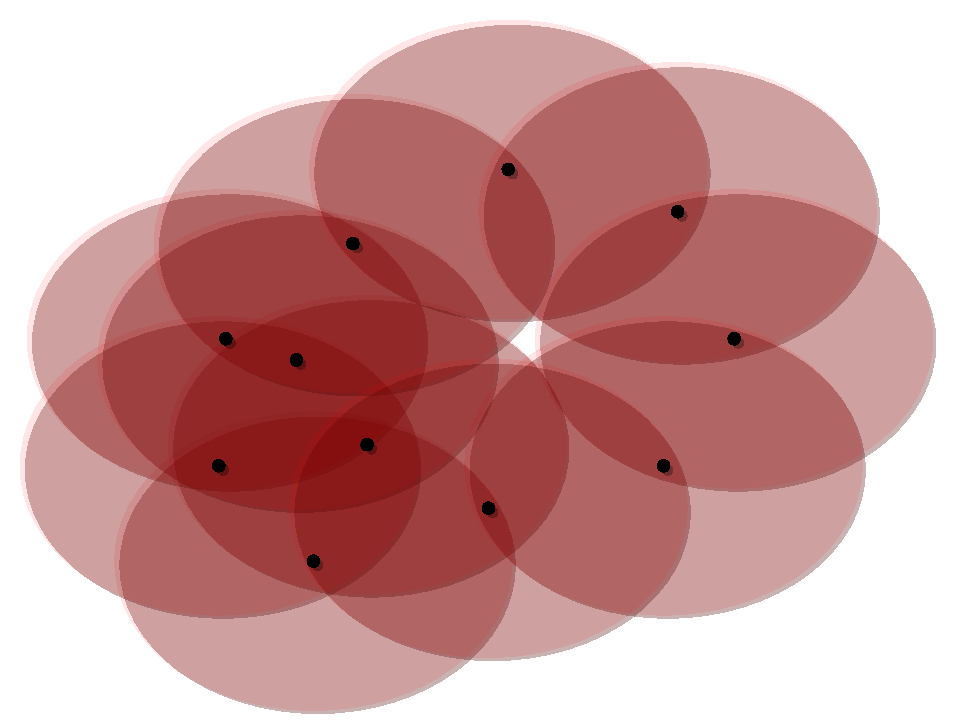
\includegraphics[scale=0.33]{figures/holes_cover.pdf}
    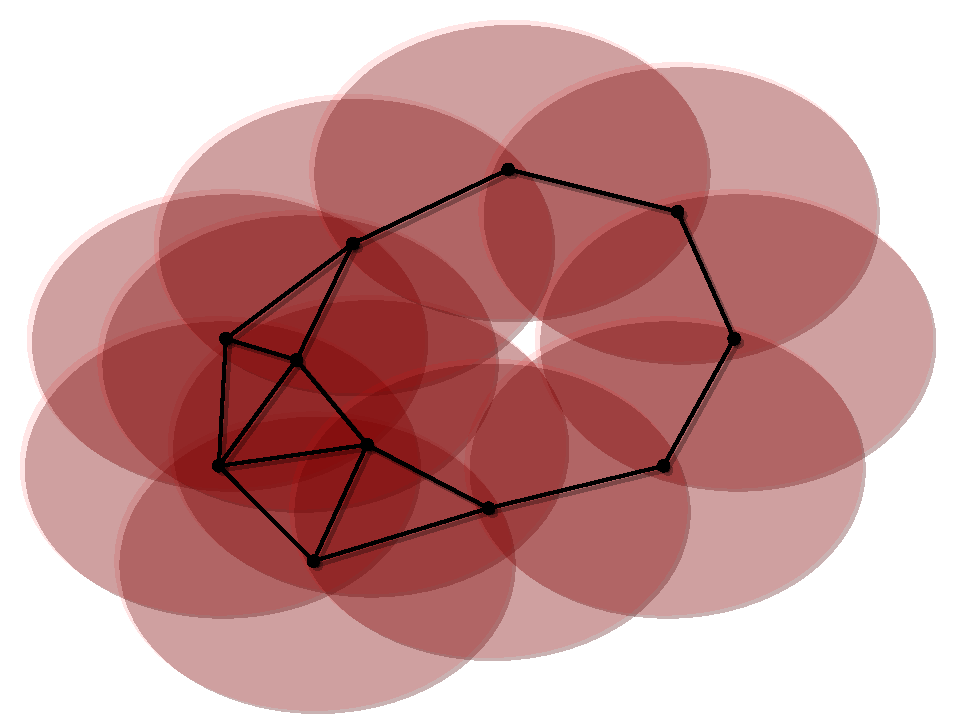
\includegraphics[scale=0.33]{figures/holes_edges.pdf}
    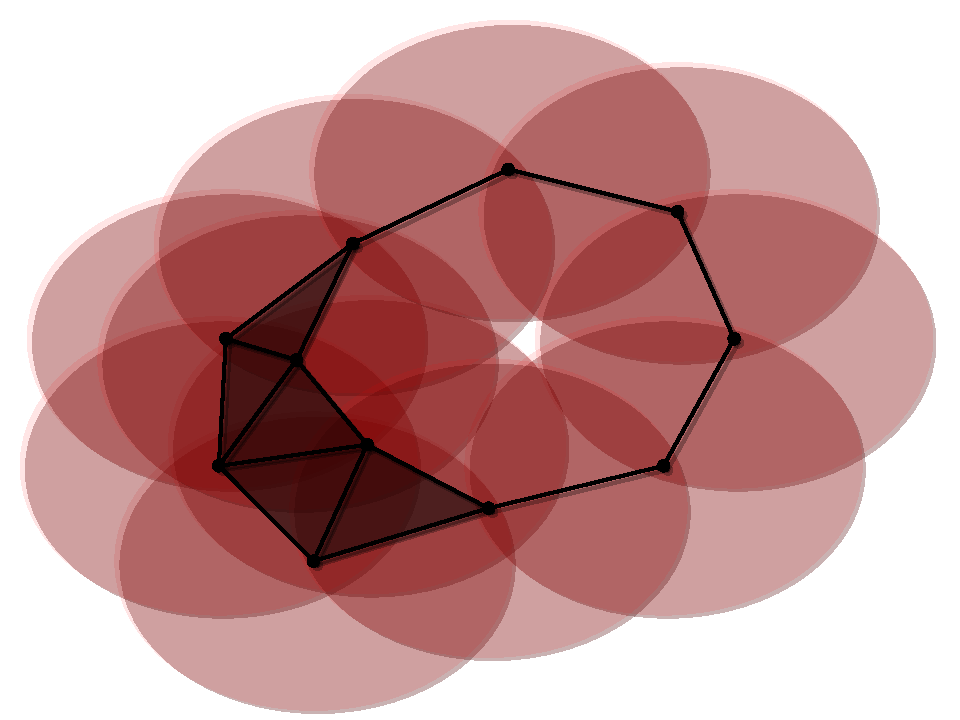
\includegraphics[scale=0.33]{figures/holes_complex.pdf}
     \caption{(Left) The coverage regions of a collection of points $P$ at some scale $\alpha$.
            (Middle) The neighborhood graph with edges for each pair of points within pairwise distance $\alpha$.
            (Right) If we attempt to fill cycles in the graph with triangles identify a cycle that cannot be filled which reflects a gap in coverage}
     \label{fig:holes}
\end{figure}}

It is natural to think of a $k$-dimensional simplicial complex as the generalization of an undirected graph consisting of vertices and edges, collections of at most 2 vertices, to collections of sets of at most $k-1$ vertices.
Just as we have defined a hole in our graph $G$ as a cycle that cannot be filled with triangles, we define a $k$-dimensinal hole in a simplicial complex as a $k$-cycle that cannot be filled with $(k+1)$-simplices.
In the next section we will formally define $k$-cycles and introduce simplicial homology as a tool for identifying when and which cycles cannot be filled.

\paragraph{Coordinate-free Communication}
In a coordinate-free sensor network each sensor, represented by a point in $P$, is capable of detecting nodes which are sufficiently ``close.''
That is, there is some radius of communication $\delta > 0$ such that two nodes $p, q\in P$ such that $\dist(p, q) \leq\delta$ are capable of communication.
Note that, although sensors can communicate within this distance they are not able to measure the distance itself.

With this limited capability we can construct an undirected graph $G=(V, E)$ with vertices $V=P$ and edges $E = \{\{p, q\}\subset P\mid \dist(p,q)\leq\delta\}$.
Let $K$ be a simplicial complex with 0-simplices $\{v\}$ for all $p\in P$, 1-simpices $\{u, v\}\subset P$ for each edge in $E$, and 2-simplices $\{u,v,w\}\subset P$ whenever $\{\{\{u,v\},\{v,w\},\{u,w\}\}\subset E$.
This particular simplicial complex is known as the Vietoris-Rips complex.
It is also an example of a clique complex, where the simplices are the complete subgraphs (or cliques) in a given graph.
\begin{definition}
    The \textbf{(Vietoris-)Rips complex} is defined for a set $P$ at scale $\e > 0$ as
    \[ \rips_\e(P) = \left\{\sigma \subseteq P\mid \forall p,q\in\sigma,\ \dist(p, q)\leq \e\right\}. \]
\end{definition}

\paragraph{Coverage}
% In order to determine coverage we must at least assert that the coverage domain spanned by the points in $P$ does not contain any holes.
% Assuming the coverage radius of our sensors is equal to their communication radius $\delta$ we may define a hole in coverage as a cycle that cannot be ``filled'' with triangles (see Fig.~\ref{fig:holes}).

\figblock{%
\begin{figure}[htbp]
\centering
    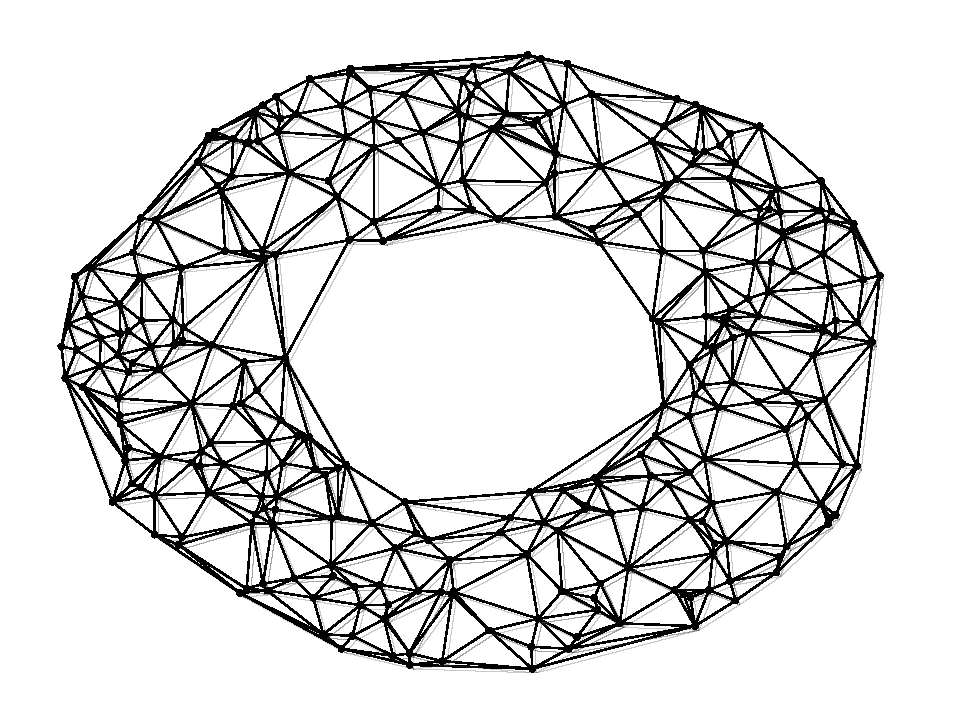
\includegraphics[scale=0.33]{figures/boundary_graph.pdf}
    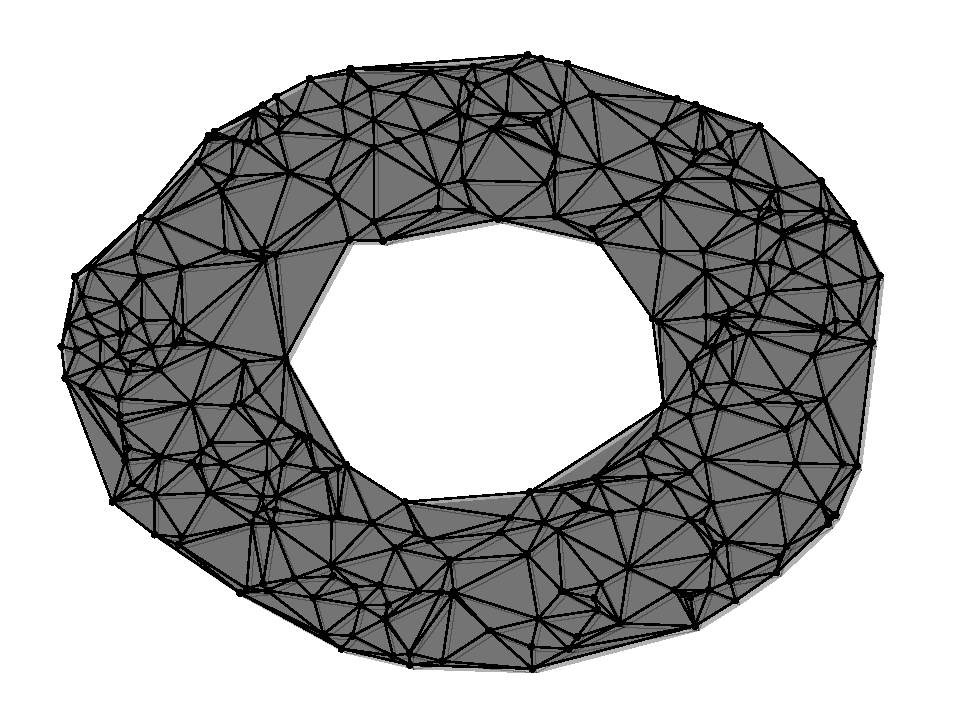
\includegraphics[scale=0.33]{figures/boundary_complex.pdf}
    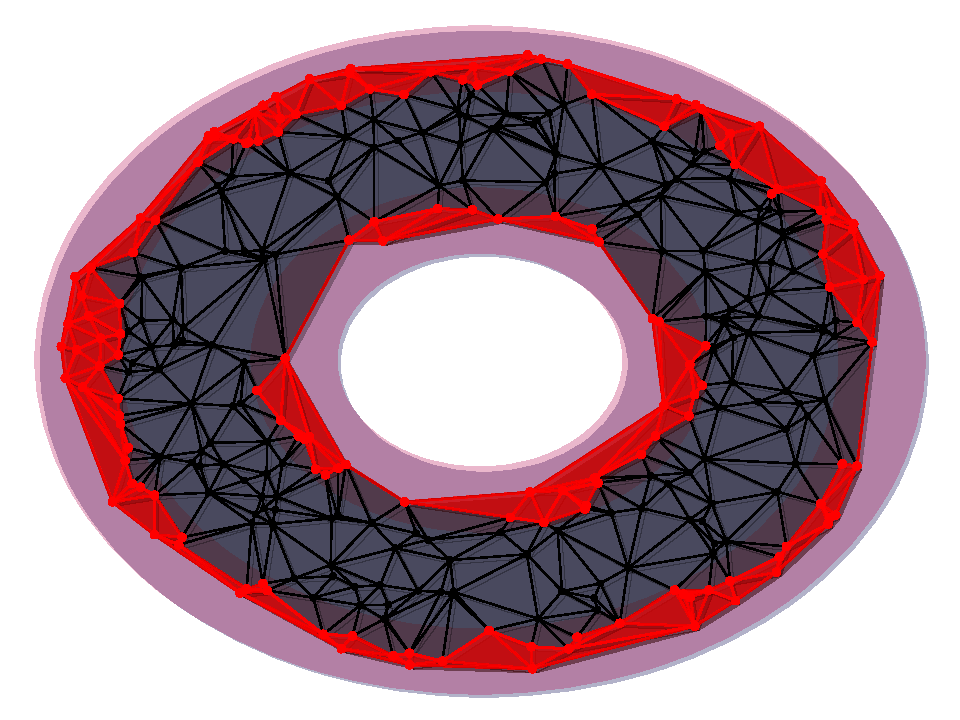
\includegraphics[scale=0.33]{figures/boundary_complex_domain_fence.pdf}
    % 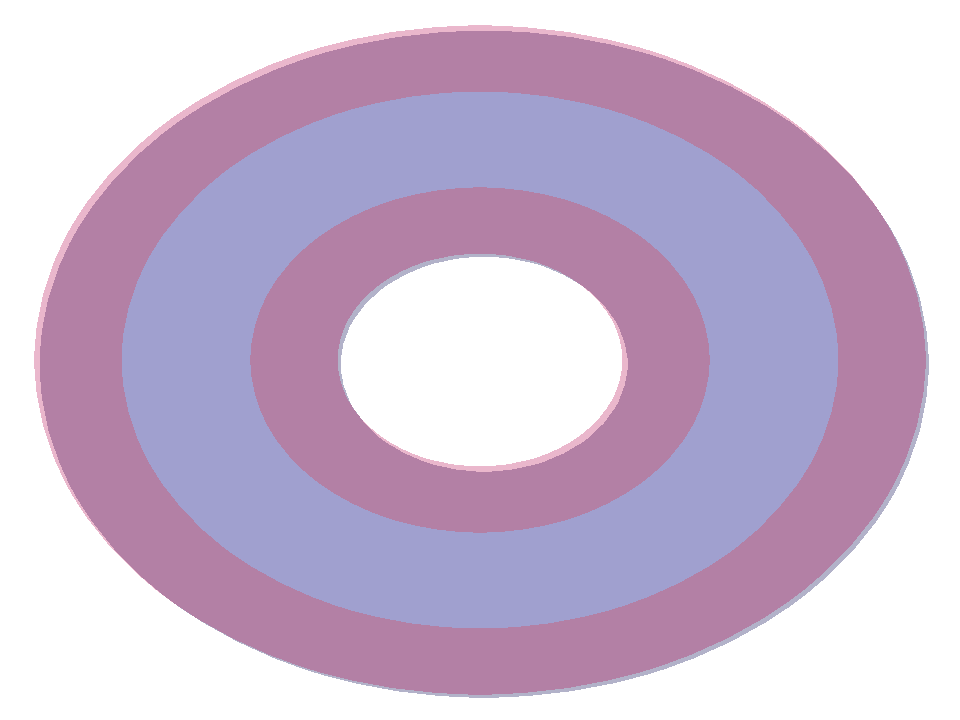
\includegraphics[scale=0.24]{figures/boundary_domain.pdf}
     \caption{(Left) The neighborhood graph of a sensor network with a large ``hole''.
            (Middle) A 2-dimensional simplicial complex with no gaps in coverage, but an unfilled cycle.
            (Right) By allowing nodes to identify the boundary (in red) we can confirm coverage of complex domains.}
     \label{fig:boundary1}
 \end{figure}}

If a sensor network $P$ covers a domain at scale $\e$ the topology of the domain is reflected in $\rips_\e(P)$.
However, as we will see, this does not necessarily give a tight bound on the minimum radius for coverage.
In fact, if the coverage region of of a sensor network at scale $\alpha$ has no gaps, then the minimum coverage radius required is a constant factor smaller than $\alpha$.
This point is made clear by an interleaving of the Rips with another simplicial complex known as the \v Cech complex.

\begin{definition}
    The \textbf{\v Cech complex} of a finite collection of points $P$ at scale $\e > 0$ is defined
    \[ \cech_\e(P) = \left\{\sigma \subseteq P\mid \bigcap_{p\in \sigma}\ball_\e(p)\neq \emptyset \right\}. \]
\end{definition}
The \v Cech complex is a special case of a more general construction known as the \textbf{nerve} $\N(\U)$ of a collection of sets $\U = \{U_i\}_{i\in I}$, where $I$ is any indexing set.
The nerve of $\U$ is defined as the simplicial complex with vertex set $I$ such that $\sigma\subseteq I$ is a simplex if and only if
\[
  \bigcap_{i\in \sigma} U_i\neq \emptyset.
\]
The collection $\U$ is a \textbf{good cover} if for each $\sigma\subset I$ the set $\bigcap_{i\in\sigma} U_i$ is contractible or empty.
The \textbf{Nerve Lemma} states that if $\U$ is a good cover then its nerve $\N(\U)$ is homotopy equivalent to $\bigcup_{i\in I} U_i$.
That is, for a set of nodes $P\subset\D$ such that $\U = \{\ball_\e(p)\mid p\in P\}$ is a good cover the nerve $\N(\U)$ is homotopy equivalent to $P^\e = \bigcup_{p\in P} \ball_\e(p)$.
It follows that the \v Cech complex $\cech_\e(P)$ of $P$ at scale $\e$ is a suitable representation of the coverage region $P^\e$.

\paragraph{Coordinate-free Coverage}
We will assume that the coverage radius of our sensor network is equal to the radius of communication.
In order to construct the \v Cech complex our sensors must be able to measure not only the proximity of neighboring nodes, but the precise distance between them.
Fortunately, the \v Cech and Rips complexes of a finite metric space are closely related by a result that follows from Jung's Theorem~\cite{jung01uber} relating the diameter of a point set $P$ and the radius of the minimum enclosing ball:
\[\cech_{\e/\jungd}(P)\subseteq\rips_\e(P)\subseteq\cech_\e(P)\subseteq\rips_{\jungd\e}(P),\]
where the constant $\jungd = \sqrt{\frac{2d}{d+1}}$ (see~\cite{buchet15efficient}).

Equipped with this interleaving we are now ready to define all conditions necessary for verifying coverage in a coordinate-free sensor network.
Specifically, we will introduce a second radius of communication $\gamma\geq 3\alpha$ that will allow us to lower $\gamma$, which will remain our coverage radius, so that homomorphism on (relative) homology induced by the inclusion of Rips complexes $\rips_\delta(P)\to\rips_\gamma(P)$ reflects that of the \v Cech complex, and therefore the coverage domain.

% In order to \textit{verify} coverage by we need our network to sufficiently sample the extent of our domain.
% Moreover, if there are gaps in coverage, we would like to know if they are due to insufficient sampling or to a gap in the domain itself.
% Let $\B\subset\D$ be the \textbf{boundary} of our domain and let our sensors detect when they are within the communication radius of $\B$.
% Let $Q = \{p\in P\mid \min_{x\in\B}\dist(x, p)\}$ be the set of \textbf{boundary nodes} in $P$.
% The set $Q$ induces a \textbf{subcomplex} $\rips_\alpha(Q)$ of $\rips_\alpha(K)$ restricted to nodes in $Q$.
% % Assuming there are no holes in our network no path from a point in $P\setminus Q$ to a point outside our domain  without crossing a simplex in $K\mid_Q$.
%
% % \textbf{TODO} Section overview.
% % We will show how this construction is used to verify coverage of a specific subset of a bounded domain $\D$ with a tight bound on the coverage radius.
%
% % Note that the communication radius is far from a tight bound on the coverage radius.

% Throughout we have been using the Rips complex as a discrete representation of our coverage domain by assuming the sensor coverage radius is equal to the communication radius.

% section complexes (end)

  % !TeX root = ../../main.tex

For a simplicial complex $K$ let $C_k(K)$ denote the vector space over a field $\F$ consisting of linear combinations of $k$-simplices in $K$ known as \textbf{$k$-chains}.
These vector spaces are connected by \textbf{boundary maps} $\partial_k:C_k(K)\to C_{k-1}(K)$ which are linear transformations taking basis elements of $C_k(K)$ to the abstract sum of basis $(k-1)$-simplex faces.
The collection of chains and boundary maps forms a sequence of vector spaces known as the \textbf{chain complex} of $K$.

An important property of the boundary maps $\partial_k$ is that the composition of subsequent boundary maps is zero.
That is, $\partial_k\circ\partial_{k-1} = 0$ for all $k$.
As a result the image of $\partial_{k+1}$, denoted $\im~\partial_{k+1} = \{\partial_{k+1}c\mid c\in C_{k+1}(K)$ is a subspace of the kernel, $\ker~\partial_k = \{c\in C_k(K)\mid \partial_k c = 0\}$, of $\partial_k$.
A \textbf{$k$-cycle} of $\C$ is a $k$-chain with empty boundary---an element of $\ker~\partial_k$.
Two cycles in $\ker~\partial_k$ are said to be \textbf{homologous} if they differ by an element of $\im~\partial_{k+1}$.
The \textbf{$k$th homology groups} of $K$ is the quotient group $\hom_k(K) = \ker~\partial_k/\im~\partial_{k+1}$.
Elements of $\hom_k(K)$ are equivalence classes $[x]$ of homologous $k$ cycles.
That is, if $[x] = [y]$ for any $x,y\in C_k(K)$ then $x = y +\partial_{k+1}z$ for some $z\in C_{k+1}(K)$.


% The rank of a homology group is of particular importance and is known as the \textbf{Betti number} $\beta_k = \rank~ \hom_k(K)$.
% These topological invariants can be thought of as counting the number of $k$-dimensional ``holes'' in a topological space, where $0$-dimensional holes are connected components, $1$-dimensional holes are loops, $2$-dimensional holes are voids, and so on.
% Note that this is the same notion which motivated our use of simplicial complexes for determining coverage---a $1$-dimensional hole exists if a gap in a neighborhood graph cannot be filled by triangles.

While we have chosen to define simplicial homology for ease of exposition we will primarily be using singular homology over a field $\F$ so that the homology groups $\hom_k(X)$ of a topological space $X$ are vector spaces.
For a full treatment of both singular and simplicial homology see Hatcher~\cite{hatcher01}.

\paragraph{Relative Homology}

Let $(X, Y)$ be a pair of topological spaces (or pair of simplicial complexes).
The relative chain groups $C_k(X, Y) = C_k(X) / C_k(Y)$ consist of equivalence classes of chains in $C_k(X)$ that differ by chains in $C_k(Y)$.
We note that the boundary map $\partial_k$ on $C_k(X)$ induces a boundary map on the quotient $C_k(X, Y)$ such that $\partial_k(y) = 0$ for all $y\in C_k(Y)$.

The \textbf{$k$th relative homology group} $\hom_k(X, Y)$ consists of homology classes of relative cycles---chains in $C_k(X)$ whose boundaries vanish or lie in $Y$.
That is, a relative $k$-cycle can either be a cycle in $C_k(X)$ or a chain in $C_k(X)$ with a boundary in $C_{k-1}(Y)$.
We will make extensive use the \textbf{excision} axiom of homology which states that for any $A\subset Y$ such that $\cl_X(A)\subseteq \intr_X(Y)$ the inclusion of pairs $(X\setminus A, Y\setminus A)\hookrightarrow (X, Y)$ induces isomorphisms on relative homology groups $\hom_k(X\setminus A, Y\setminus A)\cong\hom_k(X, Y)$.

\paragraph{Exact Sequences}

A sequence $A\xrightarrow{i} B\xrightarrow{j} C$ is said to be \textbf{exact} if $\im~i = \ker~j$.
An exact sequence $0\to A\to B\to C\to 0$ is said to be \textbf{short exact}.
In general, any exact sequence $\ldots\to A\to B\to C\to\ldots$ is referred to as a long exact sequence.

For any pair of topological spaces $(X, Y)$ the \textbf{long exact sequence of the pair} is the exact sequence
\[ \ldots\to\hom_{k+1}(X, Y)\xrightarrow{\partial_{k+1}} \hom_k(Y)\xrightarrow{i_k} \hom_k(X)\xrightarrow{j_k}\hom_k(X, Y)\xrightarrow{\partial_k}\hom_{k-1}(Y)\to\ldots.\]
Here the map $\partial_k$ is the connecting homomorphism which is induced by the boundary map on $C_k(X, Y)$.

% section homology (end)

  % !TeX root = main.tex

\subsection{Persistent Homology}

\paragraph*{\textbf{Functions and Filtrations}}

\figblock{%
\begin{figure}[htbp]
\centering
    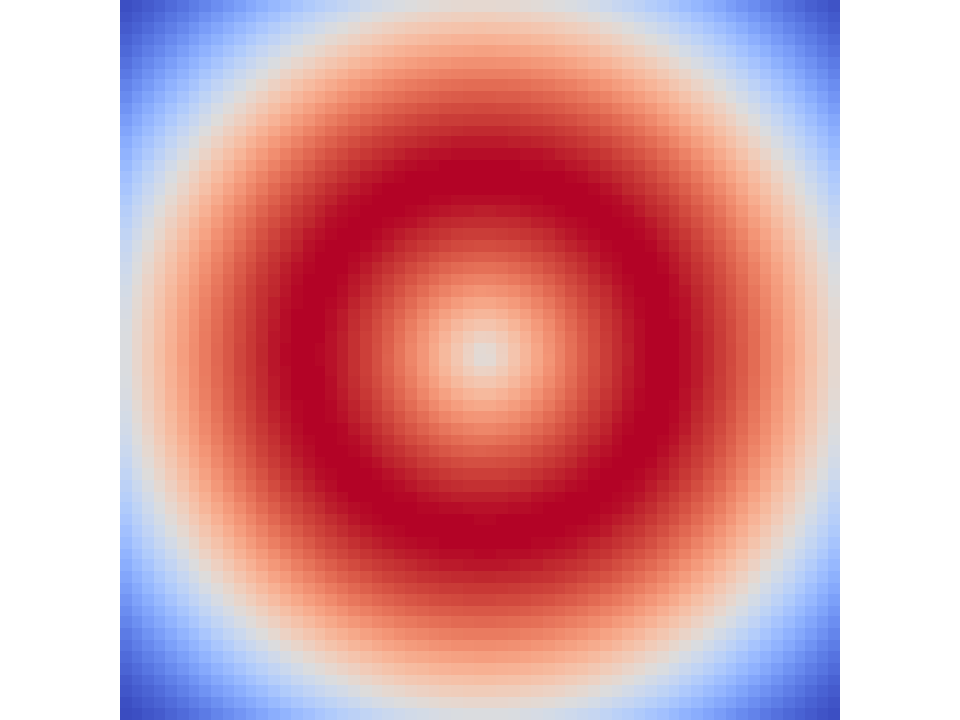
\includegraphics[scale=0.45]{figures/fgrid.pdf}
    % 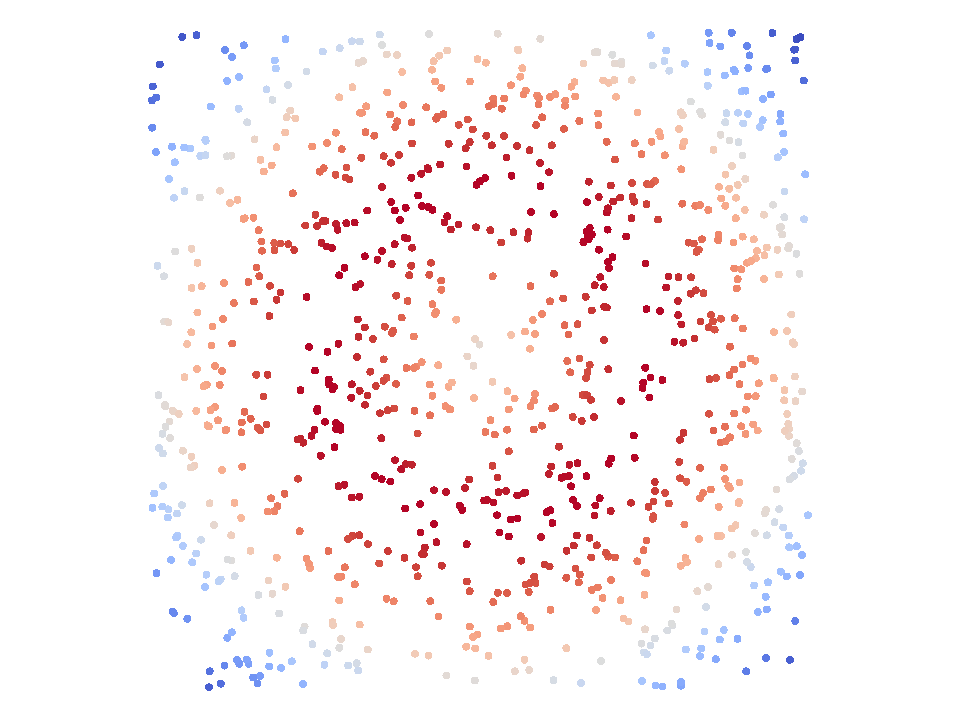
\includegraphics[scale=0.45]{figures/fsample.pdf}
    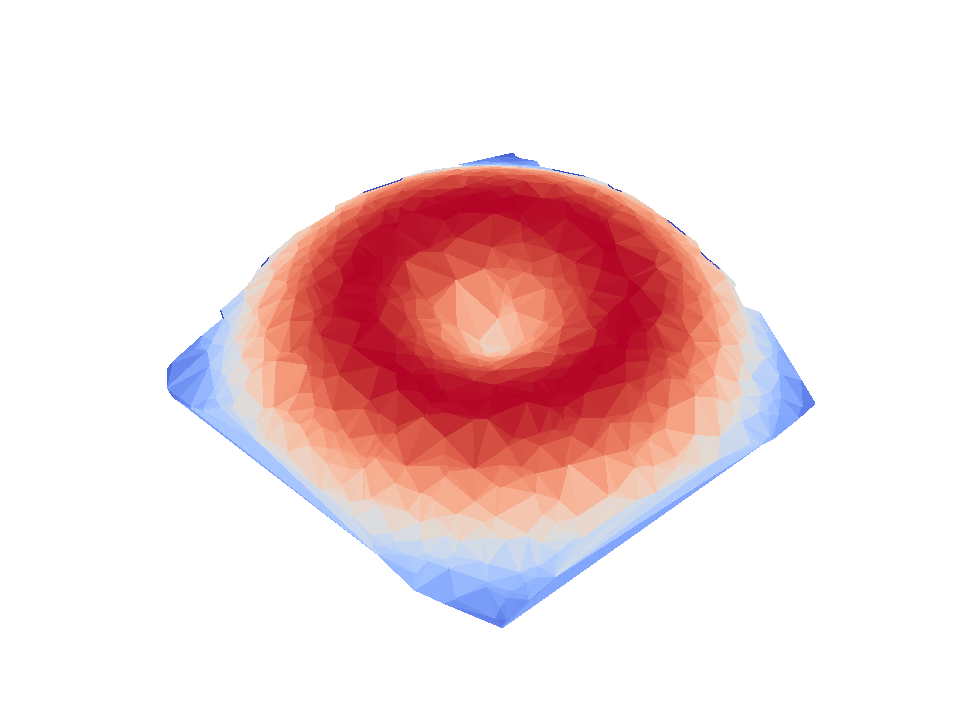
\includegraphics[scale=0.55]{figures/fcomplex.pdf}
    \caption{(Left) Continuous function on the plane.
            % (Middle) Function values on random sample.
            (Right) Function values on a random sample extended to a continuous piecewise linear approximation on a 2-dimension simplicial as the $z$-axis.}
    \label{fig:function}
\end{figure}}

Suppose we have some real valued function $f:\D\to\R$ and endow our sensors with the ability to measure this function at their points $P$.
If we know our network covers the domain we may construct a simplicial complex which captures its topology in a discrete structure.
We may therefore integrate the sparse measurements provided by the sensors throughout the simplicial complex to capture the topology of the function itself.
Not only do we now have a discrete approximation of the function but an ordering on the simplices of the complex which may be used to explore the evolution of the topological structure of the function.

This leads to a more general notion defined for a sequence of topological spaces, which we may take as sublevel sets of the function on the domain.
\begin{definition}
    Let $f:\D\to\R$ be a function on a topological domain $\D$ and let $I_0, I_1,\ldots$ be a sequence of intervals $I_i = [a_i, b_i)$ that covers the image of $f$ on $\D$.
    Let and $X_i = \{x\in\D\mid a_i\leq f(x) < b_i\}$ be topological subspaces connected by inclusion maps $X_i\to X_{i+1}$.
    A \textbf{filtration} is the resulting sequence of topological spaces
    \[X_0\to X_1\to\ldots X_i\to X_{i+1}\to\ldots .\]
\end{definition}
A filtration $\{K_i\}_{i=1,\ldots,n}$ may also be interpreted as a sequence of simplicial maps, each an inclusion $K_i\to K_{i+1}$.
This induces an algebraic sequence of homomorphisms on homology by functoriality, for all $k$:
\[ H_k(X_0)\to H_k(X_1)\to\ldots\to H_k(X_i)\to H_k(X_{i+1})\to\ldots . \]
This sequence encodes the local topological changes that occur at each step of the filtration.
Global information is encoded in terms of the \textbf{birth} and \textbf{death} of homology classes, represented as a \textbf{persistence diagram} or \textbf{barcode}.

% \vspace{0.25in}
% \textbf{TODO} Persistence diagram of a function on a simplicial complex
% \vspace{0.25in}

% \figblock{%
% \begin{figure}[htbp]
% \centering
%     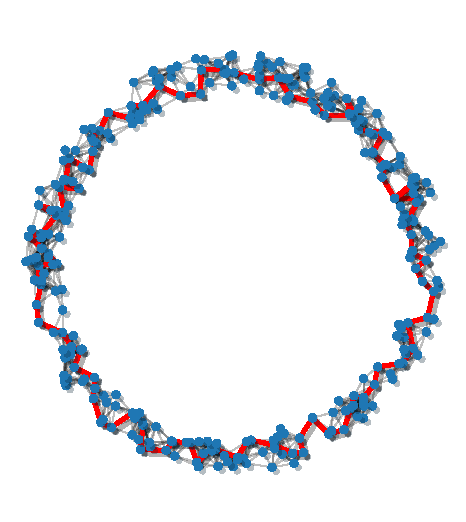
\includegraphics[scale=0.9]{figures/homology_cycle.pdf}\hspace{10ex}
%     % 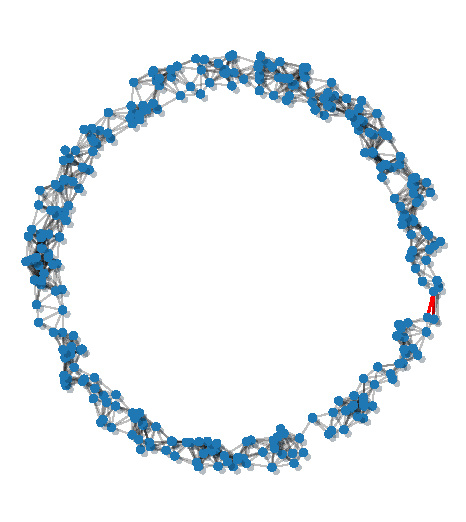
\includegraphics[scale=0.6]{figures/cohomology_cocycle.pdf}
%     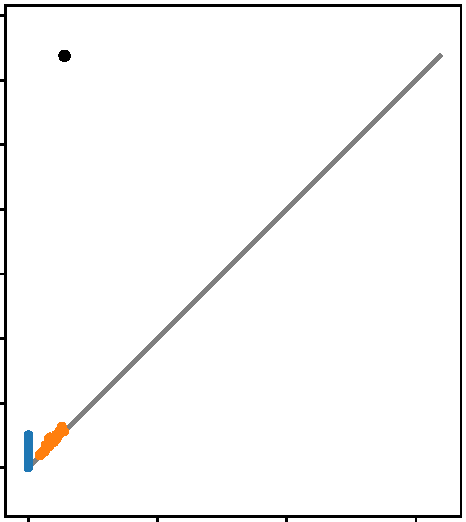
\includegraphics[scale=0.8]{figures/homology_dgm.pdf}
%     \caption{The representative cycle of a significant feature in the persistent homology of rips filtration of a noisy circle.
%             The birth of the feature indicated on the persistence diagram (right) corresponds to the scale of the rips complex shown (left) when the circle, a 1-cycle, is born.
%             The death of this feature corresponds to the scale of the rips complex at a larger scale (not shown) when a triangle first fills the interior of the circle.
%             This scale is approximately the length of the edges in the smallest equilateral triangle with sample points as vertices that contains the centroid of the sample.
%             This illustrates the geometric information encoded in the persistence diagram of geometric complexes as it is within a constant factor of the radius of the circle.}
%     \label{fig:cycle_diagrams}
% \end{figure}}
%
% Given a simplicial complex $K$ on a set of points $P\subset\D$ and a function $f:\D\to\R$ we may construct a filtration $\{K_i\}_{i=1,2,\ldots}$ by ordering the simplices by their function values.
% For example, $f(\sigma) = \max_{v\in\sigma} f(v)$ for any simplex $\sigma\in K$.
% The resulting filtration is now a sequence of simplicial maps, each an inclusion $K_i\to K_{i+1}$, which induces a sequence of homology groups.

% \subsection{Persistent Homology}
%
% \begin{figure}[htbp]
% \centering
%     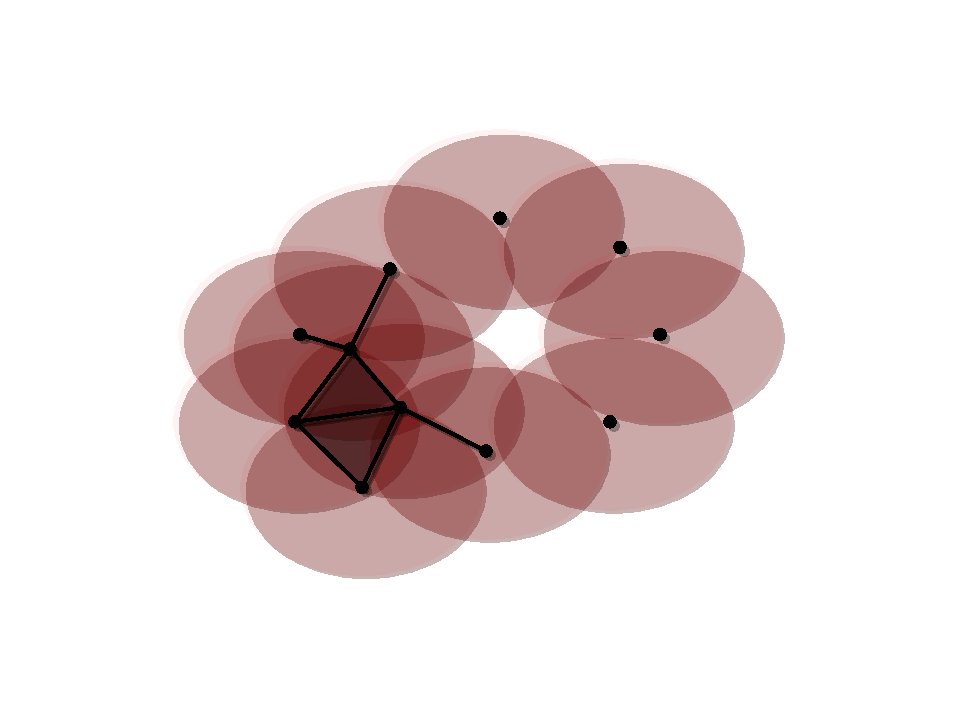
\includegraphics[scale=0.4]{figures/persist06.pdf}
%     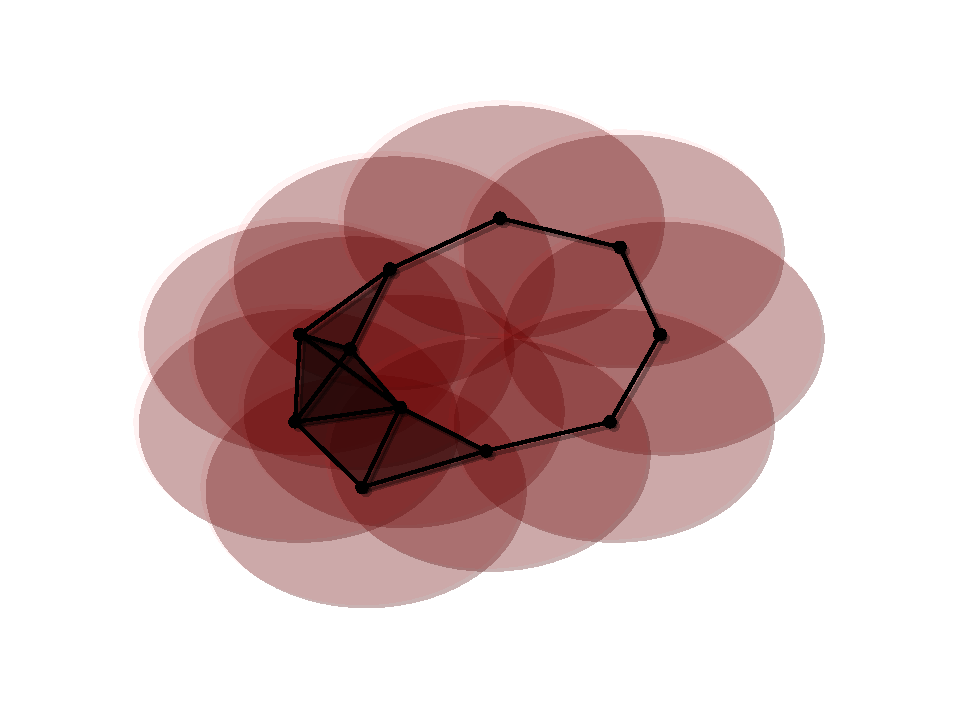
\includegraphics[scale=0.4]{figures/persist08.pdf}
%     % 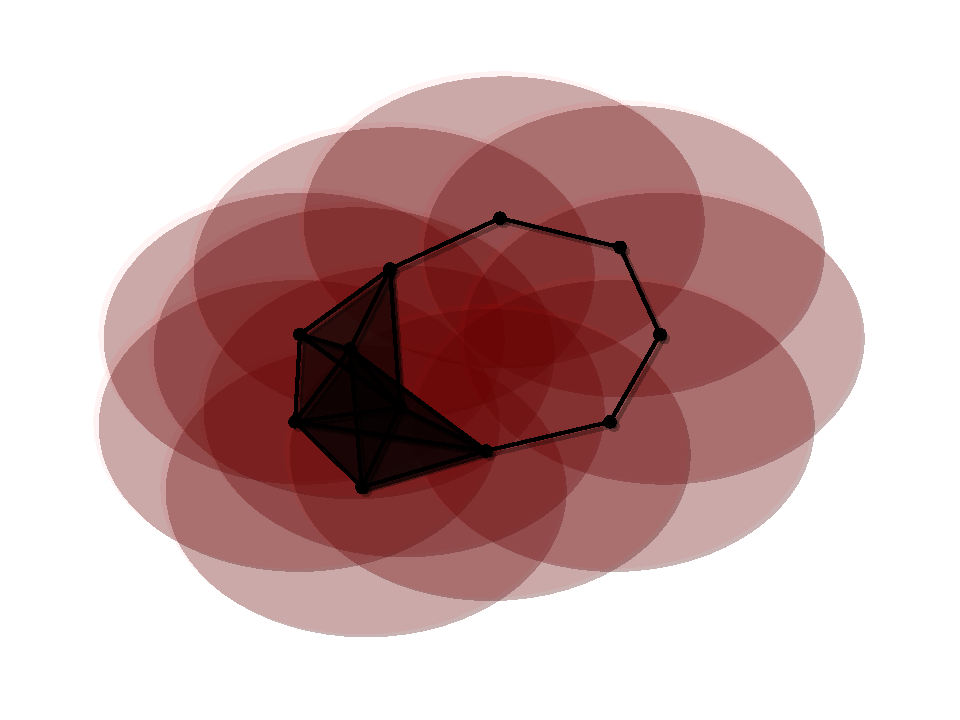
\includegraphics[scale=0.4]{figures/persist10.pdf}
%     % 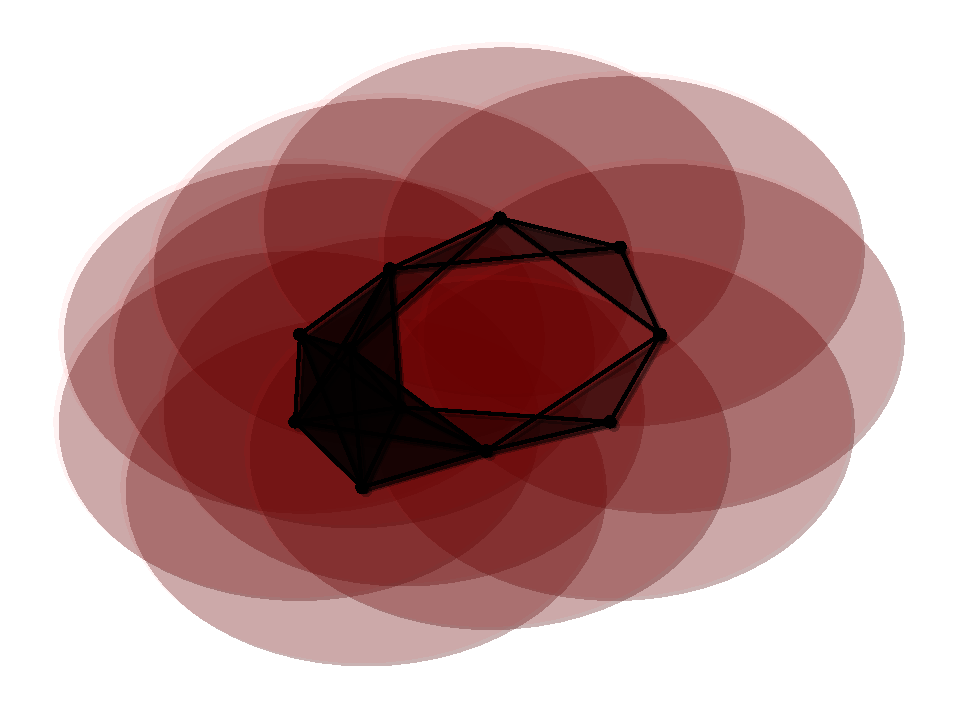
\includegraphics[scale=0.4]{figures/persist12.pdf}
%     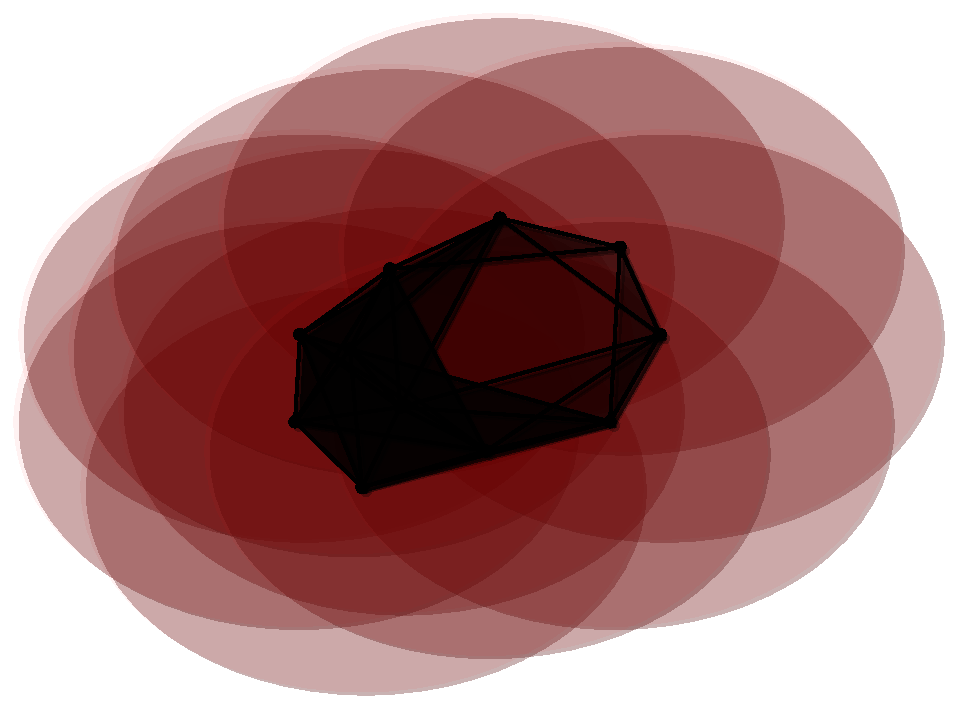
\includegraphics[scale=0.4]{figures/persist14.pdf}
%     \caption{A filtration of rips complexes at scales 0.6, 0.8, and 1.4 illustrating a point $(0.8, 1.4)$ in the corresponding persistence diagram. The 1-cycle that is born at scale 0.8 persists until it dies at scale 1.4.}
%     \label{fig:persist}
% \end{figure}
%
% % \vspace{0.25in}
% % \textbf{TODO} ``Metric'' persistence.
% % \vspace{0.25in}
%
% % Topological data analysis is an emerging field in the intersection of data analysis and algebraic topology which extends the notion of homology and cohomology groups to a more analytical tool known as \textbf{topological persistence}.
% % Where simplicial homology identifies invariants of a static simplicial complex persistent homology tracks the evolution of a sequence of nested simplicial complexes which provide a more detailed topological signature, in addition to relevant geometric information.
%
% Just as we can construct a filtration from a function on a simplicial complex we can construct a filtration from the metric induced on our sample by the domain.
% Let $P$ be a finite metric space with $m$ points and let $K = \rips_\alpha(P)$ be the Rips complex of $P$ at scale $\alpha$ consisting of $n$ simplices.
% We can order the simplices $\sigma_1,\ldots,\sigma_n$ by the minimum pairwise distance between their vertices by first applying an arbitrary ordering on the vertices $v_1,\ldots,v_m$ and letting $\sigma_i = \{v_i\}$ for $i=1,\ldots,m$ so that $K_i = \{\sigma_1,\ldots, \sigma_m\}$.
% We can then build a filtration $\K = \{K_i\}_{i=1,\ldots,n}$ so that $K_i = \rips_\e(P)$ where $\e = \max_{u,v\in\sigma_i}\dist(u,v)$ by adding one simplex at a time, breaking ties first by dimension, then by the ordering on their constituent vertices.
% A $k$-dimensional feature is identified when a $(k+1)$-simplex $\sigma$ is added that kills a $k$-cycle $\gamma$.
% In the persistence diagram, this feature would be represented by a point $(b, d)$ where $b$ is the smallest scale for which the $k$-cycle appears
% \[ \tau\in\rips_b(P)\text{ for all }\tau\in\gamma\]
% and $d = \max_{u,v\in\sigma}\dist(u,v)$ is the scale at which $\sigma$ enters the filtration.
% The result is a collection of points $(b_i, d_i)$ in the plane for each dimension $k$ known as the persistence diagram, denoted $\dgm_k(\K)$.
% A persistence diagram is depicted on the right in Fig.~\ref{fig:cycle_diagrams}.

\paragraph*{\textbf{Persistent Homology.}} % (fold)
\label{par:persistent_homology}

Given a filtration $\mathcal{F} = \{F_\alpha\}_{\alpha\in\R}$ the inclusions $F_\alpha\hookrightarrow F_\beta$ induce homeomorphisms between homology groups $h_*^{\alpha,\beta} : H_*(F_\alpha)\to H_*(F_\beta)$.
The \emph{persistent homology modules} of $\F$ are the pairs
\[\mathcal{H}_*(\F) = (\{H_*(F_\alpha)\}_{\alpha\in\R}, \{h_*^{\alpha,\beta}\}_{\alpha\leq\beta\in\R}).\]

The persistent homology modules of a filtration $\F$ are each given by a signature known as a \emph{persistence diagram}, denoted $\Pers_*(\F)$, where $\Pers(\F)$ is used to refer to the collection of persistence diagrams of all dimensions.
Unless otherwise noted we will refer $\Pers(\F)$ as the persistence diagram of $\F$.

The space of persistence diagrams is a metric space $(\PPers, \dist_B)$ under the \emph{bottleneck distance} which is defined for diagrams $A, B$, taken as multisets in $\R^2$ equipped with the $l^\infty$-norm, as
\[\dist_B(A, B) = \min_{\gamma:A\to B}\max_{p\in A} \| p- \gamma(p)\|_\infty\]
where $\gamma$ ranges over all bijections from $A$ to $B$.

\paragraph*{\textbf{Stability of Persistent Homology.}} % (fold)
\label{par:stability_of_persistent}

The persistent homology of Rips filtrations constructed from point clouds in euclidean space is closely related to the sequence of metric balls growing around the point cloud as the persistent homology of both gives a signature for distance to the point cloud.
In particular, the persistent homology of the Rips complex of a point cloud approximates that of the distance to the point cloud as a function on the underlying metric space.

\figblock{%
\begin{figure}[htbp]
\centering
    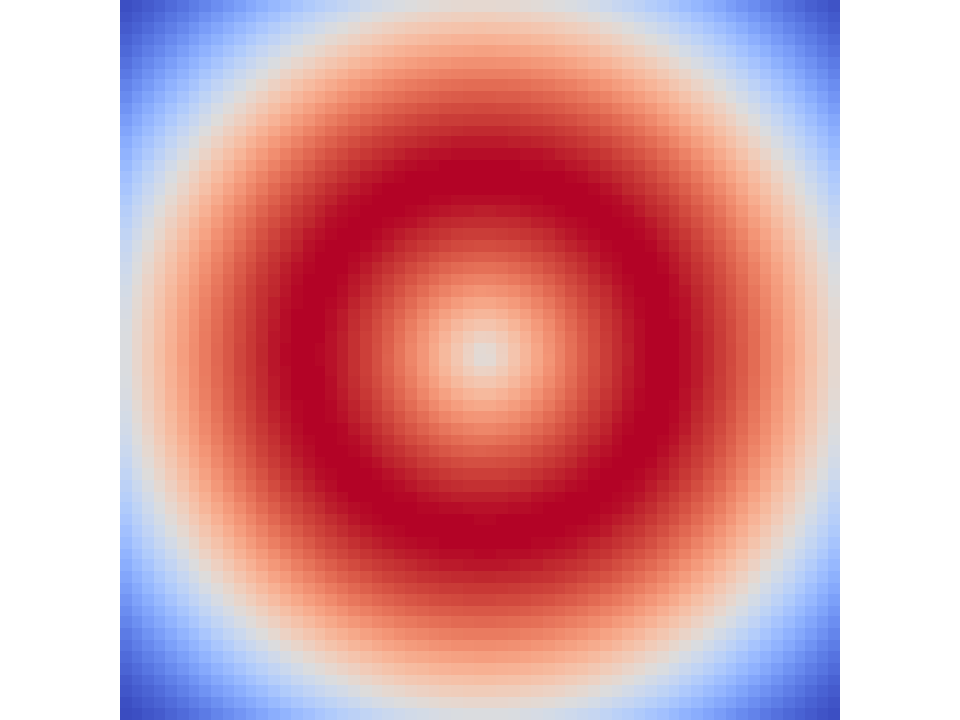
\includegraphics[width=0.29\textwidth,trim={0 -1.5cm 0 0},clip]{figures/fgrid.pdf}
    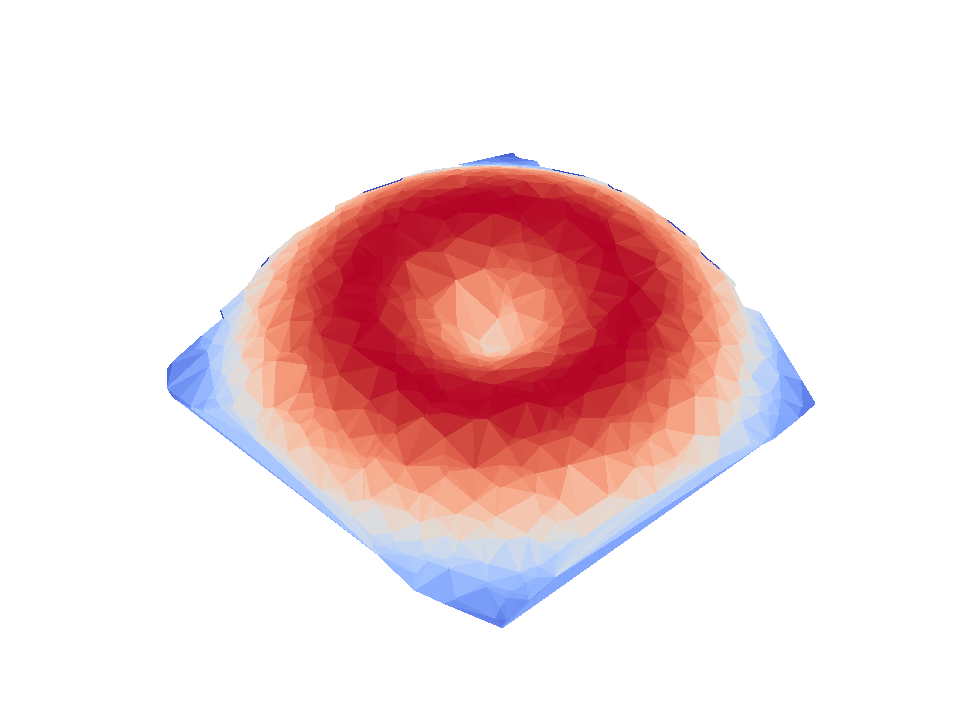
\includegraphics[width=0.4\textwidth]{figures/fcomplex.pdf}
    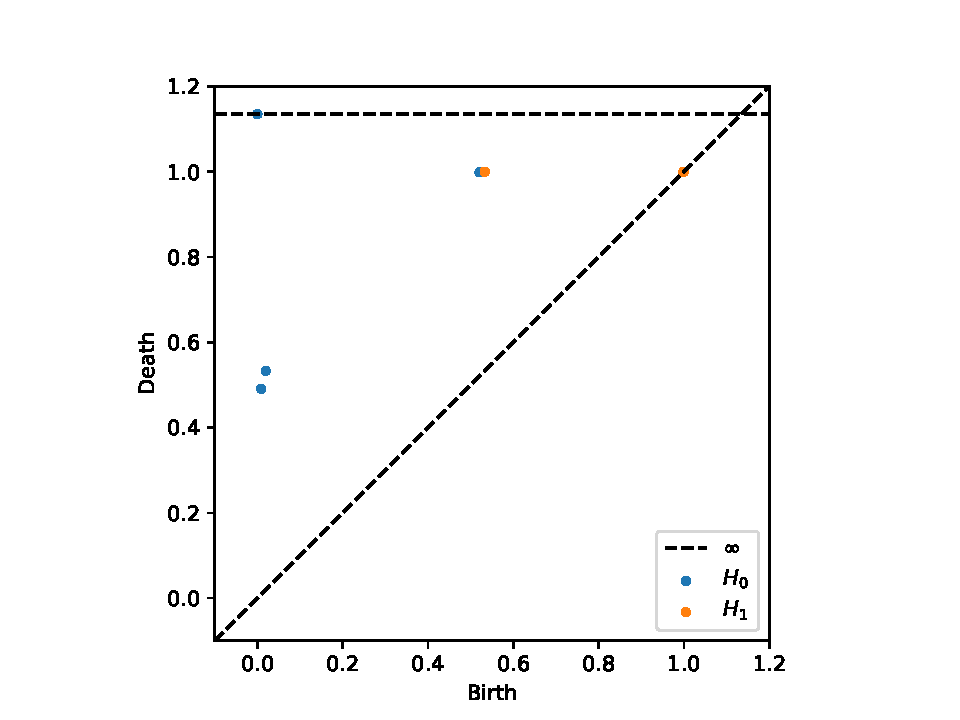
\includegraphics[width=0.29\textwidth,trim={2cm 0cm 2cm 1cm},clip]{figures/fdgm.pdf}
    \caption{(Left) Continuous function on the plane.
            (Middle) Function values (as $z$-axis) on a random sample extended to a simplicial complex.
            (Right) Persistence diagram of an induced filtration.}
    \label{fig:function}
\end{figure}
}

More generally, the persistent homology of a real-valued function captures the changes in the homology groups of its \emph{sublevel-sets}---the set of points with function values below a given scale.
The distance to a point cloud is a real-valued function with sublevel-sets equal to the union of metric balls at a given scale.
Under certain conditions we can approximate the persistent homology of a real-valued function given only its values on a finite subset of its domain.

Given a topological space $X$ and a real-valued function $f:X\to\R$ the \emph{sublevel-set filtration} of $f$ is the sequence $\{X^f_\alpha\}_{\alpha\in\R}$ of sublevel-sets $X^f_\alpha = f^{-1}(-\infty, \alpha]$.
We define a metric $\dmax$ between two real-valued functions $f,g:X\to\R$ by taking the maximum difference of the functions on any point, i.e.
\[ \dmax(f, g) := \max_{x\in X} |f(x) - g(x)|. \]

\begin{lemma}\label{lem:interleave}
    Let $X$ be a topological space and $f,g: X\to\R$ are tame functions such that $\dmax(f, g)\leq\e$.
    Then the sublevel-set filtrations $\{X_\alpha^f\}_{\alpha\in\R}$ of $f$ and $\{X_\alpha^g\}_{\alpha\in\R}$ of $g$ are $\e$-interleaved.
\end{lemma}

The following is a standard result in the stability of persistence diagrams.

\begin{lemma}\label{lem:stability}
    If two filtrations $\F$ and $\F'$ are $\e$-interleaved then
    \[ \dist_B(\Pers(\F), \Pers(\F'))\leq\e. \]
\end{lemma}

The persistent homology modules of the sublevel-set filtration $\{X^f_\alpha\}_{\alpha\in\R}$ are referred to as the persistent homology modules $\mathcal{H}_*(f)$ of $f$ with its diagram denoted $\Pers(f)$.

\begin{corollary}\label{cor:stability}
    If $X$ is a topological space and $f,g:X\to\R$ are tame functions then
    \[ \dist_B(\Pers(f), \Pers(g))\leq\dmax(f, g). \]
\end{corollary}

  % % !TeX root = main.tex

% \section{Background}
% \label{sec:background}

% \paragraph*{\textbf{Simplicial Complexes.}}
%
% A \textbf{simplicial complex} $K$ with vertex set $V$ is a collection of \textbf{simplices} $\sigma\subset V$ that is closed under taking subsets.
% We define a \textbf{pair of complexes} to be a pair $(K, L)$ where $K$ is a simplicial complex and $L$ is a subcomplex of $K$.
%
% Given a metric space $(X, d)$ we define the $\e$-offsets of a point $p\in X$ as \[\ball(p, \e) = \{x\in X\mid d(x, p)\leq \e\}.\]
% For a subset $P\subseteq X$ the \emph{nerve} of a family $\{\ball(p,\e)\}_{p\in P}$ is the abstract simplicial complex with vertex set $P$ with simplices corresponding to subsets of elements with nonempty intersections, and is known as the \emph{\v{C}ech complex}
% \[
%   \cech_\e(P) := \left\{\sigma \subseteq P\mid \bigcap_{p\in \sigma}\ball(p,\e)\neq \emptyset \right\}.
% \]
% The \textbf{(Vietoris-)Rips complex} of $P$ at scale $\e$ is defined as
% \[
%   \rips_\e(P) := \left\{\sigma \subseteq P \mid \{p,q\}\in\cech_\e(P) \text{ for all $p,q\in \sigma$}\right\}.
% \]
%
% For any metric space $(X, d)$ the \v{C}ech and Rips complexes of a subset $P\subset X$ are related by the following interleaving for all $\e > 0$
% \[ \cech_{\e/2}(P)\subseteq \rips_\e(P)\subseteq \cech_\e(P). \]
%
% \paragraph*{\textbf{Homology and Persistent Homology.}} % (fold)
% \label{par:homology_and_persistent_homology}
%
% Homology is a tool from algebraic topology that provides a topological signature for a shape that may be readily computed from a matrix representation of a finite simplicial complex through matrix reduction.
% The resulting signature is invariant under homeomorphisms and homotopy equivalences, and may be thought of as quantifying the components, loops, and voids in a topological space.
%
% Throughout, we assume singular homology over a field, where the \emph{$k$th homology group} of a space $X$ is a vector space denoted $H_k(X)$.
% We will write $H_*(X)$ to denote the homology of all dimensions.
% For a pair of spaces $(X,Y)$ with $Y\subseteq X$ the \emph{relative homology groups} gives the homology of $X$ relative to $Y$, and are denoted $H_*(X,Y)$.
%
% A \emph{filtration} is a sequence of topological spaces $\mathcal{F} = \{F_\alpha\}_{\alpha\in\R}$ that are nested by inclusions $F_\alpha\hookrightarrow F_\beta$ for $\alpha\leq\beta$.
% Each inclusion $F_\alpha\hookrightarrow F_\beta$ induces homeomorphisms between homology groups $h_*^{\alpha,\beta} : H_*(F_\alpha)\to H_*(F_\beta)$.

\paragraph*{\textbf{Analysis of Scalar Fields.}} % (fold)
\label{par:stability_of_persistent}

Figure~\ref{fig:function} depicts a function on a subset of the plane and its function values on the simplices of a simplicial complex defined on a subset of the plane.
The filtration given by ordering the simplices of this complex by their function values is known as an \emph{induced filtration}.
Chazal et. al. detail how to construct a filtration (in fact, the inclusion of two filtrations) that approximates the persistence diagram of the function itself~\cite{chazal09analysis} that has a natural application to measurements by coordinate-free sensor networks.
Extending our testbed to explore this result was a natural next step as it assumes coverage and the structures required are a subset of those used in the computation of the TCC.
This extension has led to promising results on applications to functions on coordinate-free networks over time as well as interesting theoretical questions on the role of the boundary in these experiments.

For a compact Riemannian manifold $X$, possibly with boundary, a point $x\in X$ and a real value $r\geq 0$, let $B_X(x, r) = \{y\in X\mid d_X(x,y) < r\}$ denote the open geodesic ball of center $x$ and radius $r$.
For all sufficiently small values $r\geq 0$ the ball $B_X(x,r)$ is said to be \emph{strongly convex} if for every pair of points $y,y'$ in the closure of $B_X(x, r)$, there exists a unique shortest path in $X$ between $y$ and $y'$, and the interior of this path is included in $B_X(x, r)$.
Let $\varrho(x) > 0$ be supremum of the radii such that this property holds.
The \emph{strong convexity radius} of $X$ is defined $\varrho(X) = \inf_{x\in X}\varrho(x)$.
Because $X$ is compact $\varrho(X)$ is known to be positive.
This quantity is required in order to apply the Nerve theorem in Theorem~\ref{thm:scalar}.
% In the following let $R_\delta^{\delta'}(P) = \im (R_{\delta}(P)\hookrightarrow R_{\delta'}(P))$ denote the image of the inclusion of Rips complexes of some set $P\subseteq X$ at scales $\delta\leq\delta'$.

\begin{theorem}[Theorem 2 of~\cite{chazal09analysis}]\label{thm:scalar}
    Let $X$ be a compact Riemannian manifold, possibly with boundary, and let $f:X\to\R$ be a $c$-Lipschitz function.
    Let also $P$ be a geodesic $\e$-sample of $X$.
    If $\e < \frac{1}{4}\varrho(X)$, then for any $\delta\in [2\e,\frac{1}{2}\varrho(X))$ and for any $k\in\N$, the $k$th persistent homology modules of $f$ and of the nested pair of filtrations $\{\rips_\delta(P_\alpha^f)\hookrightarrow \rips_{2\delta}(P_\alpha^f)\}_{\alpha\in\R}$ are $2c\delta$-interleaved.
    % $\{R_\delta^{2\delta}(P_\alpha^f)\}_{\alpha\in\R}$ are $2c\delta$-interleaved.
    Therefore, the bottleneck distance between their persistence diagrams is at most $2c\delta$.
\end{theorem}

\paragraph*{\textbf{Stability of Relative Persistent Homology.}} % (fold)
\label{par:stability_of_relative_persistent}

Let $(X, Y)$ be a pair of spaces with $Y\subseteq X$.
For $f:X\to\R$ we define a function $\tilde{f}$ on the pair $(X, Y)$ as the pair $(f, f\restriction_Y)$ where $f\restriction_Y:Y\to\R$ is the restriction of $f$ to $Y$.
The \emph{sublevel-set filtration of $\tilde{f}$ on the pair $(X, Y)$} is the sequence of pairs of sublevel-sets $\{(X_\alpha^f, Y_\alpha^f)\}_{\alpha\in\R}$ where $X_\alpha^f = f^{-1}(-\infty,\alpha]$ and $Y_\alpha^f = f\restriction_Y^{-1}(-\infty,\alpha] = X_\alpha^f\cap Y$ are the sublevel-sets of $f$ and $f\restriction_Y$, respectively.

\begin{lemma}\label{lem:relative_interleave}
    Let $X$ be a topological space and $Y\subseteq X$.
    Let $f,g:X\to\R$ be tame functions such that $\dmax(f, g)\leq\e$.
    Then the sublevel-set filtrations $\{(X_\alpha^f, Y_\alpha^f)\}_{\alpha\in\R}$ of $\tilde{f}$ and $\{(X_\alpha^g, Y_\alpha^g)\}_{\alpha\in\R}$ of $\tilde{g}$ on the pair $(X, Y)$ are $\e$-interleaved.
\end{lemma}
\begin{proof}
    By Lemma~\ref{lem:interleave} we have that the sublevel-set filtrations of $f$ and $g$ are $\e$-interleaved.
    Note that, because $Y\subseteq X$, we have that $Y^f_\alpha \subseteq X^f_\alpha$ and $Y^g_\alpha \subseteq X^g_\alpha$ for all $\alpha\in\R$, so the sublevel-set filtrations $\{Y^f_\alpha\}_{\alpha\in\R}$ of $g\restriction_Y$ and $\{Y^g_\alpha\}_{\alpha\in\R}$ of $f\restriction_Y$ are $\e$-interleaved.
    It follows that the sublevel-set filtrations $\{(X^f_\alpha, Y^f_\alpha)\}_{\alpha\in\R}$ of $\tilde{f}$ and $\{(X^g_\alpha, Y^g_\alpha)\}_{\alpha\in\R}$ of $\tilde{g}$ are $\e$-interleaved.
\end{proof}

The \emph{persistent relative homology modules} of a real-valued function $\tilde{f}$ on the pair $(X, Y)$ is a pair consisting of the family of relative homology groups of $\{(X^f_\alpha, Y^f_\alpha)\}_{\alpha\in\R}$ and the connecting homeomorphisms on relative homology groups induced by inclusions of pairs $(X^f_\alpha, Y^f_\alpha)\hookrightarrow (X^f_\beta, Y^f_\beta)$:
\[\mathcal{H}_*(\tilde{f}) = (\{H_*(X^f_\alpha, Y^f_\alpha)\}_{\alpha\in\R}, \{H_*(X^f_\alpha, Y^f_\alpha)\to H_*(X^f_\beta, Y^f_\beta)\}_{\alpha\leq\beta\in\R}).\]
The corresponding \emph{relative persistence diagram} is denoted $\Pers(\tilde{f})$.

\begin{lemma}\label{lem:relative_stability}
    Let $X$ be is a topological space and $Y\subseteq X$.
    If $f,g:X\to\R$ are tame functions such that $\dmax(f, g)\leq\e$ then
    \[ \dist_B(\Pers(\tilde{f}), \Pers(\tilde{g}))\leq\e.\]
\end{lemma}
\begin{proof}
    Because $\dmax(f, g)\leq\e$ the sublevel-set filtrations of $\tilde{f}$ and $\tilde{g}$ on the pair $(X, Y)$ are $\e$-interleaved by Lemma~\ref{lem:relative_interleave}.
    So, by Lemma~\ref{lem:stability}, we have that $\dist_B(\Pers(\tilde{f}), \Pers(\tilde{g}))\leq\e$.
\end{proof}

\begin{corollary}\label{cor:relative_stability}
    If $X$ is a topological space, $Y\subseteq X$, and $f,g: X\to\R$ are tame functions then
    \[ \dist_B(\Pers(\tilde{f}), \Pers(\tilde{g}))\leq \dmax(f, g).\]
\end{corollary}

The following result from~\cite{skraba14approximating} allows us to extend results in absolute persistent homology to relative persistent homology.
Two filtrations $\{A_\alpha\}_{\alpha\in\R}$ and $\{F_\alpha\}_{\alpha\in\R}$ are called \emph{compatible} if for all $\alpha\leq\beta$, the following diagram commutes
\[\begin{tikzcd}
    A_\alpha \arrow[r] \arrow[d] & F_\alpha \arrow[d] \\
    A_\beta \arrow[r] & F_\beta.
\end{tikzcd}\]

\begin{theorem}[Theorem 1 of~\cite{skraba14approximating}]\label{thm:compatible}
    If compatible filtrations $\{F_\alpha\}_{\alpha\in\R}$ and $\{G_\alpha\}_{\alpha\in\R}$ are $\e_1$-interleaved,
    $\{A_\alpha\}_{\alpha\in\R}$ and $\{B_\alpha\}_{\alpha\in\R}$ are $\e_2$-interleaved, then the relative modules $\{(F_\alpha, A_\alpha)\}$ and $\{(G_\alpha, B_\alpha)\}_{\alpha\in\R}$ are $\e$-interleaved, where $\e = \max\{\e_1,\e_2\}$.
\end{theorem}

  % % !TeX root = ../../main.tex

\subsection{Interleaving}

\begin{lemma}%\label{thm:interleaving_main}
  Suppose $\Gamma\in\Hom(\U,\V)$, $\Pi\in\Hom(\V,\W)$, and $\Lambda\in\Hom(\S, \T)$.

  If $\Phi_M(F, G)\in\Hom^\delta(\im~\Gamma, \im~\Lambda)$ and $\Psi_G(M, N)\in\Hom^\delta(\im~\Lambda, \im~\Pi)$ are partial $\delta$-interleavings of image modules such that $\Gamma$ is a epimorphism and $\Pi$ is a monomorphism then $\im~\Lambda$ is $\delta$-interleaved with $\V$.
\end{lemma}
\begin{proof}
  For ease of notation let $\Phi$ denote $\Phi_M(F, G)$ and $\Psi$ denote $\Psi_G(M, N)$.

  If $\Gamma$ is an epimorphism $\gamma_\alpha$ is surjective so $\Gamma_\alpha = V_\alpha$ and $\phi_{\alpha} = g_{\alpha}\rest_{\Gamma_\alpha} = g_\alpha$ for all $\alpha$.
  So $\im~\Gamma = \V$ and $\Phi\in\Hom^\delta(\V,\im~\Lambda)$.

  If $\Pi$ is a monomorphism then $\pi_\alpha$ is injective so we can define a natural isomorphism $\pi_\alpha^{-1} : \Pi_\alpha\to V_\alpha$ for all $\alpha$.
  Let $\Psi^*$ be defined as the family of linear maps $\{\psi_\alpha^* := \pi^{-1}_\alpha \circ \psi_\alpha : \Lambda_\alpha\to V_{\alpha+\delta}\}$.
  Because $\Psi$ is a partial $\delta$-interleaving of image modules, $n_\alpha\circ\lambda_\alpha = \pi_{\alpha+\delta}\circ m_\alpha$.
  So, because $\psi_\alpha = n_\alpha\rest_{\Lambda_\alpha}$ for all $\alpha$,
  \begin{align*}
    \im~\psi_\alpha^* &= \im~\pi^{-1}_{\alpha+\delta}\circ\psi_\alpha\\
                      &= \im~\pi^{-1}\circ (n_\alpha\circ\lambda_\alpha)\\
                      &= \im~\pi^{-1}\circ (\pi_{\alpha+\delta}\circ m_\alpha)\\
                      &= \im~ m_\alpha.
  \end{align*}
  It follows that $\im~v_{\alpha+\delta}^{\beta+\delta}\circ\psi_\alpha^* = \im~v_{\alpha+\delta}^{\beta+\delta}\circ m_\alpha$

  Similarly, because $\Psi$ is a $\delta$-interleaving of image modules $n_\beta\circ t_\alpha^\beta\circ \lambda_\alpha = w_{\alpha+\delta}^{\beta+\delta}\circ\pi_{\alpha+\delta}\circ m_\alpha$.
  Moreover, because $\Pi$ is a homomorphism of persistence modules, $w_{\alpha+\delta}^{\beta+\delta}\circ\pi_{\alpha+\delta} = \pi_{\beta+\delta}\circ v_{\alpha+\delta}^{\beta+\delta}$, so
  \[ n_\beta\circ t_\alpha^\beta\circ \lambda_\alpha = \pi_{\beta+\delta}\circ v_{\alpha+\delta}^{\beta+\delta}\circ m_\alpha.\]
  As $\psi_\beta\circ\lambda_\alpha^\beta = n_\beta\circ\lambda_\alpha^\beta = n_\beta\circ t_\alpha^\beta\rest_{\Lambda_\alpha}$ it follows
  \begin{align*}
    \im~\psi_\beta^*\circ\lambda_\alpha^\beta &= \im~\pi^{-1}_{\beta+\delta}\circ (n_\beta\circ t_\alpha^\beta\circ\lambda_\alpha)\\
      &= \im~\pi^{-1}_{\beta+\delta}\circ (\pi_{\beta+\delta}\circ v_{\alpha+\delta}^{\beta+\delta})\circ m_\alpha\\
      &= \im~v_{\alpha+\delta}^{\beta+\delta}\circ m_\alpha\\
      &= \im~v_{\alpha+\delta}^{\beta+\delta}\circ\psi_\alpha^*.
  \end{align*}
  So we may conclude that $\Psi^*\in\Hom^\delta(\im~\Lambda,\V)$.

  So $\Phi\in\Hom^\delta(\V,\im~\Lambda)$ and $\Psi_G^*\in\Hom^\delta(\im~\Lambda,\V)$.
  As we have shown, $\im~\psi_{\alpha-\delta}^* = \im~m_{\alpha-\delta}$ so $\im~\phi_\alpha\circ\psi_{\alpha-\delta}^* = \im~\phi_\alpha\circ m_{\alpha-\delta}$.
  Moreover, because $\gamma_\alpha$ is surjective $\phi_\alpha = g_\alpha$ and, because $\Phi$ is a partial $\delta$-interleaving of image modules, $g_\alpha\circ m_{\alpha-\delta} = t_{\alpha-\delta}^{\alpha+\delta}\circ \lambda_{\alpha-\delta}$.
  As $\lambda_{\alpha-\delta}^{\alpha+\delta} = t_{\alpha-\delta}^{\alpha+\delta}\rest_{\im~\lambda_{\alpha-\delta}}$ it follows that $\im~\phi_\alpha\circ\psi_{\alpha-\delta}^* = \im~\lambda_{\alpha-\delta}^{\alpha+\delta}$.

  Finally, $\psi_\alpha^*\circ\phi_\alpha = \pi_{\alpha+\delta}^{-1}\circ n_\alpha\circ g_{\alpha-\delta}$ where, because $\Psi$ is a partial $\delta$-interleaving of image modules, $n_\alpha\circ g_{\alpha-\delta} = w_{\alpha-\delta}^{\alpha+\delta}\circ\pi_{\alpha-\delta}$.
  Because $\Pi$ is a homomorphism of persistence modules $w_{\alpha-\delta}^{\alpha+\delta}\circ \pi_{\alpha-\delta} = \pi_{\alpha+\delta}\circ v_{\alpha-\delta}^{\alpha+\delta}$.
  Therefore,
  \begin{align*}
    \psi_\alpha^*\circ\phi_\alpha &= \pi_{\alpha+\delta}^{-1}\circ n_\alpha\circ g_{\alpha-\delta}\\
      &= \pi_{\alpha+\delta}^{-1}\circ (\pi_{\alpha+\delta}\circ v_{\alpha-\delta}^{\alpha+\delta})\\
      &= v_{\alpha-\delta}^{\alpha+\delta}
  \end{align*}
  which, along with $\phi_\alpha\circ\im~\psi_{\alpha-\delta}^* = \lambda_{\alpha-\delta}^{\alpha+\delta}$ implies Diagrams~\ref{dgm:interleaving1} and~\ref{dgm:interleaving2} commute with $\Phi\in\Hom^\delta(\V,\im~\Lambda)$ and $\Psi^*\in\Hom^\delta(\im~\Lambda, \V)$.
  We may therefore conclude that $\im~\Lambda$ and $\V$ are $\delta$-interleaved.
\end{proof}

\begin{lemma}\label{lem:rips_homomorphism_left}
  For any $w\leq z$, $\e\leq\eta < \varrho_D$ let $\Lambda\in\Hom(\ext{\PP{w}{\e}}, \ext{\PP{w}{2\e}})$ and $\rips\Lambda\in\Hom(\RPP{w}{\e},\CPP{w}{2\e})$ be induced by inclusions.
  Then $\tilde{\Phi}(\Sigma_w^\e,\Sigma_z^\eta)$ is an image module homomorphism.
\end{lemma}
\begin{proof}
  By Lemma~\ref{cor:excisive_nerve} we have $\cech\Lambda\circ (\E\N_w^\e)^{-1} = (\E\N_z^\eta)^{-1}\circ \Lambda$ for $\cech\Lambda\in\Hom(\CPP{w}{\e},\CPP{z}{\eta})$ induced by inclusions.
  As $\rips\Lambda\circ\I_w^\e = \I_z^\eta\circ\cech\Lambda$
  \[ \rips\Lambda\circ \I_w^\e\circ(\E\N_w^\e)^{-1} = \I_z^\eta\circ\cech\Lambda\circ (\E\N_w^\e)^{-1} = \I_z^\eta\circ (\E\N_z^\eta)^{-1}\circ\Lambda.\]
  It follows that $\rips\Lambda\circ\Sigma_w^\e = \Sigma_z^\eta\circ\Lambda$ by the definition of $\Sigma$.
  So Diagram~\ref{dgm:image_homomorphism} commutes and we may therefore conclude that $\tilde{\Phi}(\Sigma_w^\e,\Sigma_z^\eta)$ is an image module homomorphism.
\end{proof}

\begin{lemma}\label{lem:rips_homomorphism_right}
  For any $w\leq z$, $\e\leq\eta$ let $\rips\Lambda\in\Hom(\RPP{w}{\e},\RPP{w}{\eta})$ and $\Lambda'\in\Hom(\ext{\PP{w}{2\e}},\ext{\PP{z}{2\eta}})$ be induced by inclusions.
  Then $\tilde{\Psi}(\Upsilon_w^{2\e},\Upsilon_z^{2\eta})$ is an image module homomorphism.
\end{lemma}
\begin{proof}
  The proof is similar to Lemma~\ref{lem:rips_homomorphism_left}.
  By Lemma~\ref{cor:excisive_nerve} we have $\E\N_z^{2\eta} \circ\cech\Lambda'  = \cech \Lambda\circ \E\N_w^{2\e}$ for $\cech\Lambda'\in\Hom(\CPP{w}{2\e},\CPP{z}{2\eta})$ induced by inclusions.
  As $\J_z^\eta\circ \rips\Lambda = \cech\Lambda'\circ\J_w^\e$
  \[ \E\N_z^{2\eta}\circ \J_z^\eta\circ \rips\Lambda = \E\N_z^{2\eta}\circ\cech\Lambda'\circ\J_w^\e = \cech \Lambda\circ \E\N_w^{2\e}\circ\J_w^\e.\]
  Once again, Diagram~\ref{dgm:image_homomorphism} commutes by the definition of $\Upsilon$, so $\tilde{\Psi}(\Upsilon_w^{2\e},\Upsilon_z^{2\eta})$ is an image module homomorphism.
\end{proof}

\begin{lemma}\label{lem:weak_rips_left}
  Let $\Lambda\in\Hom(\ext{\PP{w}{\e}}, \ext{\PP{w}{2\e}})$ be induced by inclusions.
  Then $(\Sigma_w^\e, \Upsilon_w^{2\e})$ factors $\Lambda$ through $\RPP{w}{2\e}$.
\end{lemma}
\begin{proof}
  Let $\cech\Lambda\in\Hom(\CPP{w}{\e},\CPP{w}{2\e})$ be induced by inclusion.
  Because $\I_w^\e$ and $\J_w^{2\e}$ are induced by inclusions $\cech\Lambda = \J_w^{2\e}\circ \I_w^\e$.
  Let
  % \[ \Sigma_w^\e := \I_w^\e\circ (\E\N_w^\e)^{-1}\text{and}\ \Upsilon_w^{2\e} := \E\N_w^{2\e}\circ \J_w^{2\e}.\]
  Because $\I_w^\e$ and $\J_w^{2\e}$ are induced by inclusions $\Lambda = \E\N_w^{2\e}\circ (\J_w^{2\e})\circ \I_w^\e)\circ \E\N_w^\e)^{-1}$ by Lemma~\ref{cor:excisive_nerve}.
  Therefore, by the definitions of $\Sigma_w^\e$ and $\Upsilon_w^{2\e}$, the pair $(\Sigma_w^\e, \Upsilon_w^{2\e})$ factors $\Lambda$ through $\RPP{w}{2\e}$.
\end{proof}

\section{TODO}

\begin{lemma}\label{lem:p_interleave}
 If $Q_w^\e$ surrounds $P^\e$ in $D$ and $D\setminus B_{w + \e}\subseteq P^\e$ then we have the following sequence of homomorphisms of degree $c\e$ induced by inclusions
 \[\DD{w-c\e}\xrightarrow{F}\E\PP{w}{\e}\xrightarrow{M}\DD{w+c\e}.\]
 % $F\in\Hom^{c\e}(\DD{w-c\e}, \E\PP{w}{\e})$ and $M\in\Hom^{c\e}(\E\PP{w}{\e}, \DD{w+c\e})$ indced by inclusions.
 % \[ D\subi{w-c\e}{a-c\e} \subseteq \ext{P\subi{w}{a}^\e}\subseteq D\subi{w+c\e}{a+c\e}.\]
\end{lemma}
\begin{proof}
  Suppose $x\in (P^\e\cap B\subi{w-c\e}{\alpha-c\e})\setminus B_{w+\e}$.
  Because $B_{w-\e}\subset B_{w+\e}$ we know $x\notin B_{w-\e}$ so $w+c\e < f(x)\leq \alpha-c\e$ and there exists some $p\in P$ such that $\dist(x, p) < \e$.
  Because $f$ is $c$-Lipschitz it follows
  \[ f(p)\leq f(x) + c\dist(x, p) < \alpha - c\e + c\e = \alpha\]
  and
  \[ f(p)\geq f(x) - c\dist(x, p) > w+c\e-c\e = w.\]
  So $x\in P\subi{w}{\alpha}^\e$.

  Now, suppose $x\in P\subi{w}{\alpha}^\e\setminus B_{w+c\e}$.
  So $w+c\e < f(x)$ and there exists some $p\in P\subi{w}{\alpha}$ such that $\dist(x,p) < \e$.
  Because $f$ is $c$-Lipschitz it follows
  \[ f(x) \leq f(p) + c\dist(x,p) < a + c\e.\]
  So $x\in B\subi{w+c\e}{\alpha+c\e}\setminus B_{w+c\e}$.

  Because $D\setminus B_{w+c\e}\subseteq P^\e$ we know that $D\setminus P^\e \subseteq B_{w+c\e}$, so
  \[D\subi{w-c\e}{\alpha-c\e}\setminus B_{w+c\e} \subseteq P\subi{w}{\alpha}^\e\setminus B_{w+c\e}\subseteq D\subi{w+c\e}{\alpha+c\e}\setminus B_{w+c\e}\]
  implies
  \[ D\subi{w-c\e}{\alpha-c\e}\subseteq P\subi{w}{\alpha}^\e\cup (D\setminus P^\e) = \ext{P\subi{w}{\alpha}^\e} \subseteq D\subi{w+c\e}{\alpha+c\e} \]
  as desired.

  % Let $\zeta\geq 2\delta$ and suppose $Q_{\omega-c\zeta}$ surrounds $P^\delta$ in $D$ and $D\setminus B_\omega\subseteq P^\delta$.
  Because $f$ is $c$-Lipschitz, $B_{w-c\e}\cap P^\delta\subseteq Q_{w}^\e$ so $B_{w-c\e} \subseteq \E Q_w^\e\subseteq B_{w+c\e}$ by Lemma~\ref{lem:surround_and_cover}.
  It follows that we have homomorphisms $F\in \Hom^{c\e}(\DD{w-c\e}, \E\PP{w}{\e})$ and $M\in\Hom^{c\e}(\E\PP{w}{\e}, \DD{w+c\e})$ induced by inclusions.3

  %  and $B_w\cap P^\delta\subseteq Q_{\omega+c\delta}^\zeta$.
  % Similarly, $Q_{\omega-c\zeta}^{2\delta}\subseteq B_\omega$ and $Q_{\omega+c\delta}^{2\zeta}\subseteq B_{\omega+c{\delta+2\zeta}}$.
  % Therefore, by Lemma~\ref{lem:surround_and_cover}
  % \[ B_{\omega-c(\delta+\zeta)}\subseteq \E Q_{\omega-c\zeta}^\delta\subseteq\E Q_{\omega-c\zeta}^{2\delta}\subseteq B_\omega
  %   \subseteq \E Q_{\omega+c\delta}^\zeta\subseteq \E Q_{\omega+c\delta}^{2\zeta}\subseteq B_{\omega+c{\delta+2\zeta}}.\]
\end{proof}

% Let $\zeta\geq 2\delta$ and suppose $Q_{\omega-c\zeta}$ surrounds $P^\delta$ in $D$ and $D\setminus B_\omega\subseteq P^\delta$.
% Then, because $f$ is $c$-Lipschitz, $B_{\omega-c(\delta+\zeta)}\cap P^\delta\subseteq Q_{\omega-c\zeta}^\delta$ and $B_\omega\cap P^\delta\subseteq Q_{\omega+c\delta}^\zeta$.
% Similarly, $Q_{\omega-c\zeta}^{2\delta}\subseteq B_\omega$ and $Q_{\omega+c\delta}^{2\zeta}\subseteq B_{\omega+c{\delta+2\zeta}}$.
% Therefore, by Lemma~\ref{lem:surround_and_cover}
% \[ B_{\omega-c(\delta+\zeta)}\subseteq \E Q_{\omega-c\zeta}^\delta\subseteq\E Q_{\omega-c\zeta}^{2\delta}\subseteq B_\omega
%   \subseteq \E Q_{\omega+c\delta}^\zeta\subseteq \E Q_{\omega+c\delta}^{2\zeta}\subseteq B_{\omega+c{\delta+2\zeta}}.\]

\begin{lemma}\label{lem:pt_interleaving}
  If $\hom_k(\b\to\B)$ is surjective and $\hom_k(\B)\cong \hom_k(B_{\omega+c(\delta+\zeta)})$ for all $k$ then for all $k$ and $\alpha\leq\beta$
  \[\hom_k\left((D\subi{\omega-c(\delta+\zeta)}{\alpha},B_{\omega-c(\delta+\zeta)})\hookrightarrow (D\subi{\omega}{\beta},B_{\omega})\right)\]
  is surjective and
  \[ \hom_k\left( (D\subi{\omega}{\alpha},B_\omega)\hookrightarrow (D\subi{\omega+c(\delta+\zeta)}{\beta},B_{\omega+c(\delta+\zeta)}) \right)\]
  is an isomorphism.
\end{lemma}
\begin{proof}
  By applying Lemma~\ref{lem:five} to the long exact sequences of the pairs $(D\subi{\omega-c(\delta+\zeta)}{\alpha},\b)$ and $(D\subi{\omega}{\alpha},\B)$ our assumption that $\hom_k(\b\to\B)$ is surjective for all $k$ implies $\hom_k((D\subi{\omega-c(\delta+\zeta)}{\alpha},\b)\hookrightarrow (D\subi{\omega}{\alpha},\B))$ is surjective for all $\alpha\in\R$.
  Similarly, the assumption that $\hom_k(\B)\cong \hom_k(B_{\omega+c(\delta+\zeta)})$ implies $\hom_k((D\subi{\omega}{\alpha},\B)\hookrightarrow (D\subi{\omega+c(\delta+\zeta)}{\alpha},B_{\omega+c(\delta+\zeta)}))$ is an isomorphism by applying Lemma~\ref{lem:five} to the long exact sequences of the pairs $(D\subi{\omega}{\alpha},\B)$ and $(D\subi{\omega+c(\delta+\zeta)}{\alpha},B_{\omega+c(\delta+\zeta)})$.
\end{proof}

  \clearpage

  \section{From Coverage Testing to the Analysis of Scalar Fields}
  % !TeX root = main.tex

\subsection{Why relative homology?}

The primary tool used in the TCC that we will apply to the analysis of scalar fields is relative persistent homology.
Relative homology provides a powerful representation of a bounded domain that is particularly suited to verifying coverage of a sensor network.
Let $\D$ be a bounded domain with boundary $\B\subset\D$.
For illustrative purposes assume $\D$ is a connected, compact subset of the euclidean plane $\R^2$ so that certain properties of the relative homology of the pair $(\D, \B)$ are known.
Namely, there is exactly one equivalence class in $\hom_2(\D, \B)$, as illustrated in Fig.~\ref{fig:balloons1}.
We can think of the quotient as an identification of points in the boundary, illustrated by wrapping the planar domain around a single point in $\R^3$.
As the domain is compact this creates a single void corresponding to the one generator in $\hom_2(\D, \B)$.

\figblock{%
\begin{figure}[htbp]
\centering
    
\includegraphics[scale=0.5]{figures/balloons2.png}
    \caption{If there is a gap in the domain that is not a part of the boundary then $\beta_2 = \rank~ \hom_2(\D, \B) = 0$ as there is no void.}
    \label{fig:balloons2}
\end{figure}}

Now suppose our network $P$ covers the domain at some scale $\delta > 0$ such that there are no gaps (1-cycles) in $P^\delta$.
The subset $Q = \B^\delta \cap P$ of points within distance $\delta$ of $\B$ gives us a pair $(P^\delta, Q^\delta)$.
We can verify that the set $P$ covers some subset of the domain by the same process.
A gap in coverage can be through of as ``popping the balloon'' in the sense that, if we wrap the set $P^\delta$ around $Q^\delta$ we would have no void---the gap provides a hole through which the ``air'' can escape, as illustrated in Fig.~\ref{fig:balloons2}.

\subsection{Why short filtrations?}

As we are interested in the coordinate-free setting we will compute the homology of our network using a pair of Rips complexes $\rips_\delta(P, Q) = (\rips_\delta(P),\rips_\delta(Q))$ included into a pair of Rips complexes $\rips_\gamma(P, Q)$.
The reason for this is twofold.

\paragraph{Rips-\v Cech interleaving}

First, the homology of the \v Cech complex can be recovered from this inclusion via the Rips-\v Cech interleaving
\[ \rips_\delta(P, Q) \subseteq \cech_\delta(P, Q)\subseteq \rips_{2\delta}(P,Q).\]
By the nerve theorem this pair of \v Cech complexes is homotopy equivalent to the pair of offsets $(P^\delta, Q^\delta)$ as desired.


\begin{figure}[htbp]
\centering
    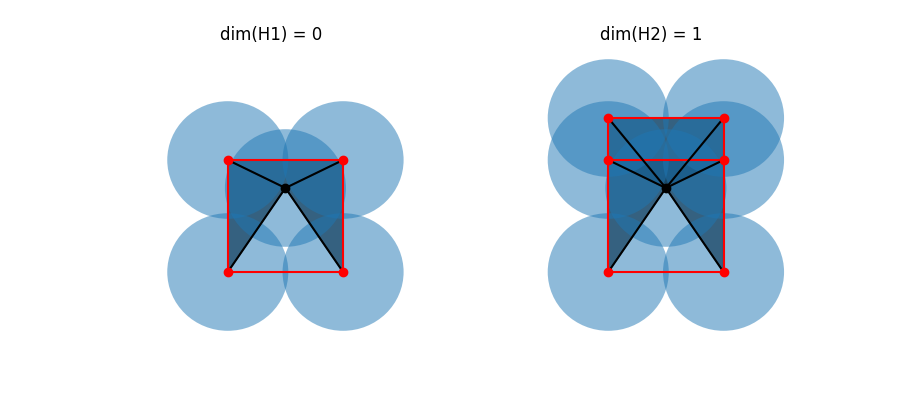
\includegraphics[scale=0.7]{figures/counter.png}
\end{figure}

\paragraph{Fake cycles}
Second, consider a situation in which $P^\delta$ covers $\D$ but there is an additional cycle in $\hom_1(Q^\delta)$ that does not reflect a feature of $\hom_1(\B)$.
In this case there is some point $x\in\D$ surrounded by this cycle that is covered by a point in $P\setminus Q$ but not $Q$.
The result is a non-zero element in $\hom_2(P^\delta, Q^\delta)$ that reflects the void containing this point and not the void corresponding to an element of $\hom_2(\D,\B)$, leading us to a false positive.
Fortunately, this situation is resolved by once again looking at the inclusion $(P^\delta, Q^\delta)\hookrightarrow (P^\gamma, Q^\gamma)$ as any such ``spurious'' cycles are killed for sufficiently large $\gamma > 0$.
This inclusion is contained in the inclusion of Rips complexes $\rips_\delta(P, Q)\hookrightarrow\rips_{2\gamma}(P, Q)$ as follows
\[ \rips_\delta(P, Q) \hookrightarrow \cech_\delta(P,Q)\hookrightarrow\cech_\gamma(P,Q)\hookrightarrow\rips_{2\gamma}(P, Q). \]

\subsection{What do we have? How can we use it?}

The components required to verify a network covers a bounded domain can be summarized by the following
\begin{enumerate}
    \item[a.] the boundary is adequately covered,
    \item[b.] the interior of the domain is covered.
\end{enumerate}
Condition (b) relies on condition (a) in order to provide a topological condition for \emph{coverage} that is necessary but not sufficient.
That is, it can verify coverage alone without false positives but may encounter false negatives.
In fact, the TCC tests a more specific problem: whether we have a reliable representation of the boundary \emph{and} a reliable representation of the interior.

As we have seen, this can be achieved by a collection of sensors that can detect the presence of neighboring sensors at two scales \emph{and} the presence of the boundary.
In reality, it is natural to assume we would like to confirm coverage of a domain in order to measure some quantity.
We therefore consider a situation in which sensors can measure some scalar value, representing a sample of a function defined on the domain.
By defining the boundary in terms of this function we no longer need to require that sensors can detect the presence of the boundary.
Specifically, we can replace the boundary of the domain with a sub-level set that resembles a boundary with specific topological properties.
The points close to the boundary can then be taken as the points measuring function values within a certain range.

In the following section we formalize the notion of a sub-level set resembling a boundary and state the conditions required to confirm coverage.
We then re-state the TCC as a condition that is both necessary \emph{and} sufficient for a more specific problem.% and show how it can be used to approximate the relative persistent homology of the function.
% Finally, we consider classes of functions which satisfy the assumptions made.
% Namely, we consider functions with multiple sub-level sets which may serve as a boundary for this procedure and show how they can be integrated to give a more robust signature for the function.


  \section{The Topological Coverage Criterion}
  % !TeX root = main.tex

\subsection{Assumptions}\label{ssec:assumptions}

We first generalize the notion of the topological boundary in the preceding example to the notion of a set which surrounds our domain.

Let $X\subset \R^d$ and $A\subset X$.
We say that $A$ \textbf{separates} $X$ if there exists a pair $(\I, \O)$ such that
\begin{itemize}
    \item $\I, A, \O$ are disjoint,
    \item $\I \cup \O = X\setminus A$,
    \item there is no path from $\I$ to $\O$ that does not cross $A$.
\end{itemize}

\begin{lemma}
    If $A$ separates $X$ with the pair $(\I, \O)$ then for all $k\geq 0$
    \[ \hom_k(\I)\cong\hom_k(\overline{A}, \O). \]
\end{lemma}
% \begin{proof}
%     If $A$ separates $X$ with the pair $(\I, \O)$ then $\I$ and $\O$ are not path connected and $\overline{A} = \I\cup\O$.
%
%     For all $k > 0$ suppose $[x]\in \hom_k(\overline{A}, \O)$ is non-trivial.
%     Because $\I$ and $\O$ are not path connected $\partial x \in C_{k-1}(\O)$ implies that $x\in C_k(\O)$ and therefore that $[x]$ is trivial in $\hom_k(\overline{A}, \O)$.
%     So $[x]$ is not a relative cycle and therefore $[x]\in \hom_k(\overline{A})$, $[x]\notin\hom_k(\O)$.
%     Because $\I$ and $\O$ are not path connected $[x]\notin\hom_k(\O)$ implies $[x]\in \hom_k(\overline{A}\setminus\O) = \hom_k(\I)$.
%
%     On the other hand, if $[x]\in \hom_k(\I)$ then $[x]\in \hom_k(\overline{A}, \I)$ as $\I\subset\overline{A}$ and, because $\I$ and $\O$ are not path connected, $[x]$ is trivial in $\hom_k(\overline{A}, \O)$ if and only if $[x]$ is trivial in $\hom_k(\I)$.
% \end{proof}

\begin{lemma}\label{lem:surrounds}
    If $A$ separates $X$ with the pair $(\I, \O)$ then for all $k\geq 0$, $\e > 0$
    \[\hom_k(\I\setminus A^\e)\cong \hom_k(\overline{A^\e}, \overline{\I^\e}).\]
\end{lemma}

We say that a subset $A$ \textbf{surrounds} $X$ if $A$ separates $\R^d$ with the pair $(X\setminus A, \overline{X})$.

\begin{lemma}\label{lem:surrounds}
    If $A$ surrounds $X$ then for all $\e > 0$
    \[\hom_0((\D\setminus\B^\e,\emptyset)\hookrightarrow (\overline{\B^\e}, \overline{\D^\e}))\]
    is an isomorphism.
\end{lemma}

\subsection{The Topological Coverage Criterion}

Let $\omega,\delta,\gamma \in \R$ such that $U_{\omega-2c\delta}$ is closed and surrounds $\D$, and $\gamma \geq 3\delta$ is such that we have the following sequence of inclusions
\[\D_{\omega - 2c\delta}\subset \D_{\omega - 2c\delta}^{2\delta} \subset \D_{\omega - 2c\delta}^{\delta + \gamma} \subset \D_{\omega + 2c\delta}.\]
In the following let $\B = \D_{\omega - 2c\delta}$.

Let $P$ be a finite subset of $\D$ and $Q = P\cap U_{\omega - c\delta}$.
We have the following commutative diagrams of inclusions between the pairs $(P,Q)$ and $(\D, \B)$ and their complements with increasing scale.

\[ \begin{tikzcd}
(P^\delta, Q^\delta) \arrow[hookrightarrow]{r}\arrow[hookrightarrow]{d}& (P^\gamma, Q^\gamma) \arrow[hookrightarrow]{d} \\%
(\D^{2\delta}, \B^{2\delta}) \arrow[hookrightarrow]{r} & (\D^{\delta+\gamma}, \B^{\delta+\gamma}),
\end{tikzcd}
\begin{tikzcd}
(\overline{\B^{\delta+\gamma}}, \overline{\D^{\delta+\gamma}})\arrow[hookrightarrow]{r}{j}\arrow[hookrightarrow]{d}& (\overline{\B^{2\delta}}, \overline{\D^{2\delta}}) \arrow[hookrightarrow]{d} \\%
(\overline{Q^\gamma}, \overline{P^\gamma}) \arrow[hookrightarrow]{r}{i} & (\overline{Q^\delta}, \overline{P^\delta}).
\end{tikzcd}\]

The following diagram is formed by applying the homology functor.
\[ \begin{tikzcd}\label{dgm:1}
\hom_0(\overline{\B^{\delta+\gamma}}, \overline{\D^{\delta+\gamma}})\arrow{r}{j_*}\arrow{d}& \hom_0(\overline{\B^{2\delta}}, \overline{\D^{2\delta}}) \arrow{d} \\%
\hom_0(\overline{Q^\gamma}, \overline{P^\gamma}) \arrow{r}{i_*} & \hom_0(\overline{Q^\delta}, \overline{P^\delta}).
\end{tikzcd}\]
Let $p_* : \im~j_*\to\im~i_*$.

\begin{theorem}[Geometric TCC]\label{thm:tcc}
    If $\im~\hom_k(\D_{\omega-2c\delta}\hookrightarrow \D_{\omega+{2c\delta}})\cong \hom_k(\D_{\omega - 2c\delta}^{2\delta})$ and $p_*$ is injective then $\D\setminus\D_{\omega-2c\delta}^{2\delta}\subseteq P^\delta$ and $Q^\delta$ separates $\D$.
\end{theorem}

\begin{corollary}
    If $\im~\hom_k(\D_{\omega-2c\delta}\hookrightarrow \D_{\omega+{2c\delta}})\cong \hom_k(\D_{\omega - 2c\delta}^{2\delta})$ and $p_*$ is injective then for all $k\geq 0$
    \[ \im~i_* \cong \hom_k(\D^{2\delta}, \B^{2\delta}).\]
\end{corollary}

% \begin{lemma}\label{lem:separate}
%     If $j_*$ is surjective and $p_*$ is injective then $Q^\delta$ separates $\D$.
% \end{lemma}
% \begin{proof}
%     Suppose, for the sake of contradiction, that $Q^\delta$ does not separate $\D$.
%     Then for all $(\I, \O)$ such that $\I \cup \O = \D\setminus Q^\delta$ there must exist some path from $\I$ to $\O$ that does not cross $Q^\delta$.
%     Formally, there exists a path $\pi : [0,1]\to\overline{Q^\delta}$ with $\pi(0)\in \I$ and $\pi(1)\in\O$.
%     Noting that $\overline{\B^{2\delta}}\subseteq \overline{Q^\delta}$ and, because $\overline{\B^{2\delta}} = \overline{\D^{2\delta}}\cup (\D\setminus\B^{2\delta})$ surrounds $\D^{2\delta}$ we can choose $(\I, \O)$ such that $\D\setminus \B^{2\delta}\subset \I$ and $\overline{\D^{2\delta}}\subset \O$.
%
%     Choose $x\in\D\setminus \B^{2\delta}$ and $y\in \overline{\D^{2\delta}}$ such that there exist paths $\pi_x : [0,1]\to \I$ with $\pi_x(0) = x$, $\pi_x(1) = \pi(0)$ and $\pi_y : [0,1]\to \O$ with $\pi_y(0) = y$, $\pi_y(1) = \pi(1)$.
%     $\pi_x, \pi_y$ and $\pi$ all generate chains in $C_1(\overline{Q^\delta}, \overline{P^\delta})$ and $\pi_x + \pi + \pi_y = \pi^*\in C_1(\overline{Q^\delta}, \overline{P^\delta})$ with $\partial\pi^* = x + y$.
%     Moreover, $y$ generates a chain in $C_0(\overline{P^\delta})$ as $\overline{\D^{2\delta}}\subseteq\overline{P^\delta}$.
%     So $x = \partial\pi^* + y$ is a relative boundary in $C_0(\overline{Q^\delta}, \overline{P^\delta})$ thus $[x] = 0 = [y]$ in $\hom_0(\overline{Q^\delta}, \overline{P^\delta})$ and therefore $[x] = [y]$ in $\im~i_*$.
%     However, because $\B^{2\delta}$ separates $\D$ with the pair $(\overline{\D^{2\delta}}, \D\setminus\B^{2\delta})$ we know that $[x]\neq [y]$ in $\hom_0(\overline{\B^{2\delta}}, \overline{\D^{2\delta}})\cong \im~j_*$, contradicting our assumption that $p_*$ is injective.
% \end{proof}
%
% In the following we will assume that $j_*$ is surjective and $p_*$ is injective.
% By Lemma~\ref{lem:separate} $Q^\delta$ separates $\D$ with a pair $(\I, \O)$.
% Let $\hat{Q}^\delta = Q^\delta \cup \O$, $\hat{P}^\delta = P^\delta \cup \O$ and $\hat{Q}^\gamma = Q^\gamma \cup \O$.
%
% \begin{lemma}
%     $\hom_*(\hat{P}^\delta, \hat{Q}^\delta)\cong \hom_*(P^\delta, Q^\delta)$ and $\hom_*(P^\delta\cup\hat{Q}^\gamma, \hat{Q}^\gamma)\cong \hom_*(P^\delta\cup Q^\gamma, Q^\gamma)$.
% \end{lemma}
% \begin{proof}
%     By the definition of $\hat{Q}^\delta$, $\hat{Q}^\gamma$ and $\O$ we have that $\hat{Q}^\delta\setminus\O = Q^\delta$ and $\hat{Q}^\gamma\setminus\O = Q^\gamma$ and $\cl~\O \subset \intr~\hat{Q}^\delta, \intr~\hat{Q}^\gamma$.
%     The desired results follow by Excision.
% \end{proof}
%
% \begin{lemma}
%     If $p_*$ is injective then $\B^{2\delta}\subseteq \hat{Q}^\gamma$.
% \end{lemma}
% \begin{proof}
%     Suppose $p_*$ is injective and there exists some $x\in \B^{2\delta}$ such that $x\notin \hat{Q}^\gamma$.
%     So there exists some $y\in U_{\omega - 2c\delta}$ such that $\dist(x, y) < 2\delta$.
%     Because $Q^\delta$ separates $\D = \O \cup Q^\delta \cup \I$ both $x$ and $y$ are either in $Q^\delta, \O$ or $\I$.
%     Moreover, $\overline{\I} = Q^\delta \cup \O = \hat{Q}^\delta$ so $\B^{2\delta}\cap\I = \B^{2\delta}\setminus \hat{Q}^\delta$ and $\B\cap\I = \B\setminus \overline{\I} = \B\setminus \hat{Q}^\delta = \emptyset$ as $\B\subset \hat{Q}^\delta$.
%     So $y\notin \I$ and, because $Q^\delta \subset Q^\gamma$ and $\O\subset \hat{Q}^\delta\subset\hat{Q}^\gamma$, we can assume w.l.o.g. that $x\in \B^{2\delta}\cap\I$.
%
%     If $y\in Q^\delta$ then there exists some $q\in Q$ such that $\dist(q, y) < \delta$ so
%     \[ \dist(q, x)\leq \dist(q, y) + \dist(x, y) < 3\delta\leq\gamma \]
%     which implies $x \in Q^\gamma$.
%
%     So we may assume that $y\in U_{\omega - 2c\delta}\cap\O$.
%     Because $Q^\delta$ separates $\D$ with $(\I, \O)$ there is no path from $x\in \I$ to $y\in\O$ that does not cross $Q^\delta$, so there must be some point $z\in Q^\delta$ in the shortest path from $x$ to $y$.
%     That is, there exists some $q\in Q$ such that $\dist(q, z) < \delta$ and $\dist(z, x) < \dist(x, y) < 2\delta$ so
%     \[ \dist(q, x)\leq \dist(q, z) + \dist(z, x) < \delta + 2\delta \leq \gamma. \]
%     So $y\in\O$ implies $x\in\hat{Q}^\gamma$.
%
% \end{proof}

  % !TeX root = main.tex

\subsection{Proof of the TCC}

\begin{lemma}\label{lem:jsurj}
    Given assumptions 1-3 the map $j_*$ is surjective.
\end{lemma}
\begin{proof}
    \textbf{TODO this true?
    What other conditions do we need for it to be true?
    Do we have to assume this as well?}
\end{proof}

\begin{lemma}\label{lem:psurj}
    Given assumptions 1-3, the map $p_*$ is surjective.
\end{lemma}
\begin{proof}
    \textbf{TODO Do we even need this?
    If $\im~i_*$ is finite-dimensional and $\rk~i_* \geq \rk~j_*$ is $p_*$ injective?
    We can also just state the theorem as ``if $p_*$ is injective.''}
\end{proof}
% \begin{proof}
%     By Lemma~\ref{lem:jsurj} $j_*$ is surjective.
%     Choose a basis for $\im~i_*$ such that each basis element is represented by a point in $P^\delta\setminus Q^\gamma$.
%     Let $x\in P^\delta\setminus Q^\gamma$ be such that $[x]$ is non-trivial in $\im~i_*$.
%     Suppose $x\in\B^{2\delta}$ and let $y\in\B$ such that $\dist(x, y)< 2\delta$.
%
%     First, suppose $y\in P^\delta$.
%     So there exists some $p\in P$ such that $\dist(p, y) < \delta$.
%     But $y\in \B = \D_{\omega-2c\delta}$ so $f(y)\leq \omega-2c\delta$.
%     Therefore, because $f$ is $c$-Lipschitz
%     \[ f(p) \leq c\dist(p, y) + f(y) < \omega - 2c\delta + c\delta = \omega - c\delta\]
%     so $p\in Q$, thus $y\in Q^\delta$.
%     So $y\in P^\delta$ implies $y\in Q^\delta$ and therefore, by contrapositive, $y\in\overline{Q^\delta}$ implies $y\in\overline{P^\delta}$.
%
%     Now, because $x\in\overline{Q^\gamma}$ by hypothesis $\dist(x, q) \geq \gamma$ for all $q\in Q$.
%     For any $z$ in the shortest path between $x$ and $y$ we have $\dist(x, z)\leq \dist(x, y) < 2\delta$, so the following inequality holds for all $q\in Q$
%     \begin{align*}
%         \dist(x, q) &\geq \dist(x, q) - \dist(x, z)\\
%         &> \gamma - 2\delta\\
%         &\geq \delta.
%     \end{align*}
%     So $z\in \overline{Q^\delta}$ for all $z$ in the shortest path from $x$ to $y$.
%     In particular, $x,y\in\overline{Q^\delta}$ therefore $y\in\overline{P^\delta}$.
%
%     Because $x,y\in\overline{Q^\delta}$ we have corresponding chain $x,y\in C_0(\overline{Q^\delta})$ and $y\in\overline{P^\delta}$ generates a chain $y\in C_0(P^\delta)$.
%     As we have shown that $x\in \B^{2\delta}$ implies that the shortest path from $x$ to $y$ is contained in $\overline{Q^\delta}$ there exists a path $h: [0,1]\to \overline{Q^\delta}$ with $h(0) = x$ and $h(1) = y$ that generates a chain $h\in C_1(\overline{Q^\delta})$.
%     So for $h\in C_1(\overline{Q^\delta}, \overline{P^\delta})$ with $\partial h = x + y$ we have that $x = \partial h + y$.
%     Thus $[x]$ is a relative boundary and is therefore trivial in $\hom_0(\overline{P^\delta}, \overline{Q^\delta})$, a contradiction, as we have assumed $[x]$ is non-trivial in $\im~i_*$.
%     So we may conclude that $x\notin \B^{2\delta}$.
%
%     So $x\in\overline{\B^{2\delta}}$ and $x\in \D\setminus\B^{2\delta}$.
%     So $[x]$ is non-trivial in $\hom_0(\overline{\B^{2\delta}},\overline{\D^{2\delta}})$ and, because $j_*$ is surjective, $\im~j_* = \hom_0(\overline{\B^{2\delta}},\overline{\D^{2\delta}})$.
%     So $p_*$ is surjective as $p_*[x] = [x]\in\im~p_*$ for all non-trivial $[x]\in\im~i_*$.
% \end{proof}

\begin{lemma}\label{lem:coverage}
    Given assumptions 1-3, if $p_*$ is injective then $\D\setminus\B^{2\delta}\subseteq P^\delta$.
\end{lemma}
\begin{proof}
    Suppose, for the sake of contradiction, that $p_*$ is injective and there exists a point $x\in (\D\setminus\B^{2\delta})\setminus P^\delta$.
    So $[x]$ is non-trivial in $\hom_0(\overline{\B^{2\delta}},\overline{\D^{2\delta}}) = \im~j_*$ as $x$ is in some connected component of $\D\setminus\B^{2\delta}$ and $j_*$ is surjective.
    So we have the following sequence of maps induced by inclusions
    \[ \hom_0(\overline{\B^{2\delta}},\overline{\D^{2\delta}})\xrightarrow{f_*} \hom_0(\overline{\B^{2\delta}},\overline{\D^{2\delta}}\cup\{x\})\xrightarrow{g_*} \hom_0(\overline{Q^\delta},\overline{P^\delta}).\]
    As $f_*[x]$ is trivial in $\hom_0(\overline{\B^{2\delta}},\overline{\D^{2\delta}}\cup\{x\})$ we have that $p_*[x] = (g_*\circ f_*)[x]$ is trivial, contradicting our hypothesis that $p_*$ is injective.
\end{proof}

\begin{lemma}\label{lem:separate}
    Given assumptions 1-3, if the map $p_*$ is injective then $Q^\delta$ separates $\D$.
\end{lemma}
\begin{proof}
    Suppose, for the sake of contradiction, that $Q^\delta$ does not separate $\D$.
    Then for all $(\I, \O)$ such that $\I \cup \O = \D\setminus Q^\delta$ there must exist some path from $\I$ to $\O$ that does not cross $Q^\delta$.
    Formally, there exists a path $\pi : [0,1]\to\overline{Q^\delta}$ with $\pi(0)\in \I$ and $\pi(1)\in\O$.
    Noting that $\overline{\B^{2\delta}}\subseteq \overline{Q^\delta}$ and, because $\overline{\B^{2\delta}} = \overline{\D^{2\delta}}\cup (\D\setminus\B^{2\delta})$ surrounds $\D^{2\delta}$ we can choose $(\I, \O)$ such that $\D\setminus \B^{2\delta}\subset \I$ and $\overline{\D^{2\delta}}\subset \O$.

    Choose $x\in\D\setminus \B^{2\delta}$ and $y\in \overline{\D^{2\delta}}$ such that there exist paths $\pi_x : [0,1]\to \I$ with $\pi_x(0) = x$, $\pi_x(1) = \pi(0)$ and $\pi_y : [0,1]\to \O$ with $\pi_y(0) = y$, $\pi_y(1) = \pi(1)$.
    $\pi_x, \pi_y$ and $\pi$ all generate chains in $C_1(\overline{Q^\delta}, \overline{P^\delta})$ and $\pi_x + \pi + \pi_y = \pi^*\in C_1(\overline{Q^\delta}, \overline{P^\delta})$ with $\partial\pi^* = x + y$.
    Moreover, $y$ generates a chain in $C_0(\overline{P^\delta})$ as $\overline{\D^{2\delta}}\subseteq\overline{P^\delta}$.
    So $x = \partial\pi^* + y$ is a relative boundary in $C_0(\overline{Q^\delta}, \overline{P^\delta})$ thus $[x] = 0 = [y]$ in $\hom_0(\overline{Q^\delta}, \overline{P^\delta})$ and therefore $[x] = [y]$ in $\im~i_*$.
    However, because $\B^{2\delta}$ separates $\D$ with the pair $(\overline{\D^{2\delta}}, \D\setminus\B^{2\delta})$ we know that $[x]\neq [y]$ in $\hom_0(\overline{\B^{2\delta}}, \overline{\D^{2\delta}})\cong \im~j_*$, contradicting our assumption that $p_*$ is injective.
\end{proof}

\begin{theorem}[Geometric TCC]\label{thm:tcc}
    Let $\D\subset\R^d$ and $f:\D\to\R$ be a $c$-Lipschitz function satisfying assumptions 1-3 for $\omega\in\R$, $\delta > 0$, and $\gamma > 3\delta$.
    Let $P\subset\D$ be a collection of sensors and let $Q = P\cap \D_{\omega - c\delta}$, $\B = \D_{\omega - 2c\delta}$.
    Let $p_* : \im~j_*\to\im~i_*$ for $j_*$, $i_*$ as defined in Diagram~\ref{dgm:1}.

    If $\rk~i_*\geq \rk~j_*$ then $\D\setminus\B^{2\delta}\subseteq P^\delta$ and $Q^\delta$ separates $\D$.
\end{theorem}
\begin{proof}
    % Lemma~\ref{lem:psurj} states that $p_*$ is surjective so $p_*$ is surjective, so $\rk~i_*\leq \rk~j_*$.
    % Because $\rk~i_*\geq \rk~j_*$, $$\rk~i_* = \rk~j_*$.
    Because $P$ is a finite point set we know that $\im~i_*$ is finite-dimensional.
    Because $\rk~i_*\geq \rk~j_*$ $j_*$ is finite dimensional as well so $p_*$ is injective.
    Therefore $\D\setminus\B^{2\delta}\subseteq P^\delta$ by Lemma~\ref{lem:coverage} and $Q^\delta$ separates $\D$ by Lemma~\ref{lem:separate}.
\end{proof}

  % !TeX root = main.tex

\subsection{Proof of the Interleaving}

In the following we will assume that $j_*$ is surjective and $p_*$ is injective.
By Lemma~\ref{lem:separate} $Q^\delta$ separates $\D$ with a pair $(\I, \O)$.
Let $\hat{Q}^\delta = Q^\delta \cup \O$, $\hat{P}^\delta = P^\delta \cup \O$ and $\hat{Q}^\gamma = Q^\gamma \cup \O$.

\begin{lemma}
    $\hom_*(\hat{P}^\delta, \hat{Q}^\delta)\cong \hom_*(P^\delta, Q^\delta)$ and $\hom_*(P^\delta\cup\hat{Q}^\gamma, \hat{Q}^\gamma)\cong \hom_*(P^\delta\cup Q^\gamma, Q^\gamma)$.
\end{lemma}
\begin{proof}
    By the definition of $\hat{Q}^\delta$, $\hat{Q}^\gamma$ and $\O$ we have that $\hat{Q}^\delta\setminus\O = Q^\delta$ and $\hat{Q}^\gamma\setminus\O = Q^\gamma$ and $\cl~\O \subset \intr~\hat{Q}^\delta, \intr~\hat{Q}^\gamma$.
    The desired results follow by Excision.
\end{proof}

\begin{lemma}\label{lem:qcontain}
    If $p_*$ is injective then $\B^{2\delta}\subseteq \hat{Q}^\gamma$.
\end{lemma}
\begin{proof}
    Suppose $p_*$ is injective and there exists some $x\in \B^{2\delta}$ such that $x\notin \hat{Q}^\gamma$.
    So there exists some $y\in U_{\omega - 2c\delta}$ such that $\dist(x, y) < 2\delta$.
    Because $Q^\delta$ separates $\D = \O \cup Q^\delta \cup \I$ both $x$ and $y$ are either in $Q^\delta, \O$ or $\I$.
    Moreover, $\overline{\I} = Q^\delta \cup \O = \hat{Q}^\delta$ so $\B^{2\delta}\cap\I = \B^{2\delta}\setminus \hat{Q}^\delta$ and $\B\cap\I = \B\setminus \overline{\I} = \B\setminus \hat{Q}^\delta = \emptyset$ as $\B\subset \hat{Q}^\delta$.
    So $y\notin \I$ and, because $Q^\delta \subset Q^\gamma$ and $\O\subset \hat{Q}^\delta\subset\hat{Q}^\gamma$, we can assume w.l.o.g. that $x\in \B^{2\delta}\cap\I$.

    If $y\in Q^\delta$ then there exists some $q\in Q$ such that $\dist(q, y) < \delta$ so
    \[ \dist(q, x)\leq \dist(q, y) + \dist(x, y) < 3\delta\leq\gamma \]
    which implies $x \in Q^\gamma$.

    So we may assume that $y\in U_{\omega - 2c\delta}\cap\O$.
    Because $Q^\delta$ separates $\D$ with $(\I, \O)$ there is no path from $x\in \I$ to $y\in\O$ that does not cross $Q^\delta$, so there must be some point $z\in Q^\delta$ in the shortest path from $x$ to $y$.
    That is, there exists some $q\in Q$ such that $\dist(q, z) < \delta$ and $\dist(z, x) < \dist(x, y) < 2\delta$ so
    \[ \dist(q, x)\leq \dist(q, z) + \dist(z, x) < \delta + 2\delta \leq \gamma. \]
    So $y\in\O$ implies $x\in\hat{Q}^\gamma$.

\end{proof}

The following lemma is a well-established result that we provide without proof.

\begin{lemma}[Lemma 3.2 from~\cite{chazal08towards}]\label{lem:sandwich}
    Given a sequence $A\to B\to C\to D\to E\to F$ of homomorphisms between finite-dimensional vector spaces, if $\rk(A\to F) = \rk(C\to D)$ then this quantity also equals the rank of $B\to E$.
    Similarly, if $A\to B\to C\to E\to F$ is a sequence of homomorphisms such that $\rk(A\to F) = \dim~C$ then $\rk(B\to E) = \dim~C$.
\end{lemma}

% \begin{lemma}
%     If $p_*$ is injective then $\im~\hom_*(P^\delta\to (P^\delta\cup \hat{Q}^\gamma)\setminus\B)\cong \hom_*(\D\setminus\B^{2\delta})$.
% \end{lemma}
% \begin{proof}
%     \textbf{TODO requires \[ \D\setminus \B^{2\delta} \subseteq P^\delta \subseteq P^\delta \cup U_{\omega - 2c\delta}^{2\delta}\subseteq P^\delta\cup \hat{Q}^\gamma \subseteq \D \] and $\im~\hom_*(\D\setminus \B^{2\delta} \to \D)\cong\hom_*(P^\delta \cup U_{\omega - 2c\delta}^{2\delta}) = \hom_*(\D)$.}
% \end{proof}
% % \begin{proof}
% %     First note that because $p_*$ is injective $\D\setminus\B^{2\delta}\subseteq P^\delta$ and because $\B^{2\delta}\subseteq U_\omega$ we have $\D\setminus U_\omega \subseteq \D\setminus \B^{2\delta} \subseteq P^\delta$.
% %     We have the following sequence of inclusions
% %     \[ \D\setminus U_\omega \subseteq P^\delta \subseteq P^\delta \cup U_{\omega - 2c\delta}^{2\delta}\subseteq P^\delta\cup \hat{Q}^\gamma \subseteq \D \]
% %     which induces the following sequence of homomorphisms
% %     \[ \hom_*(\D\setminus U_\omega)\to\hom_*(P^\delta\setminus\B)\to\hom_*((P^\delta \cup \B^{2\delta})\setminus \B)\to\hom_*((P^\delta\cup\hat{Q}^\gamma)\setminus\B)\to\hom_*(\D\setminus\B).\]
% %     As $\D\setminus\B^{2\delta}\subseteq P^\delta$ implies $P^\delta\cup\B^{2\delta} = \D$ and $\hom_*(\D\setminus U_\omega)\cong \hom_*(\D\setminus \B)$ we have that $\im~\hom_*(\D\setminus U_\omega\to \D\setminus \B)\cong \hom_*(\D\setminus\B)$ and therefore $\im~\hom_*(P^\delta\to(P^\delta\cup\hat{Q}^\gamma)\setminus\B)\cong\hom_*(\D\setminus \B)$ by Lemma~\ref{lem:sandwich}.
% % \end{proof}

\begin{lemma}
    Given assumptions 1-3, if $p_*$ is injective then $\im~\hom_*(\hat{Q}^\delta \to \hat{Q}^{\gamma})\cong \hom_*(\B^{2\delta}).$
\end{lemma}
\begin{proof}
    By assumption 3 $\D_{\omega-c\delta}^\delta\to \D_{\omega-2c\delta}^{2\delta}$ is a deformation retraction so $\hom_*(\D_{\omega-c\delta}^\delta)\to \hom_*(\D_{\omega-2c\delta}^{2\delta})$ is an isomorphism.
    As $Q = P\cap \D_{\omega-c\delta}$ we have that $\hat{Q}^\delta\subset \D_{\omega-c\delta}^\delta$ and $\hat{Q}^\gamma\subset\D_{\omega - c\delta}^\gamma\subset \D_{\omega + 2c\delta}$ by assumption 4.
    If $p_*$ is injective we know that $\D_{\omega - 2c\delta}^{2\delta}\subseteq \hat{Q}^\gamma$ by Lemma~\ref{lem:qcontain} so we have the following sequence of homomorphisms
    \[ \hom_*(\D_{\omega - 2c\delta})\to \hom_*(\hat{Q}^\delta)\to \hom_*(\D_{\omega-c\delta}^\delta)\to \hom_*(\D_{\omega - 2c\delta}^{2\delta})\to\hom_*(\hat{Q}^\gamma)\to\hom_*(\D_{\omega + 2c\delta}).\]
    By assumption 2 $\im~\hom_*(\D_{\omega - 2c\delta}\hookrightarrow U_{\omega+2c\delta})\cong\hom_*(U_{\omega-2c\delta}^{2\delta})$ so \[\hom_*(\hat{Q}^\delta\hookrightarrow\hat{Q}^\gamma)\cong\hom_*(\D_{\omega-c\delta}^\delta\to \D_{\omega-2c\delta}^{2\delta})\cong \hom_*(\B^{2\delta})\] by Lemma~\ref{lem:sandwich}.
\end{proof}

\begin{lemma}
    Given assumption 2, if $p_*$ is injective then $\im~\hom_*(P^\delta\setminus \B^{2\delta} \to P^\delta\setminus \B)\cong \hom_*(\D\setminus\B^{2\delta}).$
\end{lemma}
\begin{proof}
    If $p_*$ is injective we have the following sequence of homomorphisms induced by inclusion
    \[\hom_*(\D\setminus\D_{\omega+2c\delta})\to\hom_*(P^\delta\setminus \B^{2\delta})\to\hom_*(\D\setminus\B^{2\delta})\to\hom_*(P^\delta\setminus \B)\to\hom_*(\D\setminus\B).\]
    By assumption 2 $\hom_*(\D\setminus\D_{\omega+2c\delta}\hookrightarrow \D\setminus\B)\cong\hom_*(\D\setminus\B^{2\delta})$ so $\im~\hom_*(P^\delta\setminus \B^{2\delta} \to P^\delta\setminus\B)\cong \hom_*(\D\setminus\B^{2\delta})$ by Lemma~\ref{lem:sandwich}.
\end{proof}


\section{Future Work}

Conformation of the TCC implies that we cover the interior of the domain $\D\setminus\B^{2\delta}$ and that $Q^\delta$ separates $\D$ which.
As we have shown, this implies that the inclusion our sampled boundary at scales $\delta,\gamma$ captures the homology of the thickened boundary $\B^{2\delta}$ and the inclusion of our sampled interior captures the homology of the interior $\D\setminus\B^{2\delta}$.
However, this alone does not imply that the inclusion of pairs $(P^\delta, Q^\delta)\to (P^\gamma, Q^\gamma)$ captures the \emph{relative} homology of the pair $(\D,\B^{2\delta})$ as it does not account for homological features that may appear only in relative homology.
Specifically, any principal homology classes in $\hom_*(\D)$ that become relative homology classes in $\hom_*(\D\setminus\B^{2\delta}, \D_{\omega +2c\delta}\setminus \B^{2\delta})$ may not occur \emph{at all} in $\hom_*(P^\delta, Q^\delta)$.
Identifying additional assumptions or side-effects of the TCC is the subject of future work, and would allow us to prove Lemma~\ref{lem:broken} and Theorem~\ref{thm:scalar}.

% , as we have shown, implies that $\B^{2\delta}\subset Q^\delta$ and the inclusions $\hom_*(\hat{Q}^\delta\hookrightarrow\hat{Q}^\gamma)$ and $\im~\hom_*(P^\delta\setminus \B^{2\delta} \to P^\delta\setminus \B)$ are isomorphic to $\hom_*(\B^{2\delta})$ and $\hom_*(\D\setminus\B^{2\delta})$ respectively.
% That is, the inclusion of our sampled boundary serv

% \begin{lemma}
%     If $\im~\hom_*(\hat{Q}^\delta\to\hat{Q}^\gamma)\cong\hom_*(\B^{2\delta})$ and $\im~\hom_*(P^\delta\setminus\B\to (P^\delta\cup \hat{Q}^\gamma)\setminus\B)\cong \hom_*(\D\setminus\B^{2\delta})$ then
%     \[\im~\hom_*((P^\delta, Q^\delta)\to (P^\delta\cup Q^\gamma, Q^\gamma))\cong \hom_*(\D, \B). \]
% \end{lemma}

\begin{lemma}~\label{lem:broken}
    If $\im~\hom_*(\hat{Q}^\delta\to\hat{Q}^\gamma)\cong\hom_*(\B^{2\delta})$ and $\im~\hom_*(P^\delta\setminus Q^\gamma \to P^\delta\setminus Q^\delta)\cong \hom_*(\D\setminus\B^{2\delta})$ then
    \[\im~\hom_*((P^\delta, Q^\delta)\to (P^\delta\cup Q^\gamma, Q^\gamma))\cong \hom_*(\D^{2\delta}, \B^{2\delta}). \]
\end{lemma}

\begin{theorem}\label{thm:scalar}
    If $\im~\hom_*((P^\delta, Q^\delta)\to (P^\delta\cup Q^\gamma, Q^\gamma))\cong \hom_*(\D^{2\delta}, \B^{2\delta})$ then \[\{(P_\alpha^\delta, Q^\delta)\to (P_\alpha^\delta\cup Q^\gamma, Q^\gamma)\}_{\alpha > \omega+2c\delta}\] is $c\delta$-interleaved with $\{(\D_\alpha, \B^{2\delta})\}_{\alpha > \omega +2c\delta}$.
\end{theorem}

  % % !TeX root = ../main.tex

\begin{frame}
  \frametitle{Relative Homology and The TCC}

  \begin{itemize}
    \item Relative homology and separation,
    \item Properties of surrounding pairs,
    \item Assumption 1 and The Geometric TCC,
    \item Duality, Assumption 2, and the Algorithmic TCC.
  \end{itemize}
\end{frame}

\begin{frame}
  \frametitle{Relative Homology and Separation}

  \begin{itemize}
    \item The idea of relative homology
    \item relative homology of separated sets
  \end{itemize}

\end{frame}

\begin{frame}
  \frametitle{Properties of Surrounding Pairs}

  % \begin{itemize}
  %   \item surrounding pairs
  %   \item Coverage Lemma.
  %   \item Goal: show $\ell$ injective.
  % \end{itemize}

  \only<1>{\begin{definition}[Surrounding Pair]
    Let $X$ be a topological space and $(D,B)$ a pair in $X$.
    The set $B$ \textbf{surrounds $D$ in $X$} if $B$ separates $X$ with the pair $(D\setminus B, X\setminus D)$.
    We will refer to such a pair as a \textbf{surrounding pair in $X$}.
  \end{definition}}

  \only<2>{\begin{lemma}\label{lem:coverage}
    Let $(D, B)$ be a surrounding pair in $X$ and $U\subseteq D$, $V\subseteq U\cap B$ be subsets.
    Let $\ell: \hom_0(X\setminus B, X\setminus D)\to \hom_0(X\setminus V, X\setminus U)$ be induced by inclusion.

    If $\ell$ is injective then $D\setminus B\subseteq U$ and $V$ surrounds $U$ in $D$.
  \end{lemma}}
\end{frame}

\begin{frame}
  \frametitle{{\small Assumption 1 and the Geometric TCC}}
  \begin{small}
    Compact $D\subset\X$, $c$-Lipschitz $f : D\to\R$.\\
    $\omega\in\R$ such that $\B := f^{-1}((-\infty, \omega])$ surrounds $D$ in $\X$.\\
    Finite collection of points $P\subset D$, $Q_\alpha := P\cap B_\alpha$ for $\alpha\in\R$.\\
    Constants $\zeta\geq\delta > 0$.
  \end{small}

  % \begin{itemize}
  %   \item Rank lemma
  %   \item Diagrams and Assumption 1
  %   \item statement of the Geometric TCC
  % \end{itemize}

  \begin{lemma}\label{lem:psurj}
    Let $i : \hom_0(\overline{Q_{\omega+c\delta}^\delta}, \overline{P^\delta})\to \hom_0(\overline{Q_{\omega-c\zeta}^\delta}, \overline{P^\delta})$.

    If $B_\omega$ surrounds $D$ in $\X$ then $\mathbf{dim}~\hom_0(\overline{B_\omega}, \overline{D})\geq \mathbf{rk}~i$.
  \end{lemma}

  % \begin{equation}\label{dgm:1}
  % \begin{tikzcd}
  %   (P^\delta, Q_{\omega-c\zeta}^\delta) \arrow[hookrightarrow]{r}\arrow[hookrightarrow]{d} &
  %   (P^\delta, Q_{\omega+c\delta}^\delta) \arrow[hookrightarrow]{d} \\
  %   %
  %   (D, B_\omega) \arrow[hookrightarrow]{r} &
  %   (D, B_{\omega+c(\delta+\zeta)}),
  % \end{tikzcd}
  % \begin{tikzcd}
  %   \hom_0(\overline{B_{\omega+c(\delta+\zeta)}},\overline{D})\arrow{d}{m} \arrow{r}{j} &
  %   \hom_0(\overline{B_\omega}, \overline{D}) \arrow{d}{\ell} \\
  %   %
  %   \hom_0(\overline{Q_{\omega+c\delta}^\delta}, \overline{P^\delta}) \arrow{r}{i} &
  %   \hom_0(\overline{Q_{\omega-c\zeta}^\delta}, \overline{P^\delta}).
  % \end{tikzcd}\end{equation}
\end{frame}

\begin{frame}
  \frametitle{{\small Assumption 1 and the Geometric TCC}}

  % \begin{equation}\label{dgm:1}
  % \begin{tikzcd}
  %   (P^\delta, Q_{\omega-c\zeta}^\delta) \arrow[hookrightarrow]{r}\arrow[hookrightarrow]{d} &
  %   (P^\delta, Q_{\omega+c\delta}^\delta) \arrow[hookrightarrow]{d} \\
  %   %
  %   (D, B_\omega) \arrow[hookrightarrow]{r} &
  %   (D, B_{\omega+c(\delta+\zeta)}),
  % \end{tikzcd}
  % \begin{tikzcd}
  %   \hom_0(\overline{B_{\omega+c(\delta+\zeta)}},\overline{D})\arrow{d}{m} \arrow{r}{j} &
  %   \hom_0(\overline{B_\omega}, \overline{D}) \arrow{d}{\ell} \\
  %   %
  %   \hom_0(\overline{Q_{\omega+c\delta}^\delta}, \overline{P^\delta}) \arrow{r}{i} &
  %   \hom_0(\overline{Q_{\omega-c\zeta}^\delta}, \overline{P^\delta}).
  % \end{tikzcd}\end{equation}
  \begin{textblock*}{11cm}(1cm,2cm)
    \textbf{Assumption 1}\\ $\hom_0(D\setminus B_{\omega+c(\delta+\zeta)}\hookrightarrow D\setminus B_\omega)$ is \emph{surjective}.
  \end{textblock*}

  \begin{textblock*}{11cm}(1cm,4.5cm)
    % 
\includegraphics[trim=50 190 0 200, clip, scale=0.2]{scripts/figures/scalar.png}
    % 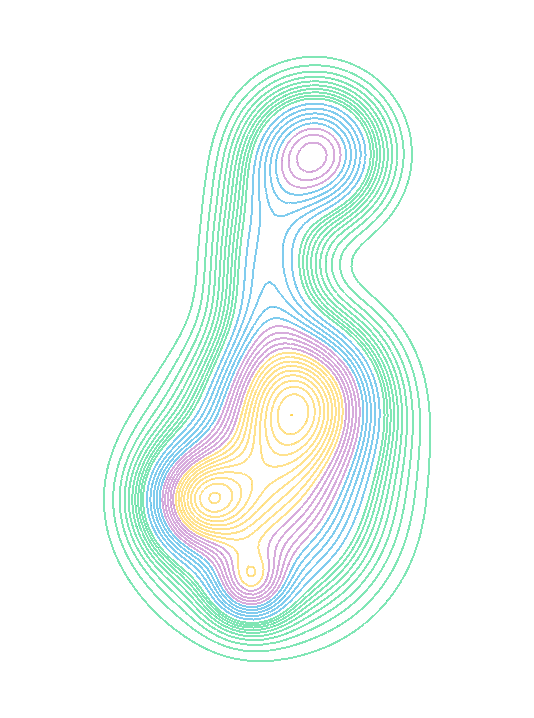
\includegraphics[trim=100 25 75 0, clip, angle=280, scale=0.25]{scripts/figures/scalar_contour.png}
    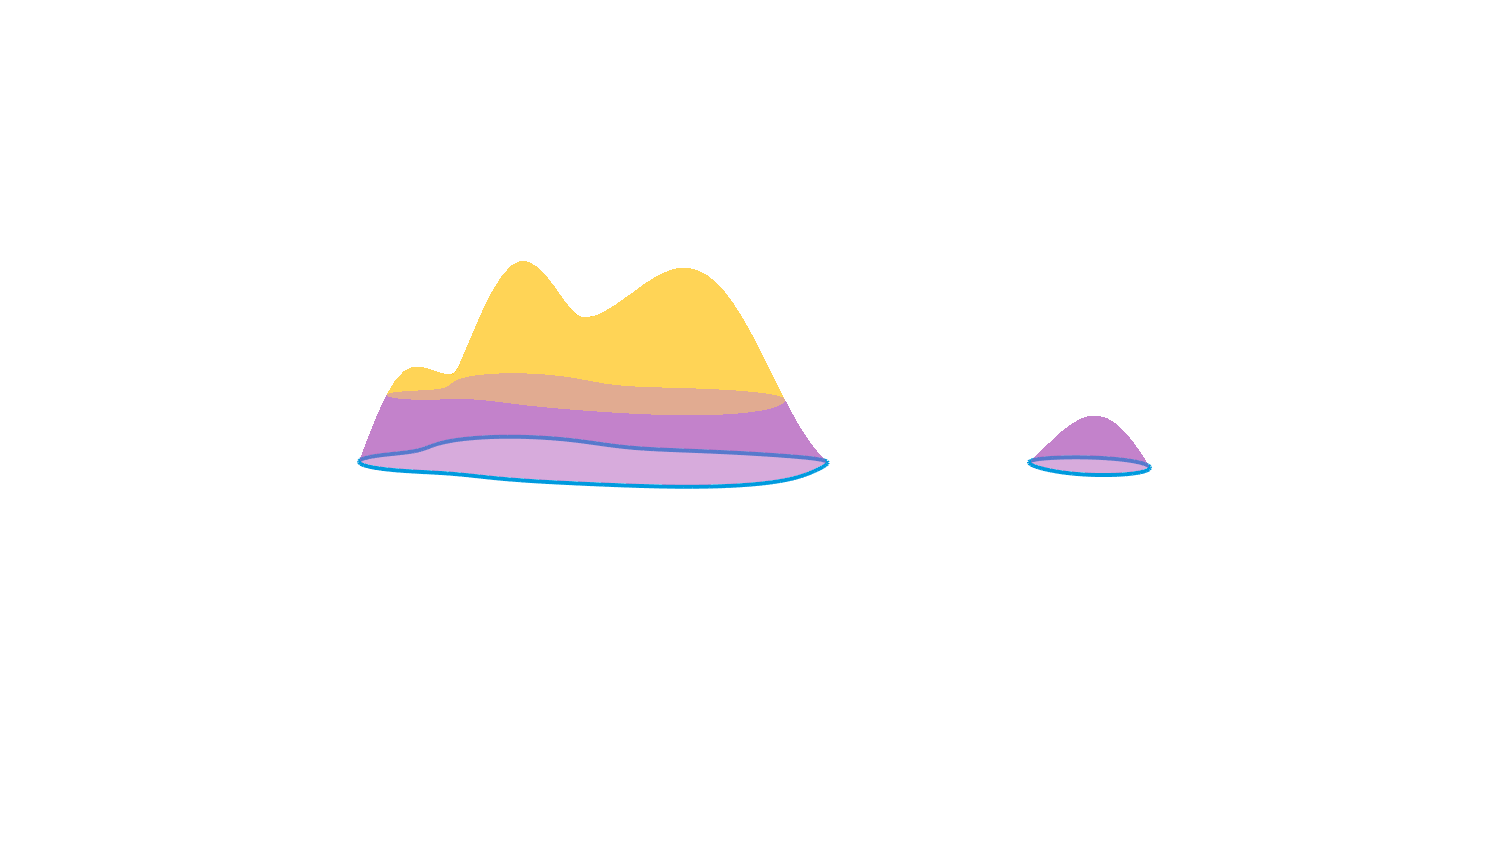
\includegraphics[trim=200 300 200 200, clip, width=0.5\textwidth]{../scripts/figures/surf/ass1_C_side.png}
    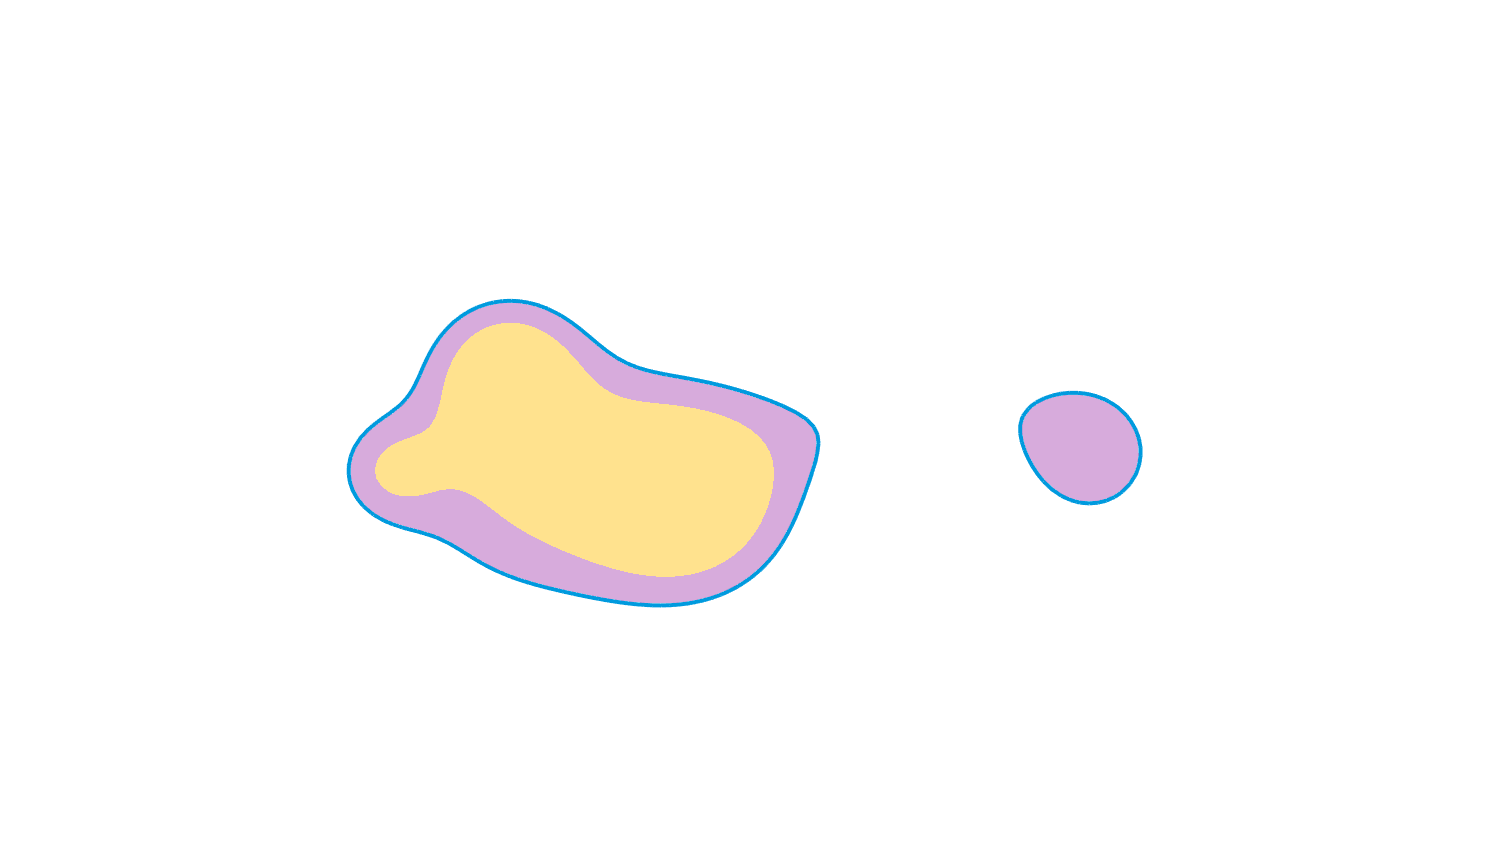
\includegraphics[trim=300 150 200 200, clip, width=0.3\textwidth]{../scripts/figures/surf/ass1_C_top.png}
    
\includegraphics[trim=200 300 200 200, clip, width=0.5\textwidth]{../scripts/figures/surf/ass1_D_side.png}
    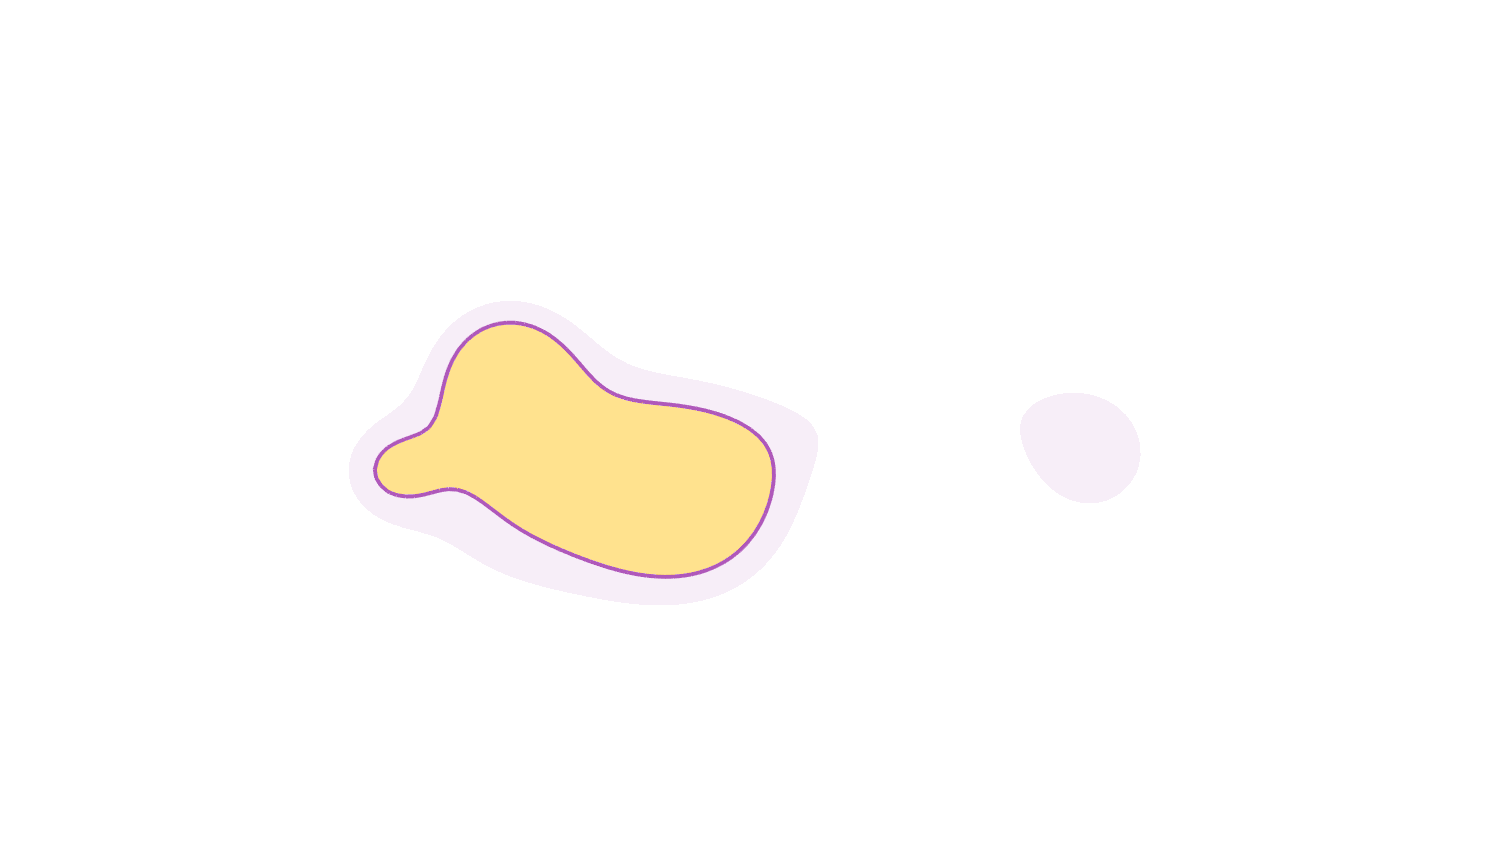
\includegraphics[trim=300 150 200 200, clip, width=0.3\textwidth]{../scripts/figures/surf/ass1_D_top.png}
    % 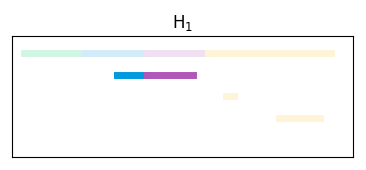
\includegraphics[scale=0.7]{scripts/figures/scalar_barcode_H1-masked.png}
  \end{textblock*}
\end{frame}

\begin{frame}
  \frametitle{{\small Assumption 1 and the Geometric TCC}}

  % \[\begin{tikzcd}
  %   \hom_0(\overline{B_{\omega+c(\delta+\zeta)}},\overline{D})\arrow{d}{m} \arrow{r}{j} &
  %   \hom_0(\overline{B_\omega}, \overline{D}) \arrow{d}{\ell} \\
  %   %
  %   \hom_0(\overline{Q_{\omega+c\delta}^\delta}, \overline{P^\delta}) \arrow{r}{i} &
  %   \hom_0(\overline{Q_{\omega-c\zeta}^\delta}, \overline{P^\delta}).
  % \end{tikzcd}\]

  \begin{theorem}[Geometric TCC]
    % Let $j : \hom_0(\cmp{B_{\omega+c(\delta+\zeta)}},\cmp{D})\to \hom_0(\cmp{\B},\cmp{D})$ and $i : \hom_0(\cmp{\QQ^\of}, \cmp{P^\of})\to \hom_0(\cmp{\Q^\of}, \cmp{P^\of})$ be induced by inclusion.
    %
    If $j$ is surjective and $\mathbf{rk}~i\geq \mathbf{rk}~j$ then $D\setminus B_\omega\subseteq P^\delta$ and $Q_{\omega-c\zeta}^\delta$ surrounds $P^\delta$ in $D$.
  \end{theorem}
\end{frame}

\begin{frame}
  \frametitle{{\small Duality, Assumption 2, and the Algorithmic TCC}}

  % \begin{itemize}
  %   \item Can't compute homology of complements: duality
  %   \item don't know number of connected components: assumption 2
  %   \item Rips-\v Cech interleaving and the Algorithmic TCC
  % \end{itemize}

  \textbf{Duality:} $\hom_d(P^\e,Q_z^\e)\cong\hom_0(D\setminus Q_z^\e, D\setminus P^\e)$.

  % \begin{textblock*}{12cm}(1cm,4.5cm)
  %
  % \end{textblock*}
\end{frame}


\begin{frame}
  \frametitle{{\small Duality, Assumption 2, and the Algorithmic TCC}}

  % \begin{itemize}
  %   \item Can't compute homology of complements: duality
  %   \item don't know number of connected components: assumption 2
  %   \item Rips-\v Cech interleaving and the Algorithmic TCC
  % \end{itemize}

  \only<1>{\begin{textblock*}{11cm}(1cm,2cm)
    \textbf{Assumption 2:} $\hom_0(D\setminus B_\omega\hookrightarrow D\setminus B_{\omega-c(\delta+\zeta)})$ is \emph{injective}.
  \end{textblock*}}

  \begin{textblock*}{12cm}(1cm,4.5cm)
    \includegraphics<1>[trim=200 300 200 200, clip, width=0.5\textwidth]{../scripts/figures/surf/ass2_C_side.png}
    \includegraphics<1>[trim=300 200 200 200, clip, width=0.3\textwidth]{../scripts/figures/surf/ass2_C_top.png}
    \includegraphics<1>[trim=200 300 200 200, clip, width=0.5\textwidth]{../scripts/figures/surf/ass2_B_side.png}
    \includegraphics<1>[trim=300 200 200 200, clip, width=0.3\textwidth]{../scripts/figures/surf/ass2_B_top.png}
  \end{textblock*}

  \only<2>{\begin{lemma}\label{lem:assumption2}
    If $\hom_0(D\setminus B_\omega\hookrightarrow D\setminus B_{\omega+c(\delta+\zeta)})$ is injective and each component of $D\setminus B_\omega$ contains a point in $P$ then $\mathbf{dim}~\hom_0(\rips^\delta(P\setminus Q_{\omega-c\zeta})) \geq \mathbf{dim}~\hom_0(D\setminus B_\omega)$.
  \end{lemma}}
\end{frame}

\begin{frame}
  \frametitle{{\small Duality, Assumption 2, and the Algorithmic TCC}}

  % \begin{itemize}
  %   \item Can't compute homology of complements: duality
  %   \item don't know number of connected components: assumption 2
  %   \item Rips-\v Cech interleaving and the Algorithmic TCC
  % \end{itemize}
  \begin{small}
    \[ \hom_k(\rips^\e(P, Q_w))\xrightarrow{J_w^\e}\hom_k(\cech^\e(P, Q_w))\xrightarrow{I_w^\e}\hom_k(\rips^\e(P, Q_w))\]
    % so
    % \[\mathbf{rk}~\hom_d(\cech^{\delta}(P, Q_{\omega-c\zeta})\hookrightarrow\cech^{\delta}(P, Q_{\omega+c\delta})) \geq\mathbf{rk}~ \hom_d(\rips^{\delta}(P, Q_{\omega-c\zeta})\hookrightarrow\rips^{2\delta}(P, Q_{\omega+c\delta}))\]

    \begin{theorem}[Algorithmic TCC]\label{thm:algo_tcc}
      Suppose $\hom_0(D\setminus B_{\omega+c(\delta+\zeta)}\hookrightarrow D\setminus B_\omega)$ is surjective and $\hom_0(D\setminus B_\omega\hookrightarrow D\setminus B_{\omega-c(\delta+\zeta)})$ is injective.

       If $\mathbf{rk}~\hom_d(\rips^\delta(P, Q_{\omega -c\zeta})\hookrightarrow \rips^{2\delta}(P, Q_{\omega+c\delta})) \geq \mathbf{dim}~\hom_0(\rips^\delta(P\setminus Q_{\omega-c\zeta}))$ then $D\setminus B_\omega\subseteq P^\delta$ and $Q_{\omega-c\zeta}^\delta$ surrounds $P^\delta$ in $D$.
    \end{theorem}
  \end{small}

  % \begin{textblock*}{12cm}(1cm,4.5cm)
  %
  % \end{textblock*}
\end{frame}

  % % \input{excision}
  % \input{stability}
  % \input{sampling}
  % % \input{extension}
  % \clearpage
  %
  % \section{Experiments}\label{sec:experiments}
  % \input{software}
  % % !TeX root = ../../main.tex

In this section we will discuss a number of experiments that illustrate the benefit of truncated diagrams, and their approximation by relative diagrams, in comparison to their restricted counterparts.
We will focus on the persistent homology of functions on a square 2D grid---that is, functions with non-trivial persistent homology in dimensions zero and one.
While these experiments can be conducted in dimension zero or one we will focus on $\hom_1$.
We chose as our function a radially symmetric damped sinusoid with random noise, depicted in Figure~\ref{fig:ripple1}, as it has prominent persistent homology in dimension one.

\paragraph*{Experimental setup.}

\begin{figure}[htbp]
  \centering
  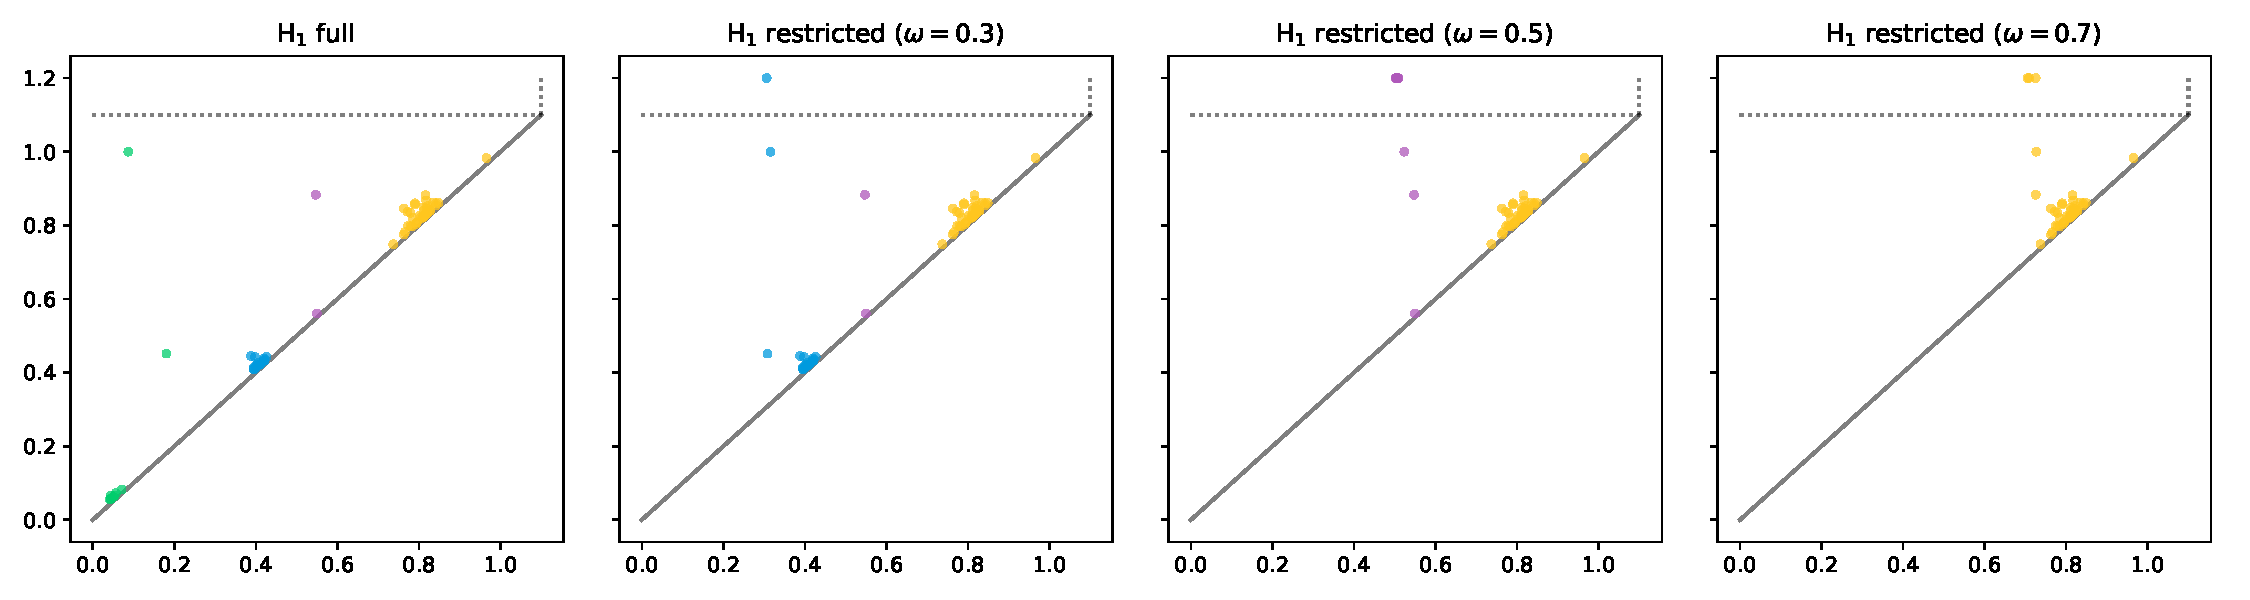
\includegraphics[trim=0 0 790 0, clip, width=0.3\textwidth]{figures/matching-full-dgm.pdf}
  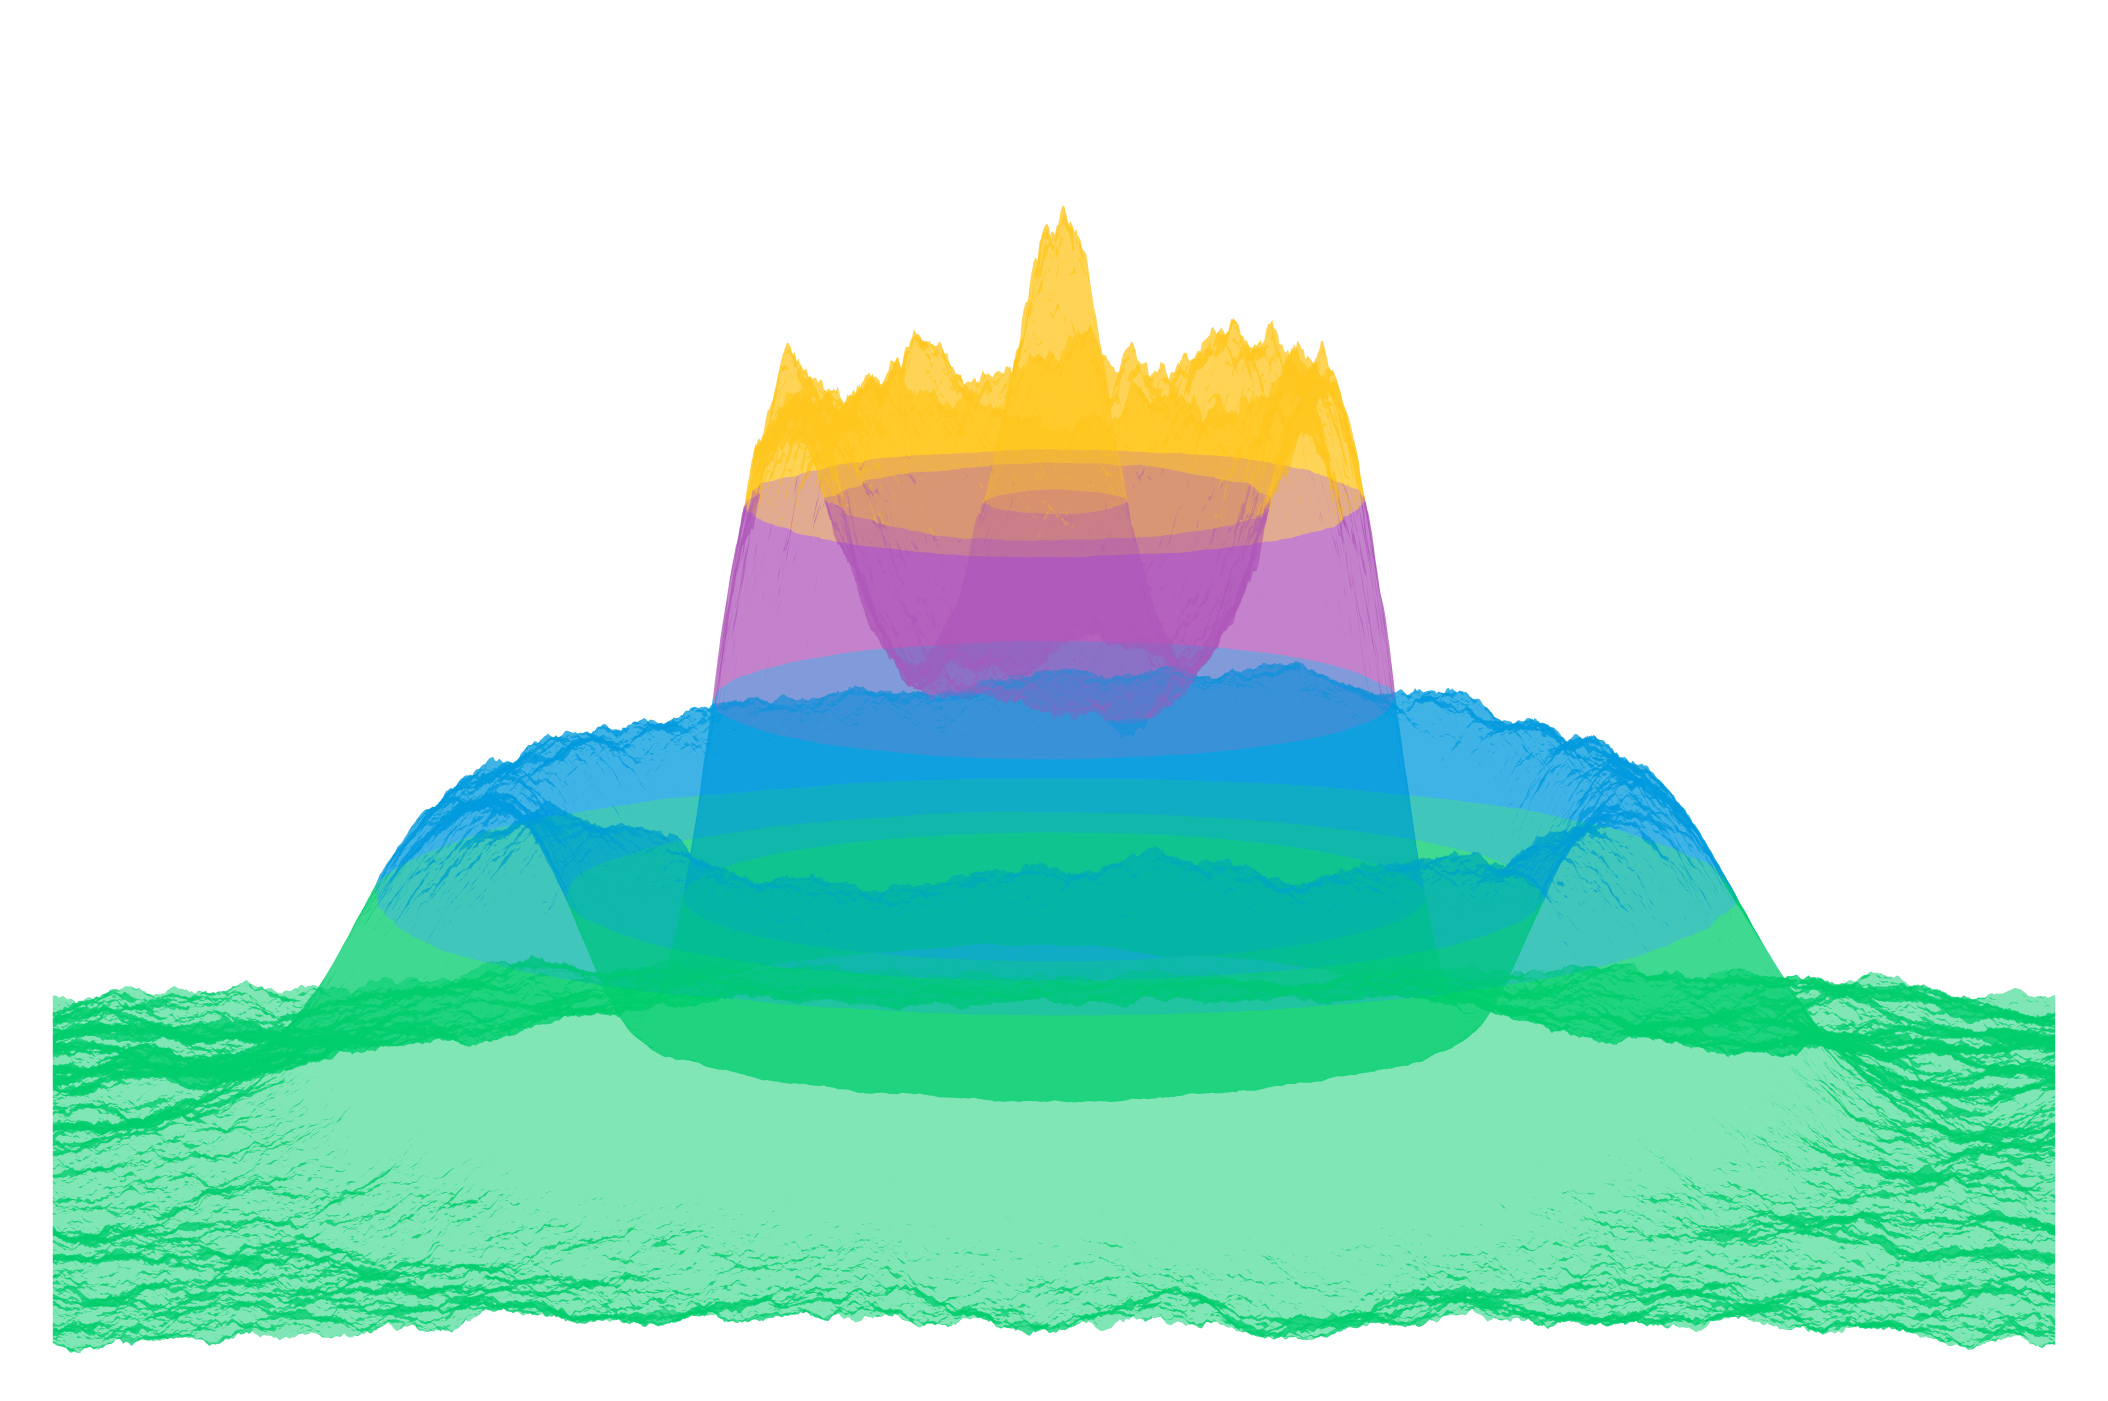
\includegraphics[trim=-350 -800 -700 -300, clip, width=0.4\textwidth]{figures/matching-full-surf_side-lowres.png}
  
\includegraphics[trim=0 -800 0 0, width=0.25\textwidth]{figures/matching-full-surf_top-lowres.png}
  % \includegraphics[trim=0 0 0 -10, clip, width=\textwidth]{scripts/figures/matching1/817_1024-3_1-1_1.png}
  \caption{The $\hom_1$ persistence diagram of the sinusoidal function pictured to the right.
  Features are colored by birth time, infinite features are drawn above the dotted line.}\label{fig:ripple1}
\end{figure}

Throughout, the four interlevel sets shown correspond to the ranges $[0, 0.3)$, $[0.3, 0.5)$, $[0.5, 0.7)$, and $[0.7, 1)$, respectively.
Our persistent homology computations were done primarily with Dionysus~\cite{morozov12dionysus} augmented with custom software for computing representative cycles of infinite features.
\footnote{3D figures were made with MayaVi, all other figures were made with Matplotlib.}
The persistent homology of our function was computed with the lower-star filtration of the Freudenthal triangulation on an $N\times N$ grid over $[-1,1]\times[-1,1]\subset\R^2$.
We take this filtration as $\{\rips^{2\delta}(P_\alpha)\}$ where $P$ is the set of grid points and $\delta = \sqrt{2} / N$.

We note that the purpose of these experiments is not to demonstrate the effectiveness of our approximation by Rips complexes, but to demonstrate the relationships between restricted, relative, and truncated diagrams.
Therefore, for simplicity, we will omit the inclusion $\rips^{2\delta}(P_\alpha)\hookrightarrow\rips^{4\delta}(P_\alpha)$ and take the persistent homology of $\{\rips^{2\delta}(P_\alpha)\}$ with sufficiently small $\delta$ as our ground-truth.
However, in order to keep our diagrams clean we show only those features a distance at least $4\delta$ from the diagonal.
Note that these features are \emph{not} removed from the diagram, and considered in all computations.

In the following we will take $N = 1024$, so $\delta\approx 1.4\times 10^{-3}$, as our ground-truth.
Figure~\ref{fig:ripple1} shows the \emph{full diagram} of our function with features colored by birth time.
Therefore, for $\omega = 0.3, 0.5, 0.7$ the \emph{truncated diagram} is obtained by successively removing features in each interlevel set.
Recall the \emph{restricted diagram} is that of the function restricted to the $\omega$ \emph{superlvel} set filtration, and computed with $\{\rips^{2\delta}(P_\alpha\setminus Q_\omega)\}$.
We will compare this restricted diagram with the \emph{relative diagram}, computed as the relative persistent homology of the filtration of pairs $\{\rips^{2\delta}(P_\alpha, Q_\omega)\}$.

\paragraph*{The issue with restricted diagrams.}

In order to get an initial sense of the difference between relative and restricted diagrams we first compare the bottleneck distance of each to the truncated diagram.
As we have shown the relative diagram is equal to the truncated diagram with additional infinite features we will remove all infinite features from the bottleneck computation.
We therefore expect the distance between the relative and truncated diagrams to be zero for $N=1024$.

Figure~\ref{fig:bottleneck} shows the bottleneck distance from the truncated diagram at full resolution ($N = 1024$) to both the relative and restricted diagrams with varying resolution.
Specifically, the function on a $1024\times 1024$ grid is down-sampled to grids ranging from $64\times 64$ to $1024\times 1024$.
We also show the expected bottleneck distance to the true truncated diagram given by the interleaving in Theorem~\ref{thm:interleaving_main_2} in black.

\begin{figure}[htbp]
  \centering
  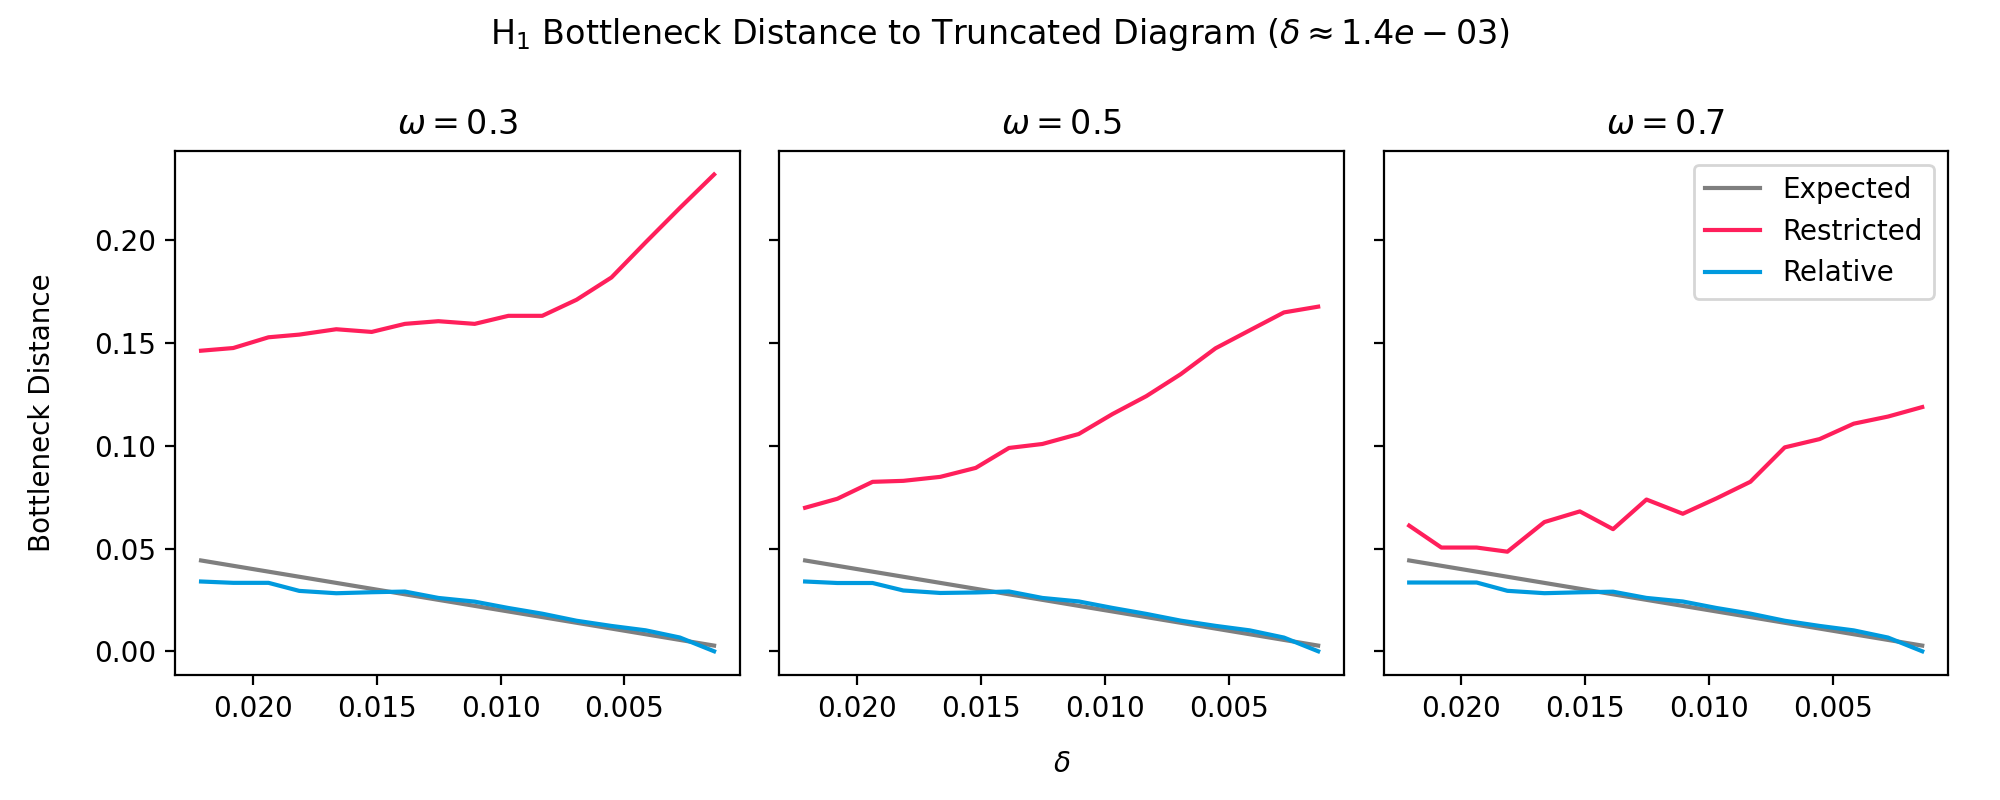
\includegraphics[width=0.95\textwidth]{figures/matching-bottleneck_delta.png}
  \caption{Comparison of the bottleneck distance between the truncated diagram and those of the restricted and relative diagrams with increasing resolution.}\label{fig:bottleneck}
\end{figure}

As we can see, the relative diagram performs better than the restricted diagram, which diverges with increasing resolution.
The reason for this is shown in Figure~\ref{fig:restricted} which depicts the restricted diagrams at $\omega = 0.3, 0.5,$ and $0.7$ at full resolution.
Recall that 1-dimensional features that are born before $\omega$ and die after $\omega$ become infinite 2-dimensional features in the relative diagram, with birth time equal to the death time of the corresponding feature in the full diagram.
These same features remain 1-dimensional figures in the restricted diagram, but with their birth times shifted to $\omega$.
Indeed, the resulting restricted diagram may be closer to the full diagram for sufficiently small $\omega$.
However, the distance will be proportional to the difference between $\omega$ and the true birth time.

\begin{figure}[htbp]
  \centering
  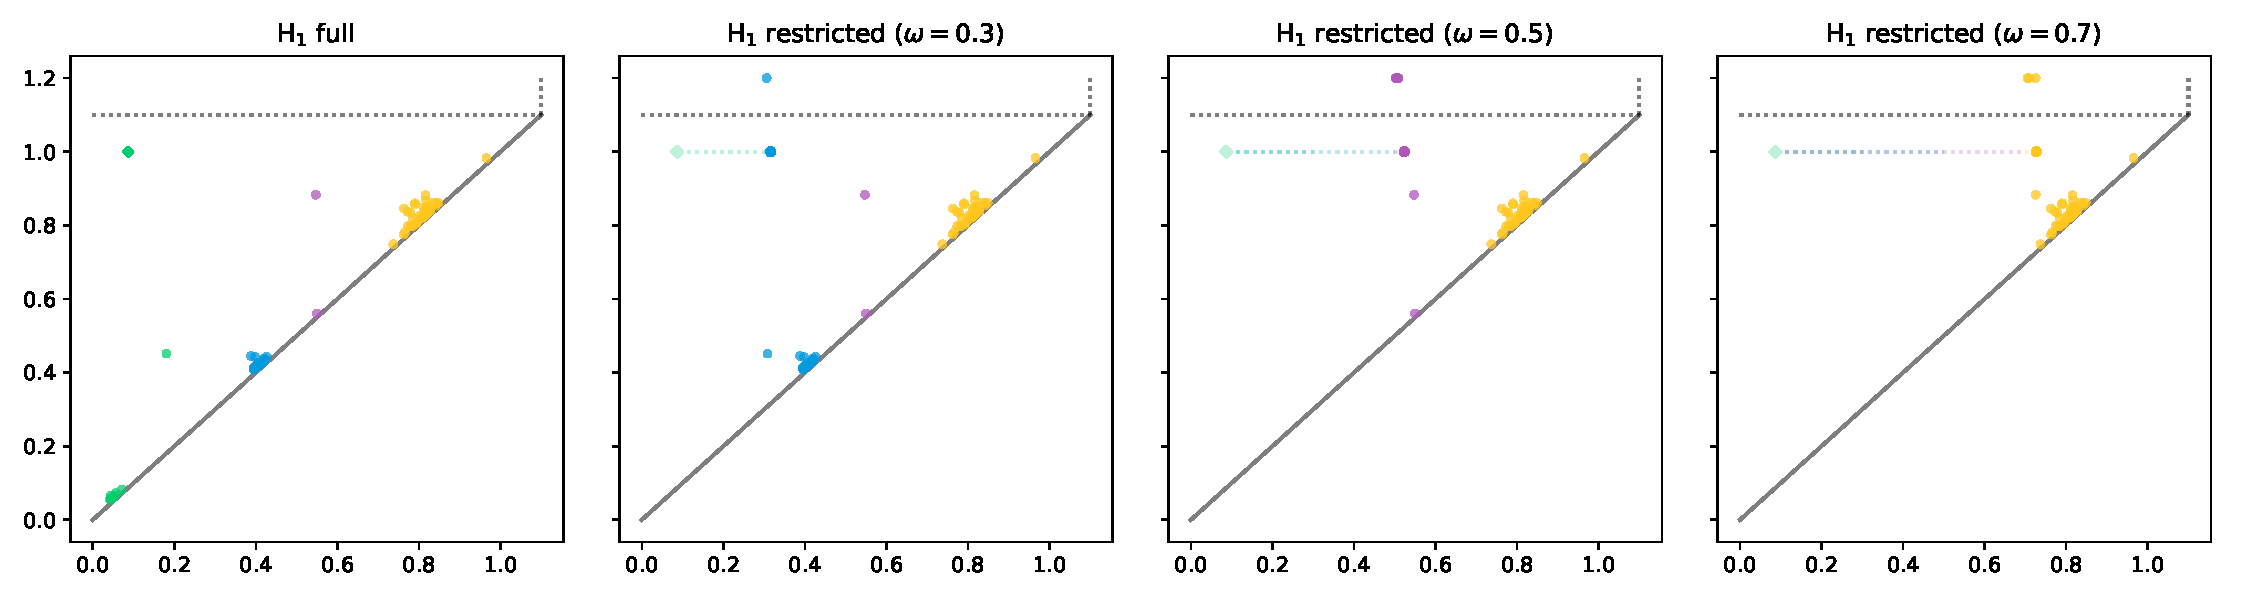
\includegraphics[trim=0 0 -10 0, clip, width=\textwidth]{figures/matching-dgm-1.pdf}
  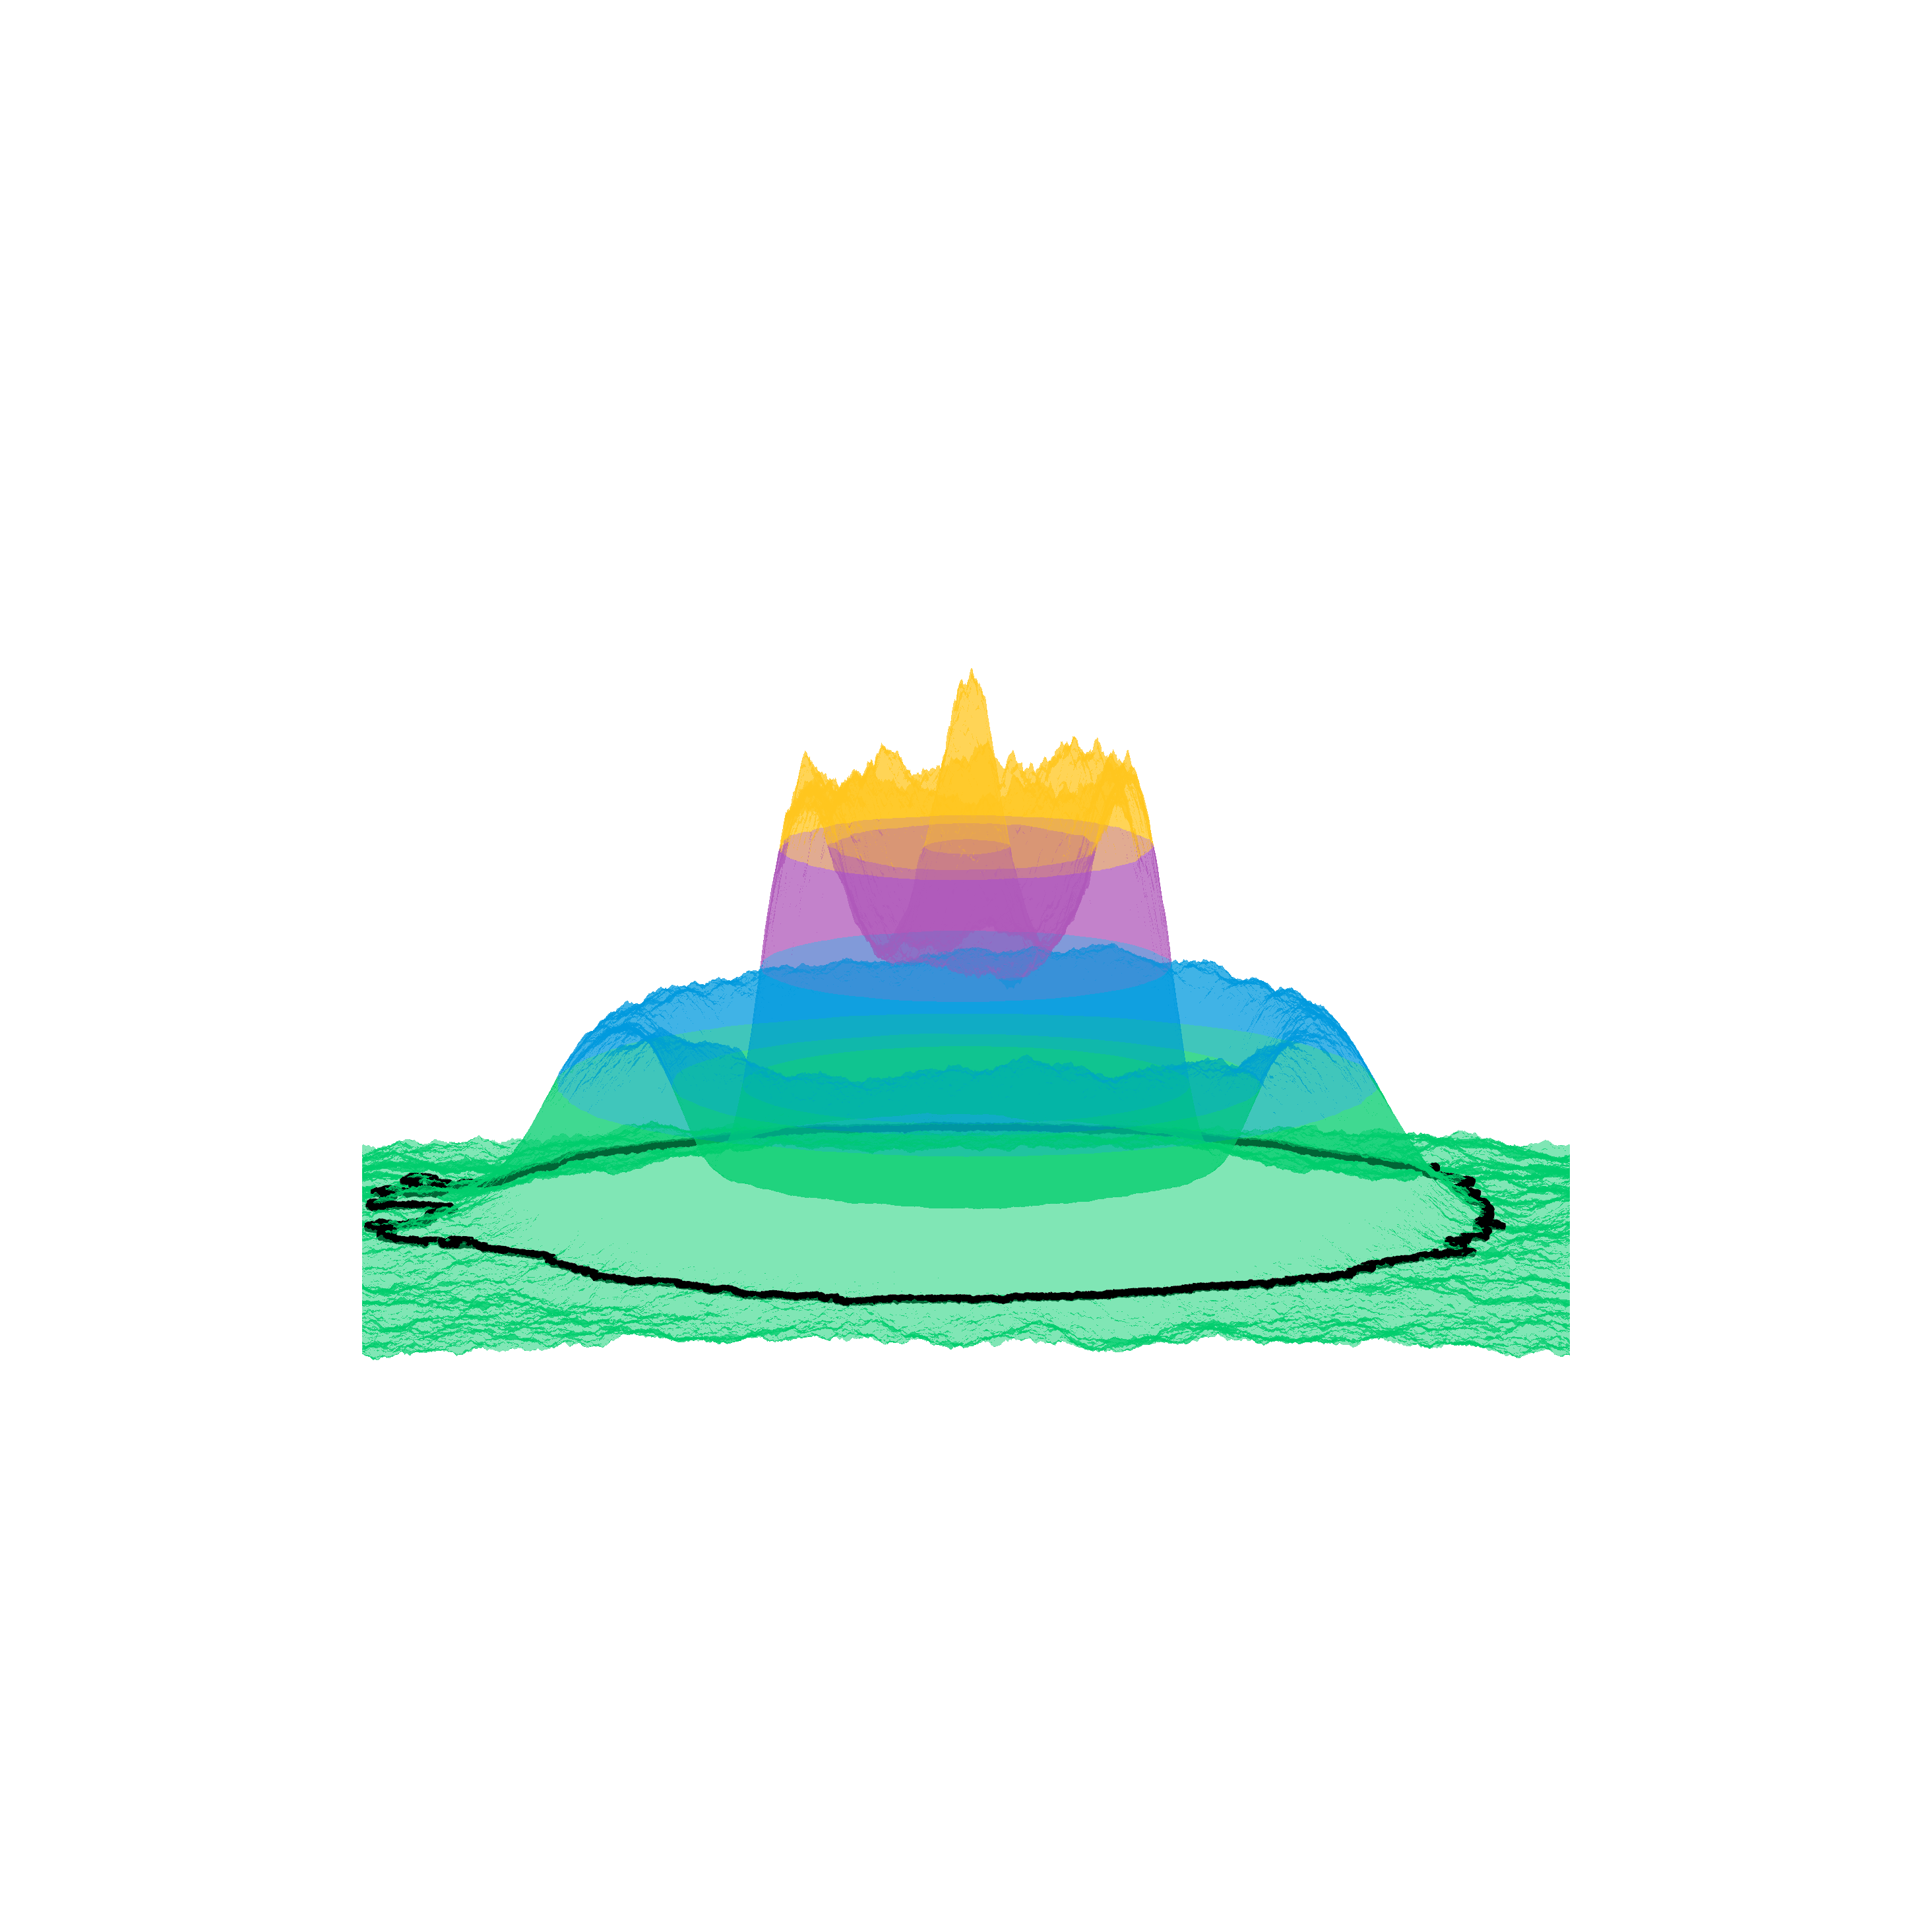
\includegraphics[trim=500 800 500 800, clip, width=0.24\textwidth]{figures/matching-surf_side-1.png}
  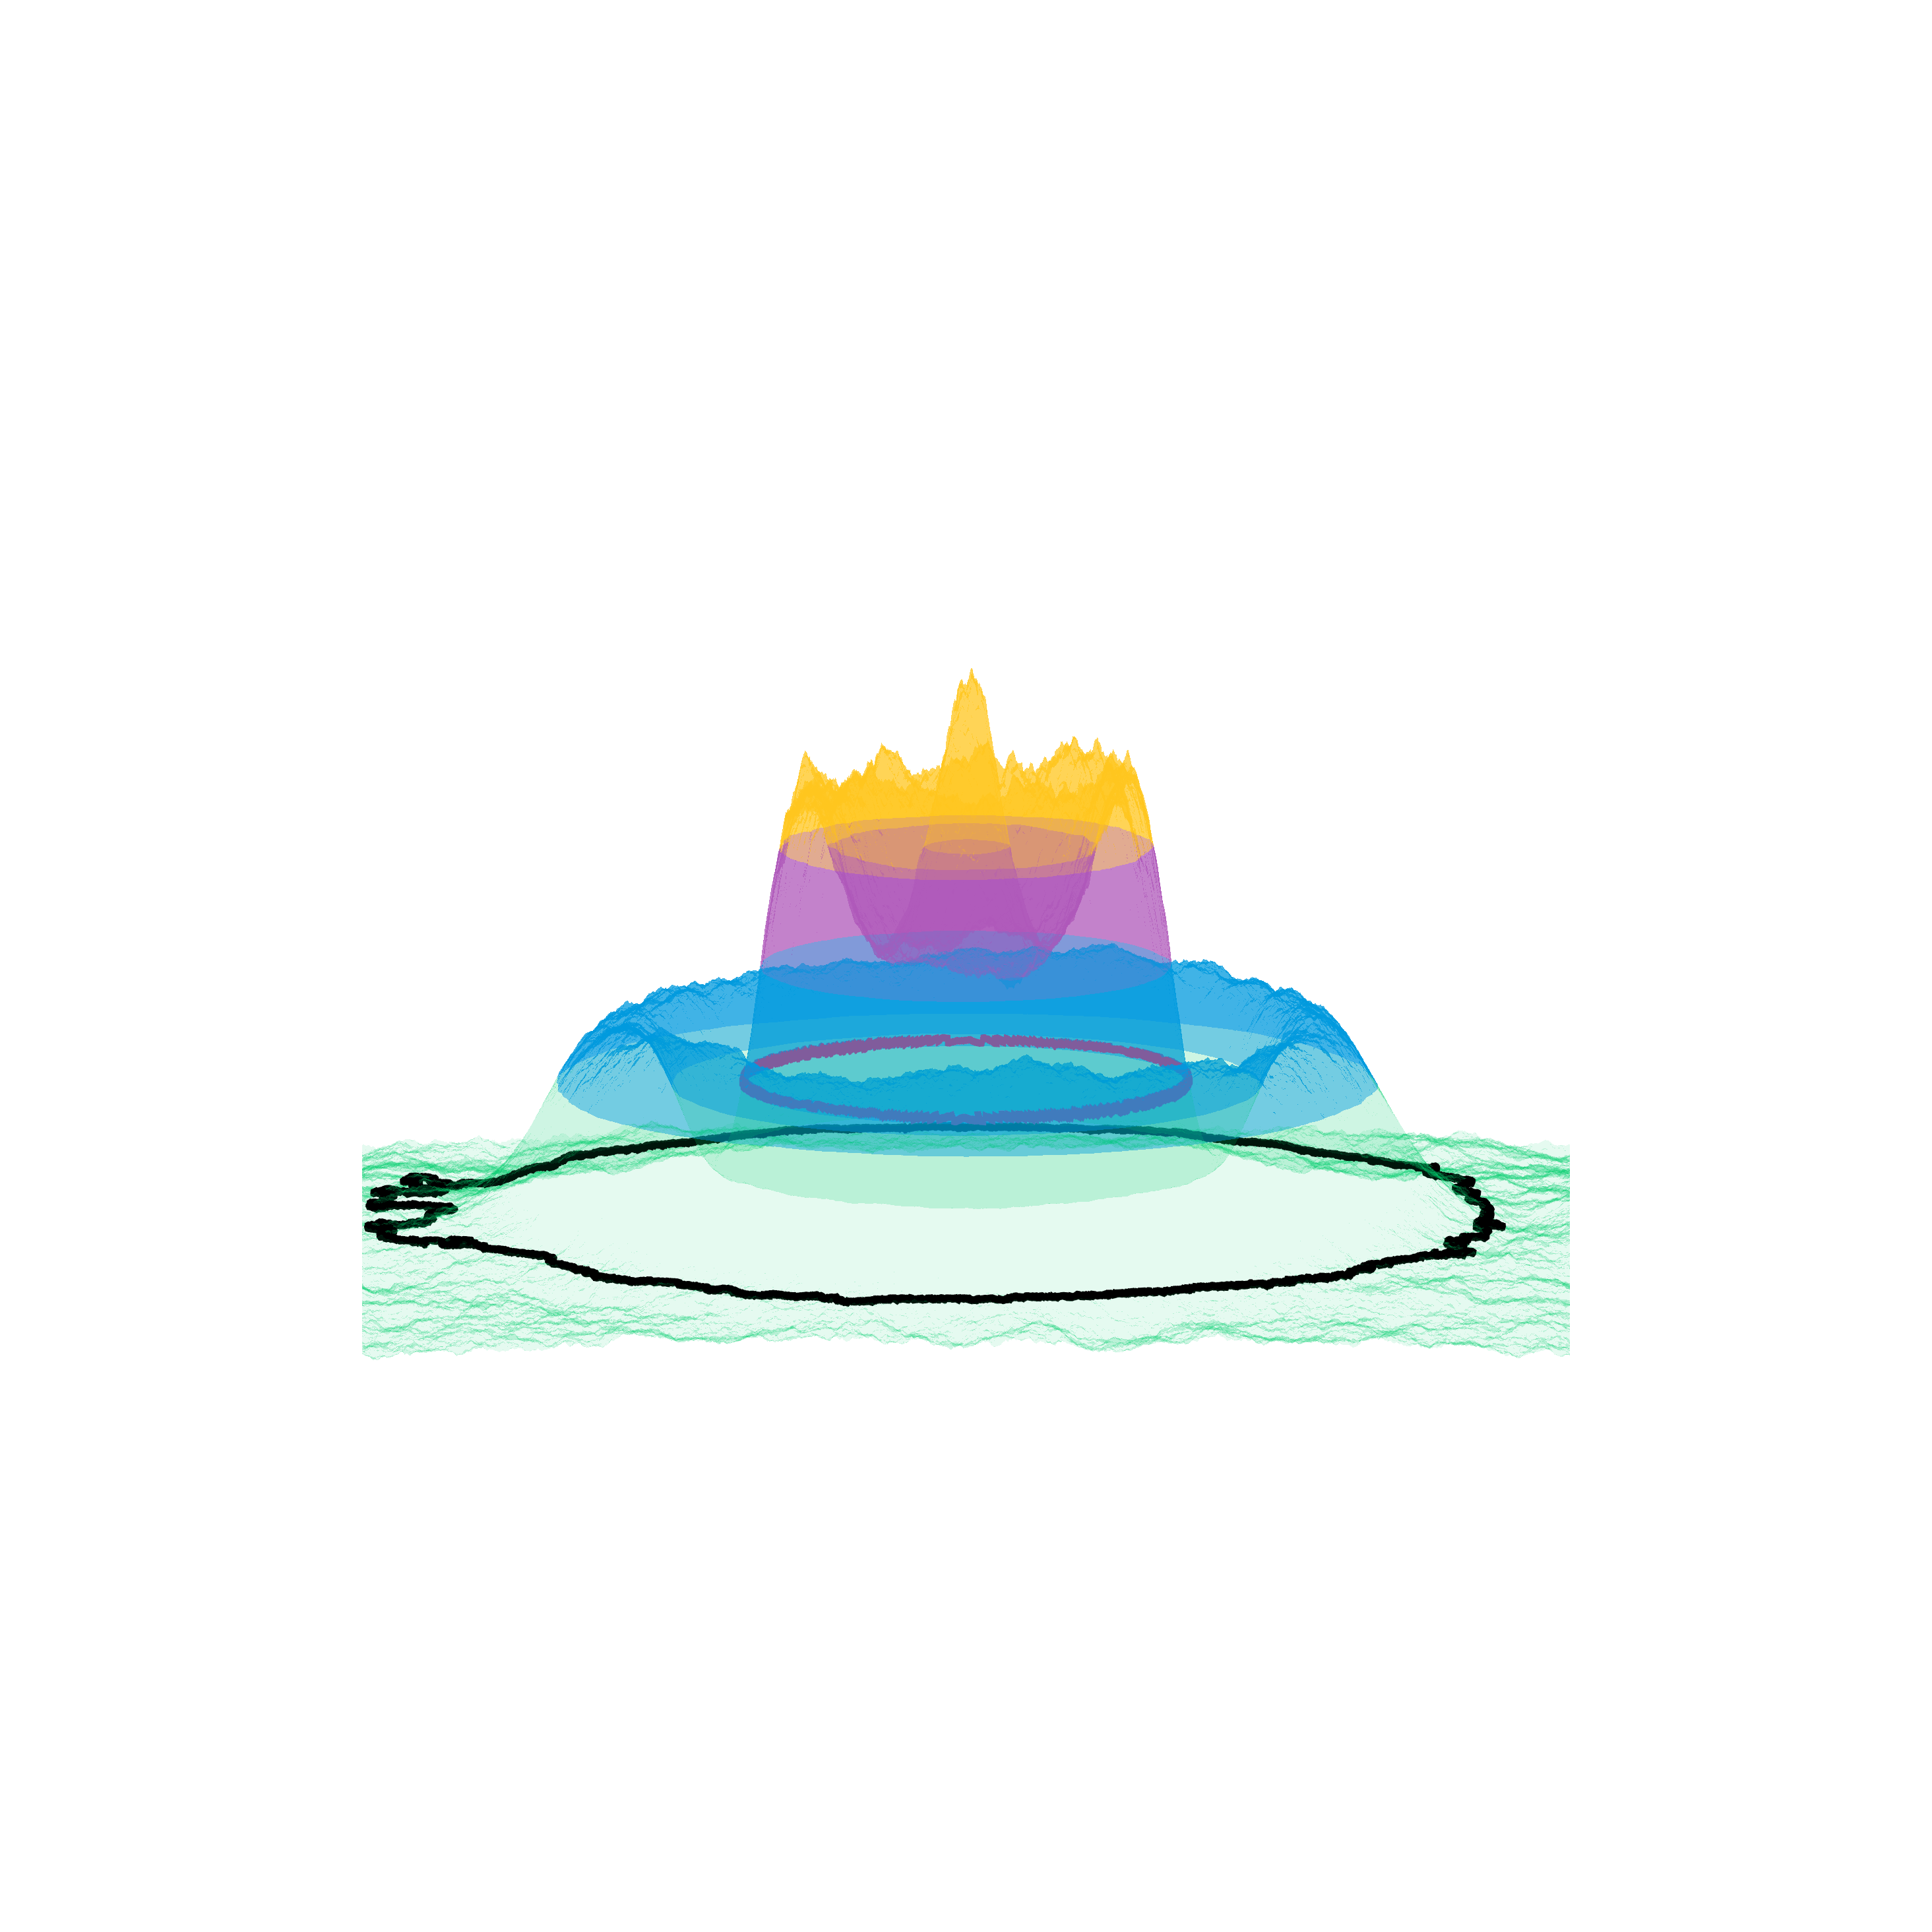
\includegraphics[trim=500 800 500 800, clip, width=0.24\textwidth]{figures/matching-surf_side-1_0.png}
  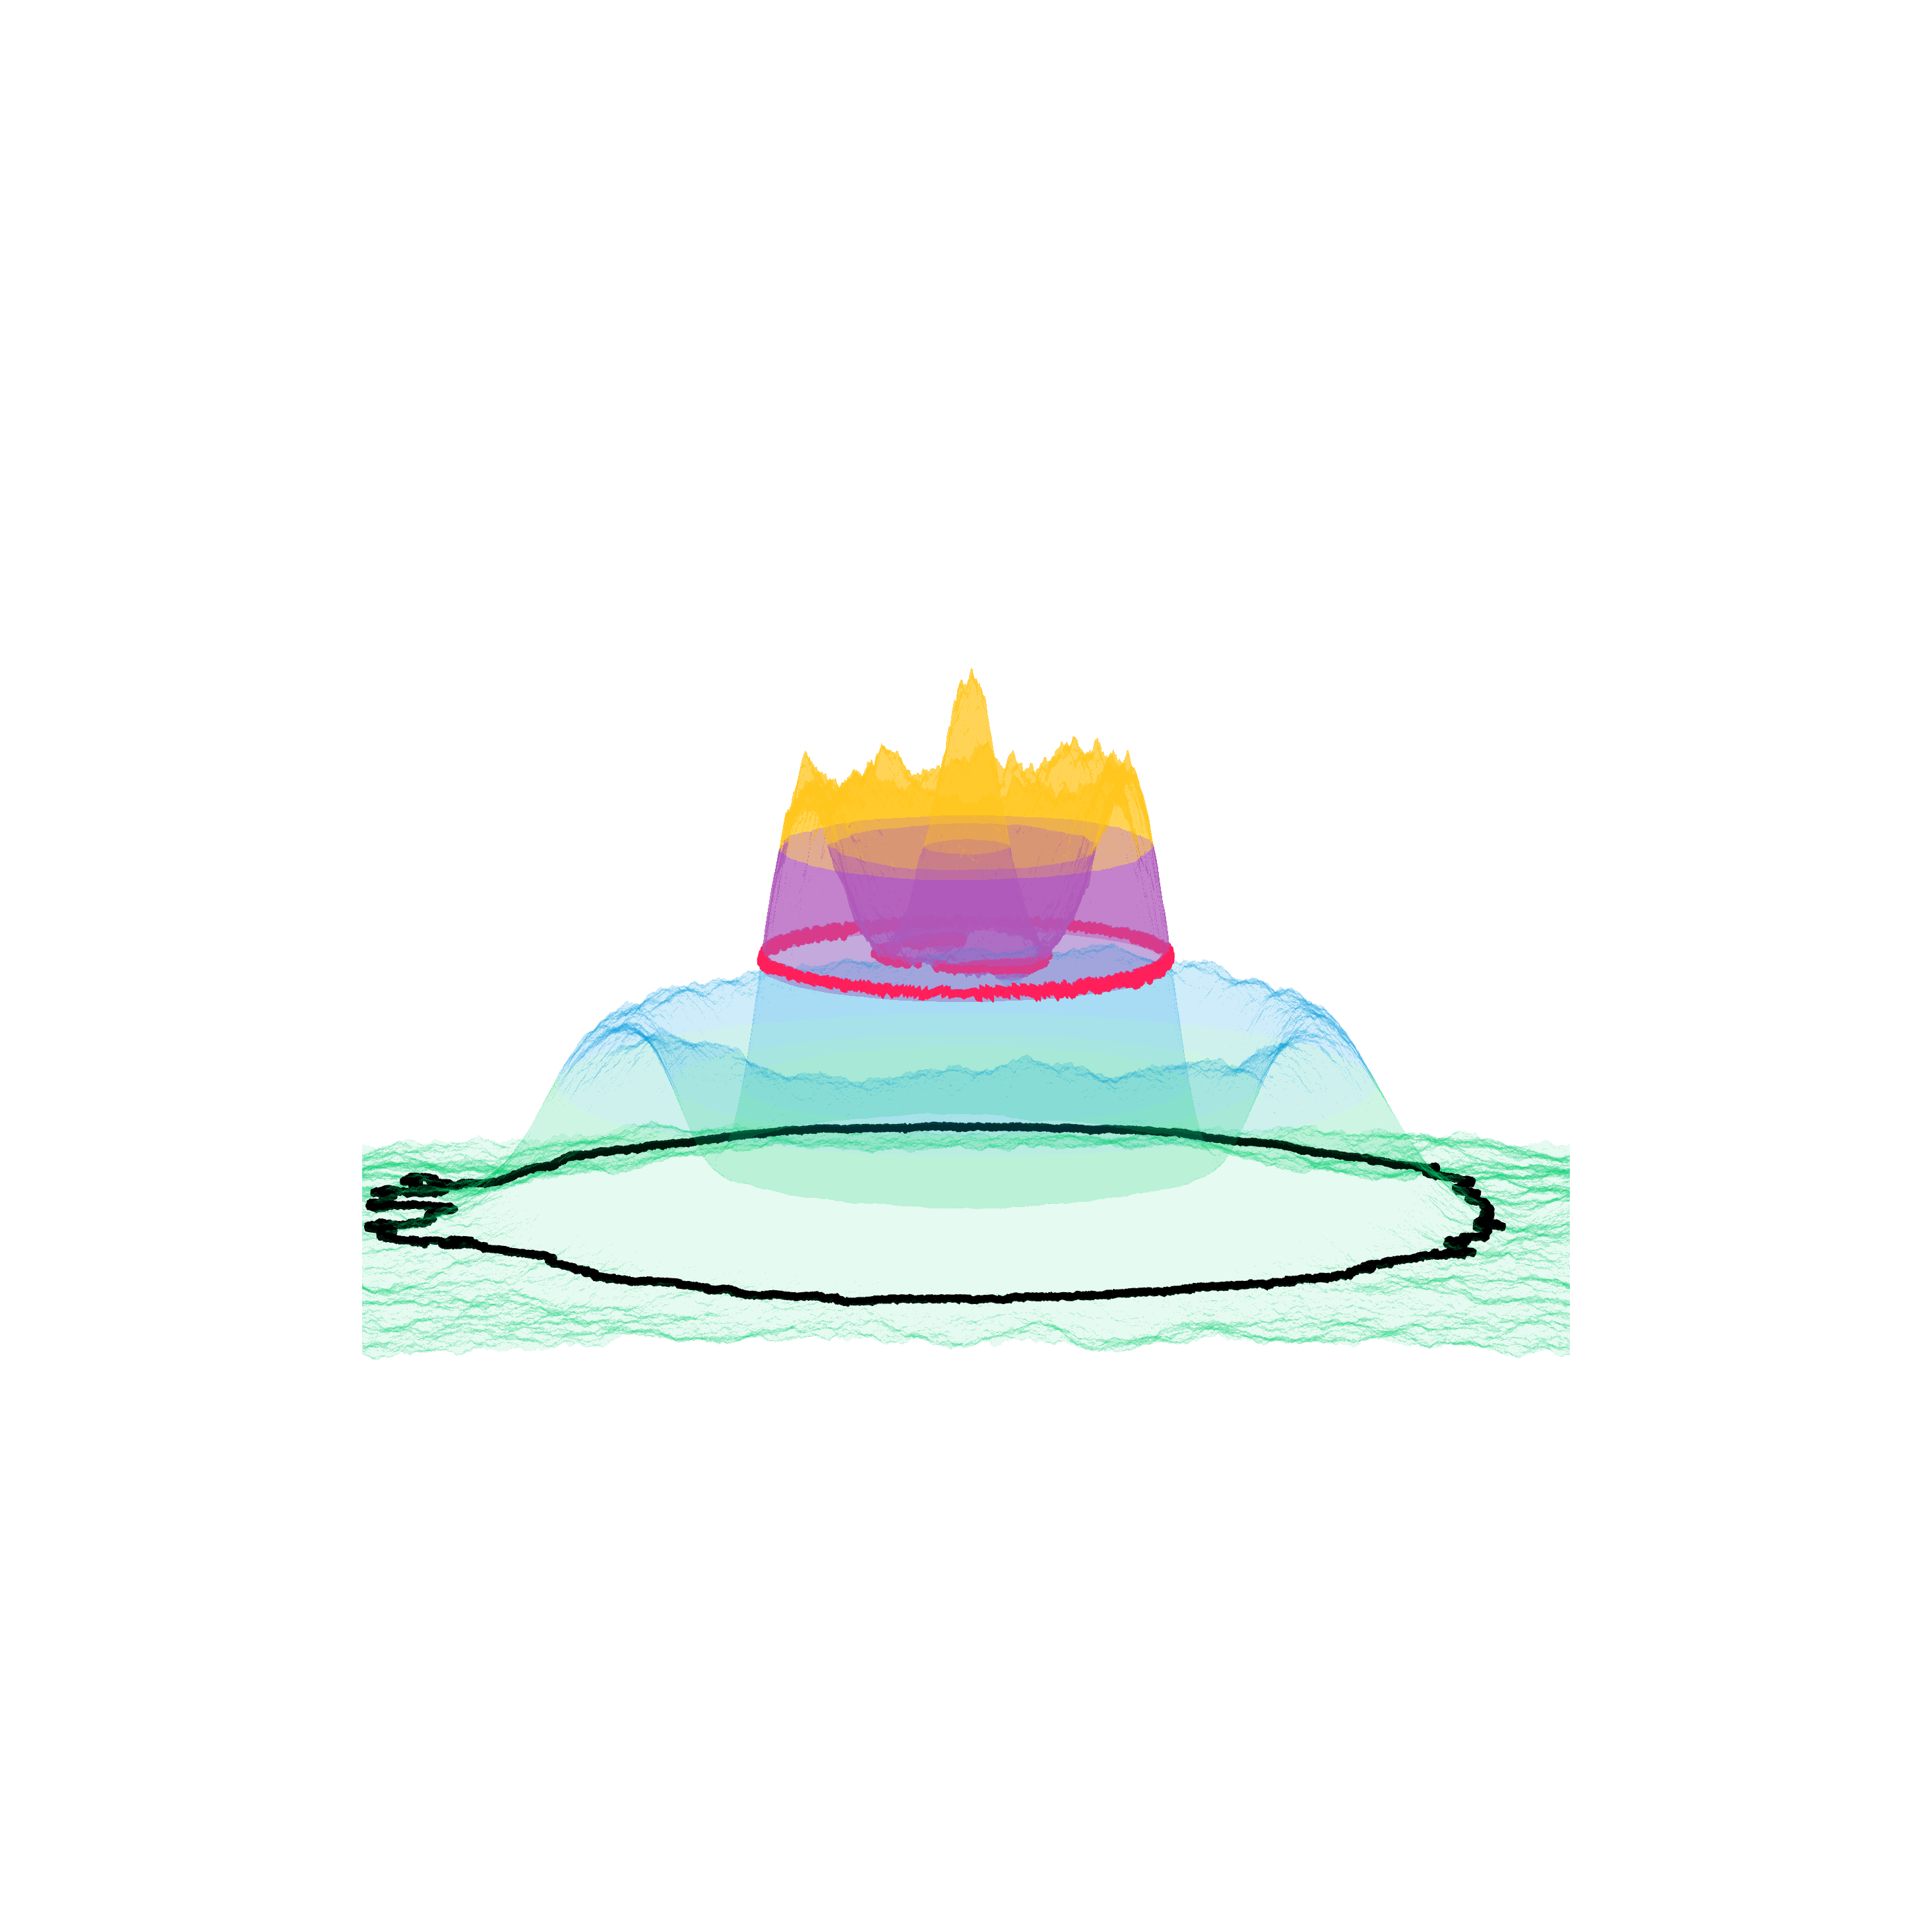
\includegraphics[trim=500 800 500 800, clip, width=0.24\textwidth]{figures/matching-surf_side-1_1.png}
  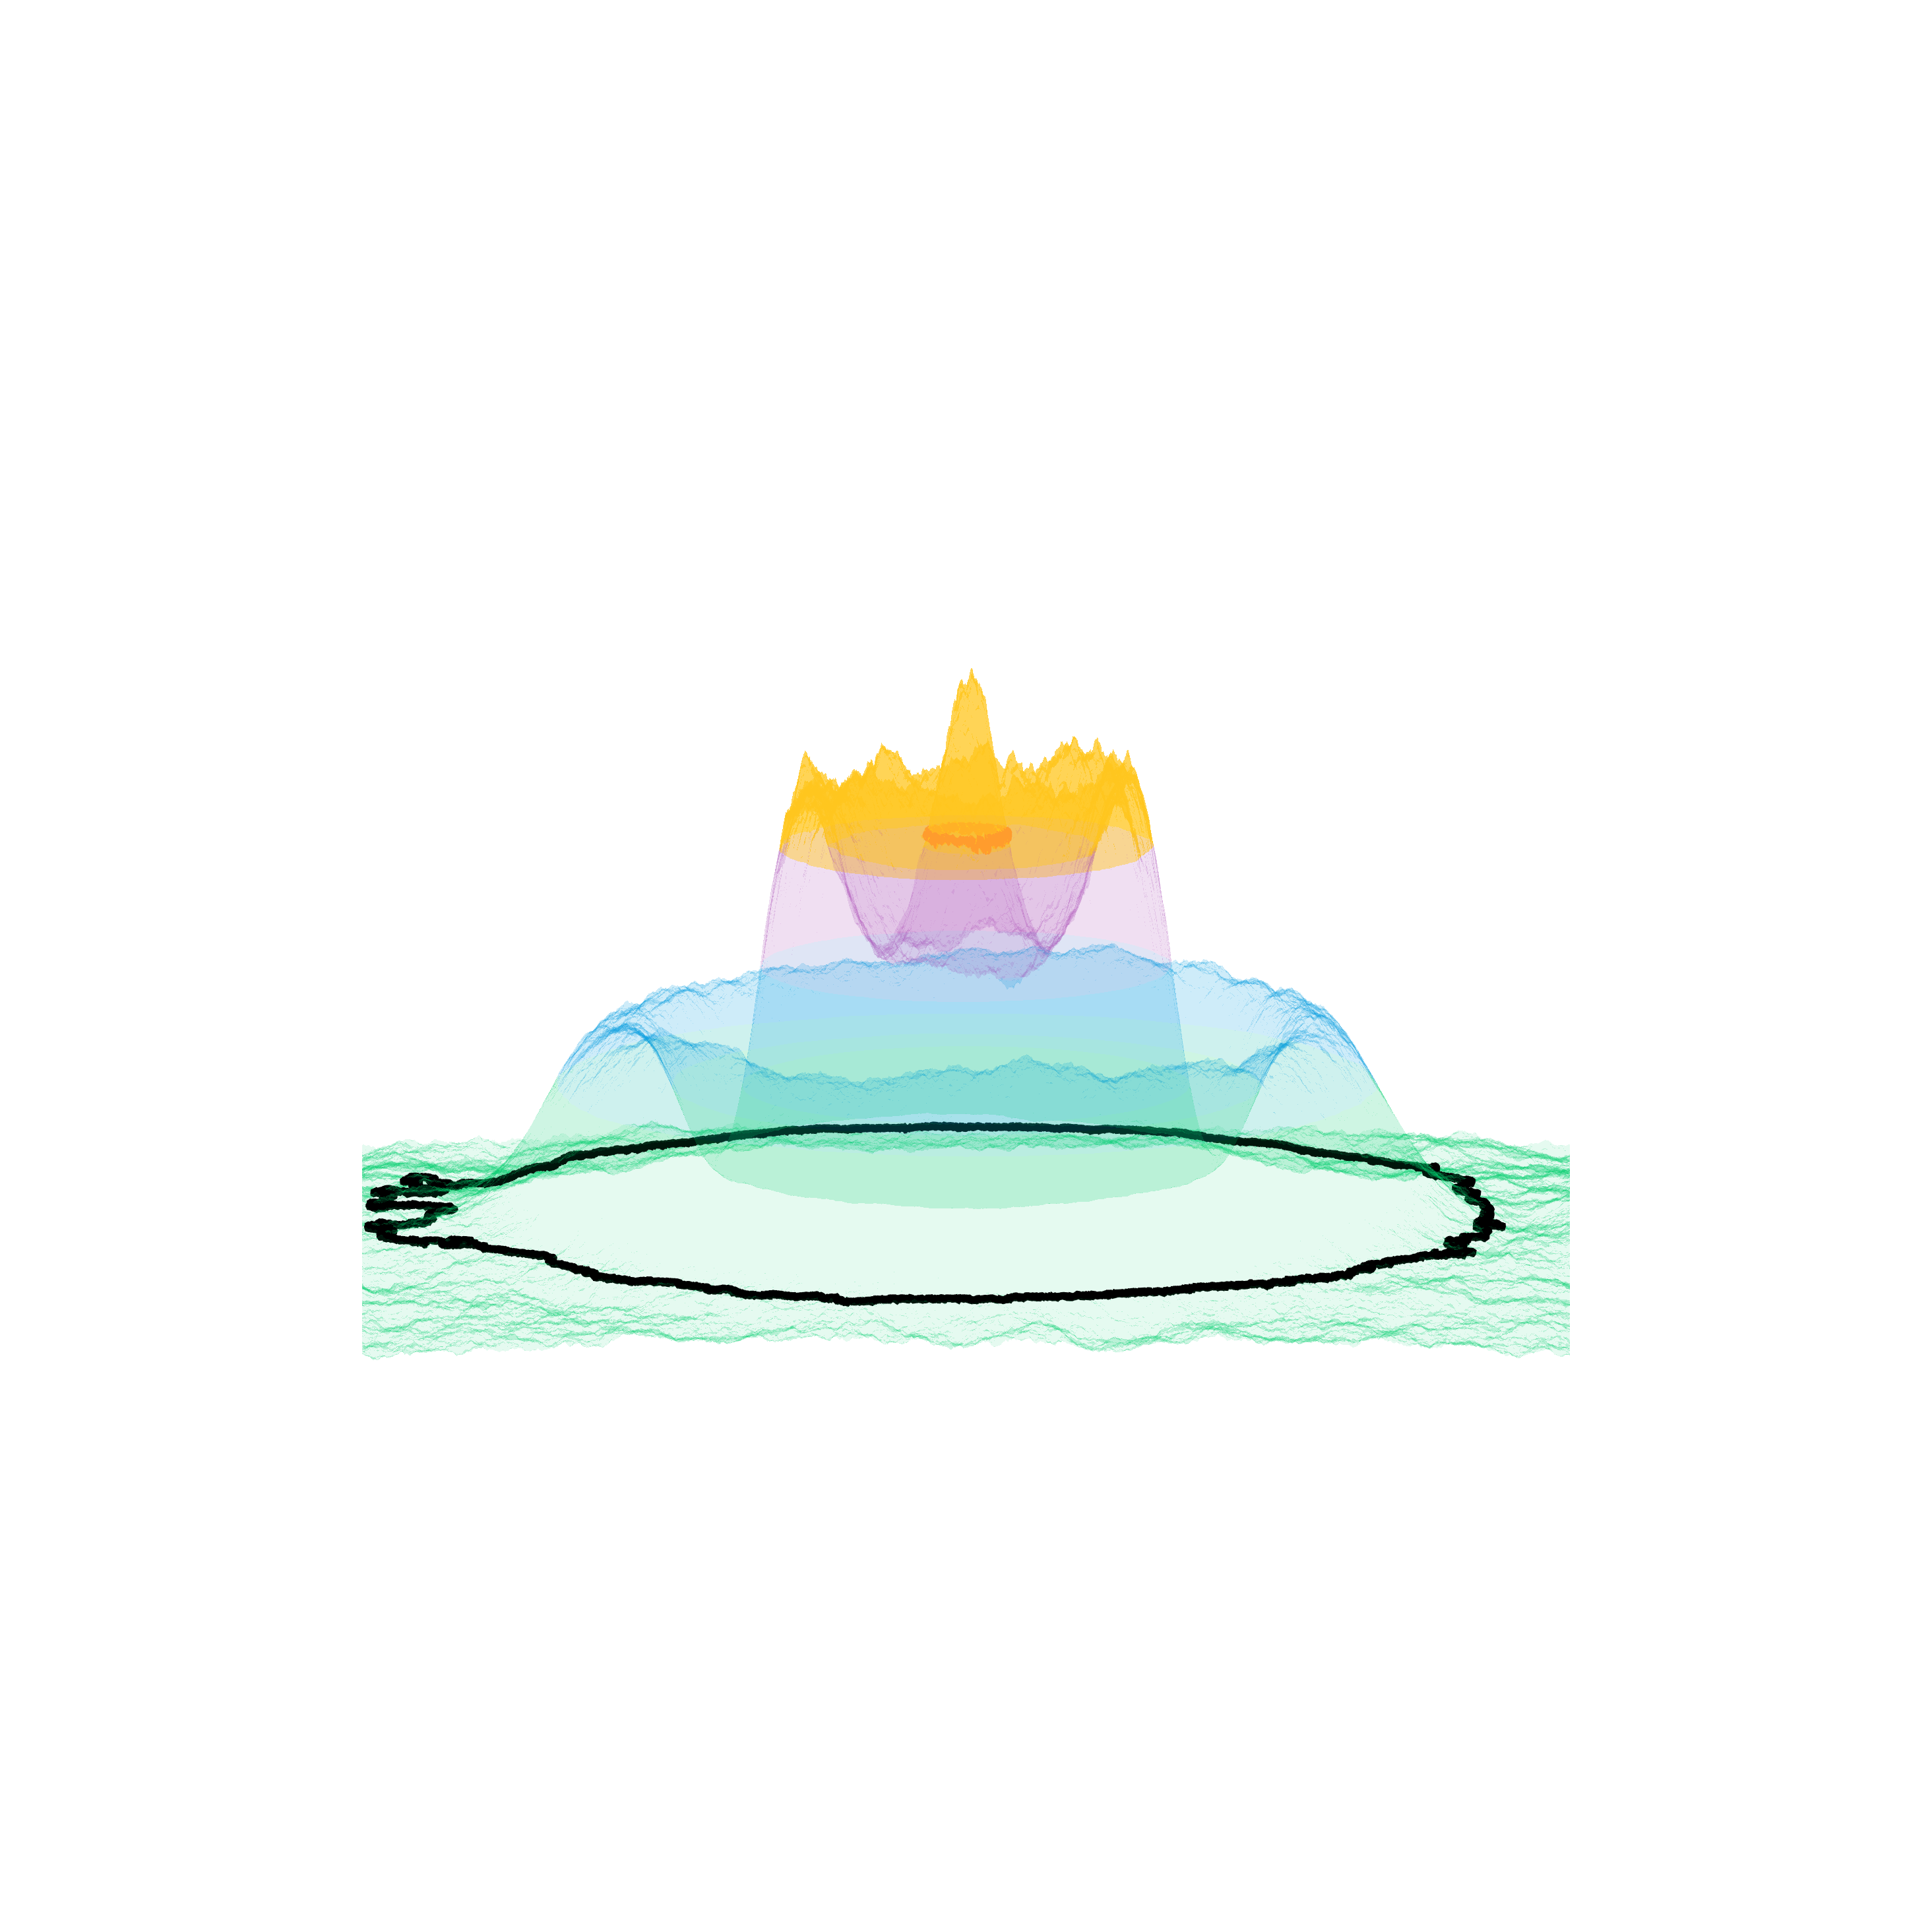
\includegraphics[trim=500 800 500 800, clip, width=0.24\textwidth]{figures/matching-surf_side-1_2.png}
  
\includegraphics[trim=500 500 500 500, clip, width=0.24\textwidth]{figures/matching-surf_top-1.png}
  
\includegraphics[trim=500 500 500 500, clip, width=0.24\textwidth]{figures/matching-surf_top-1_0.png}
  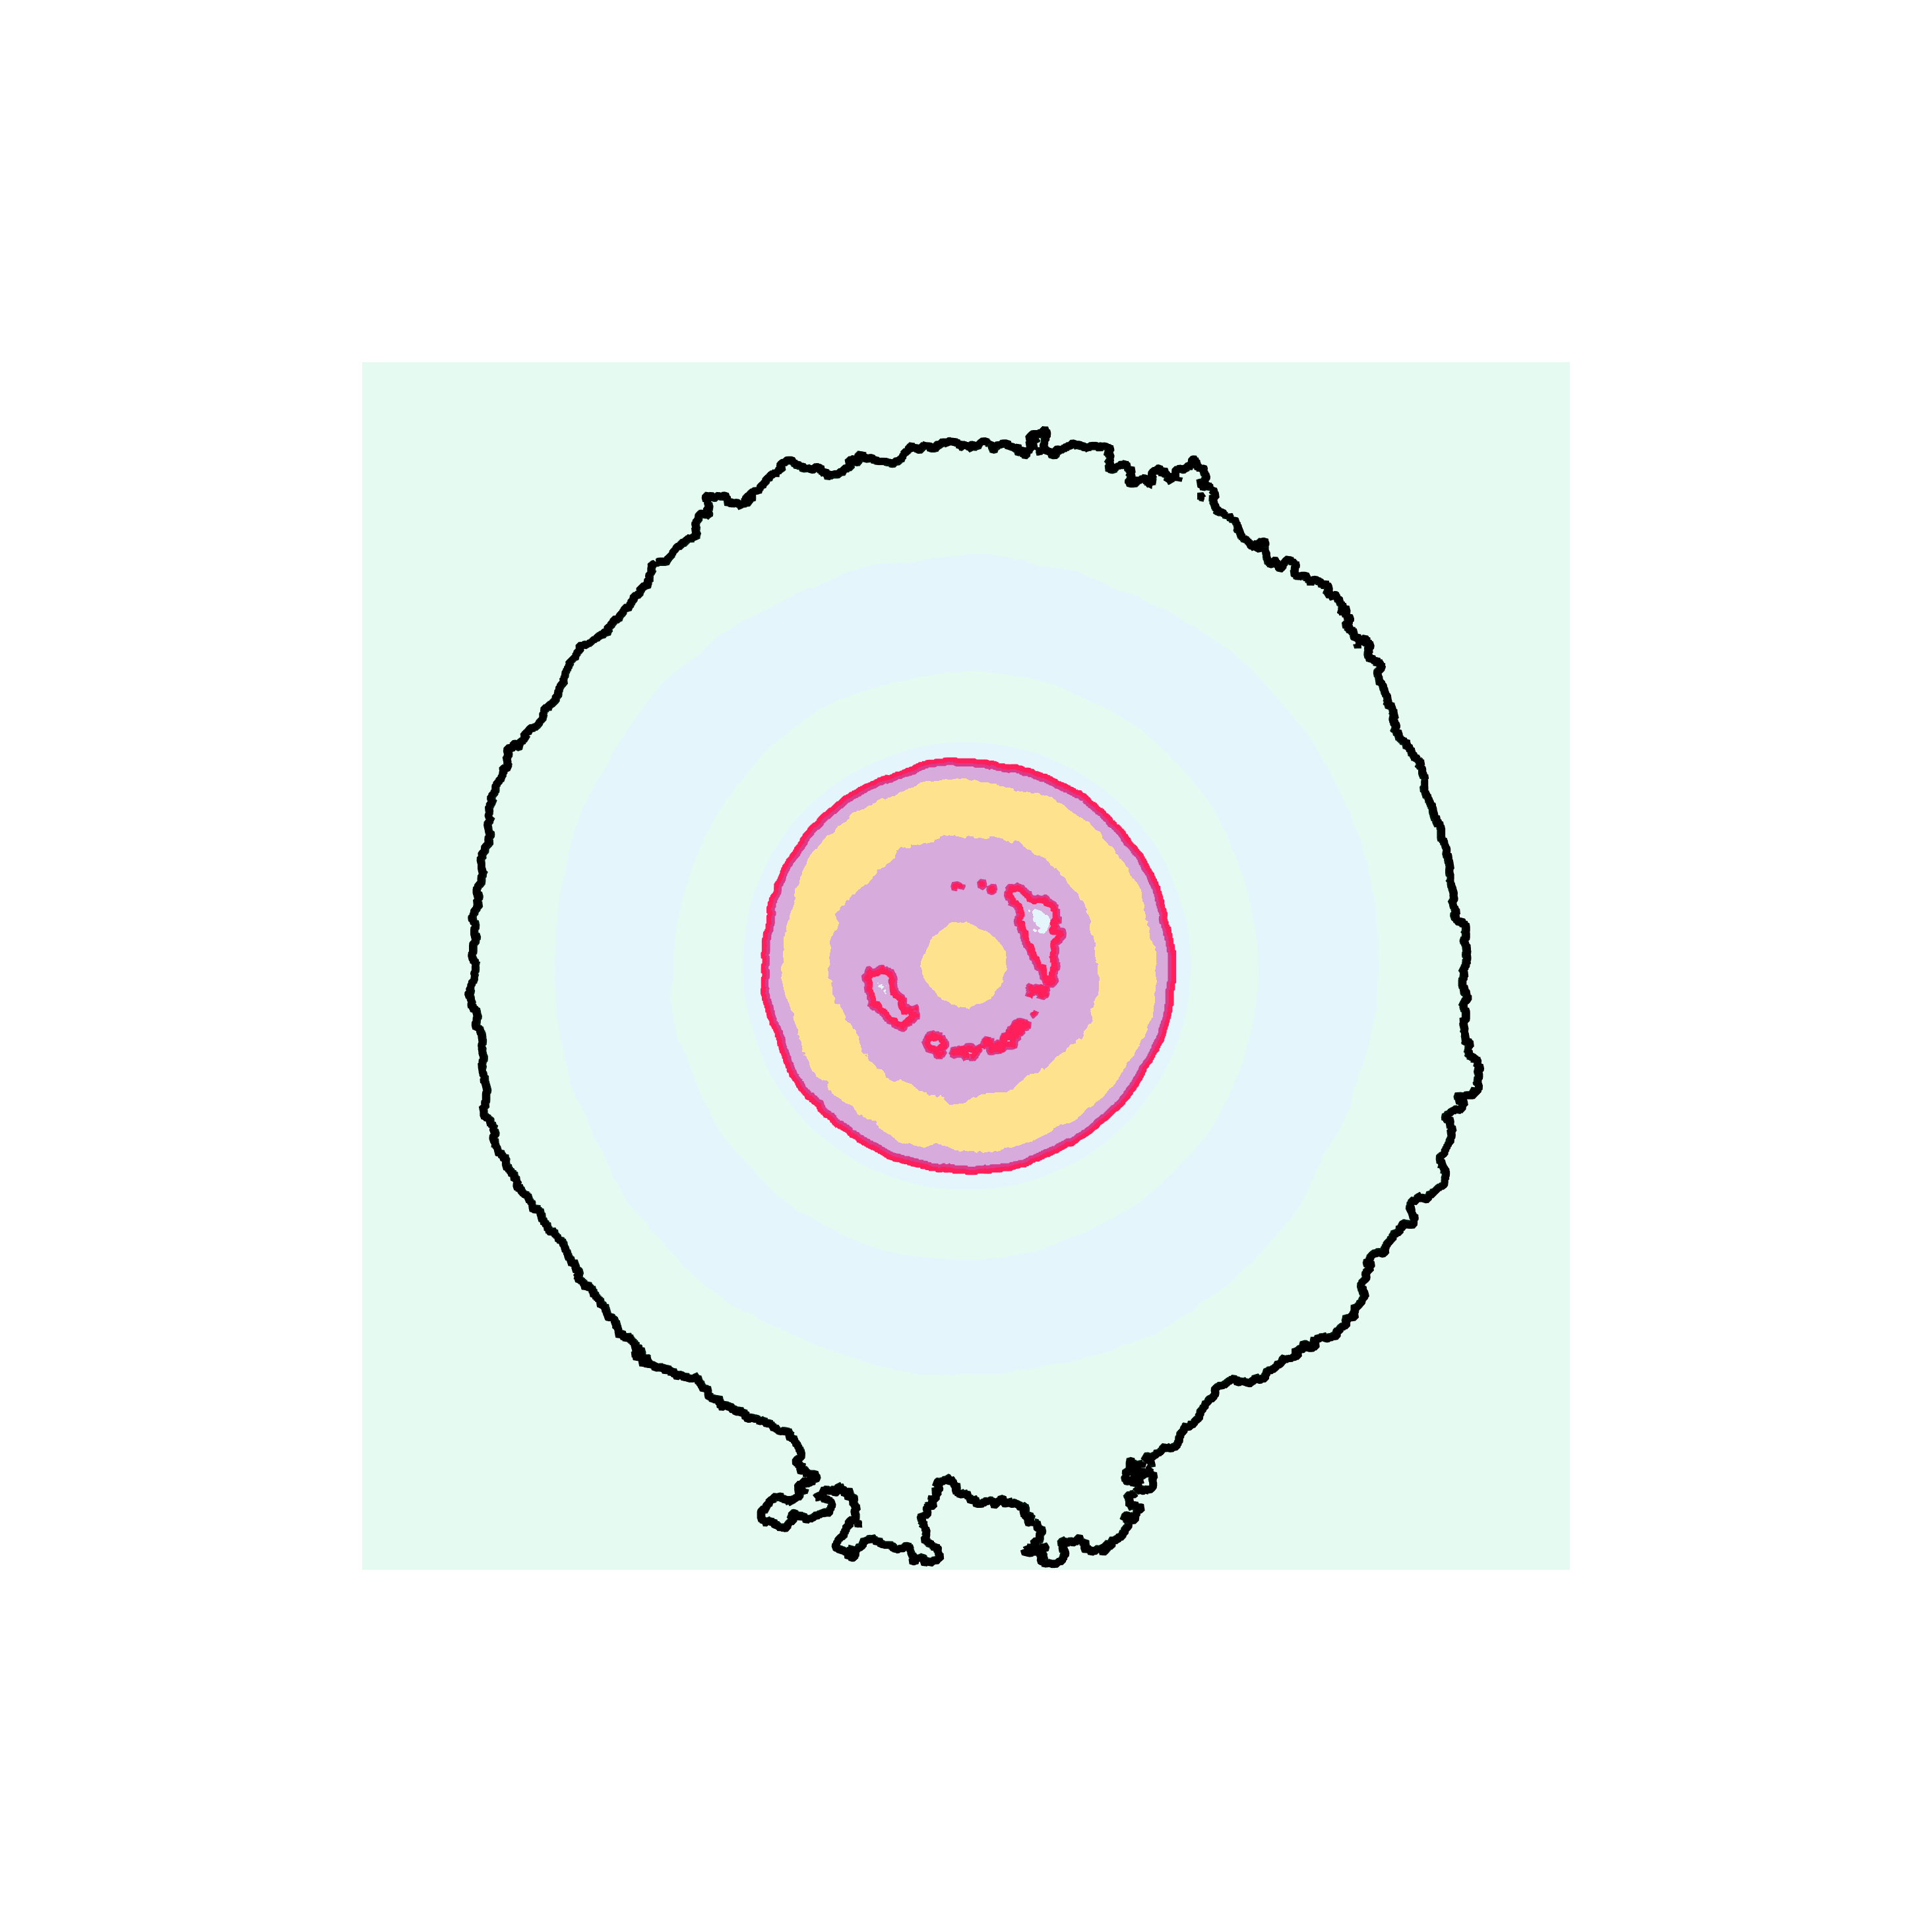
\includegraphics[trim=500 500 500 500, clip, width=0.24\textwidth]{figures/matching-surf_top-1_1.png}
  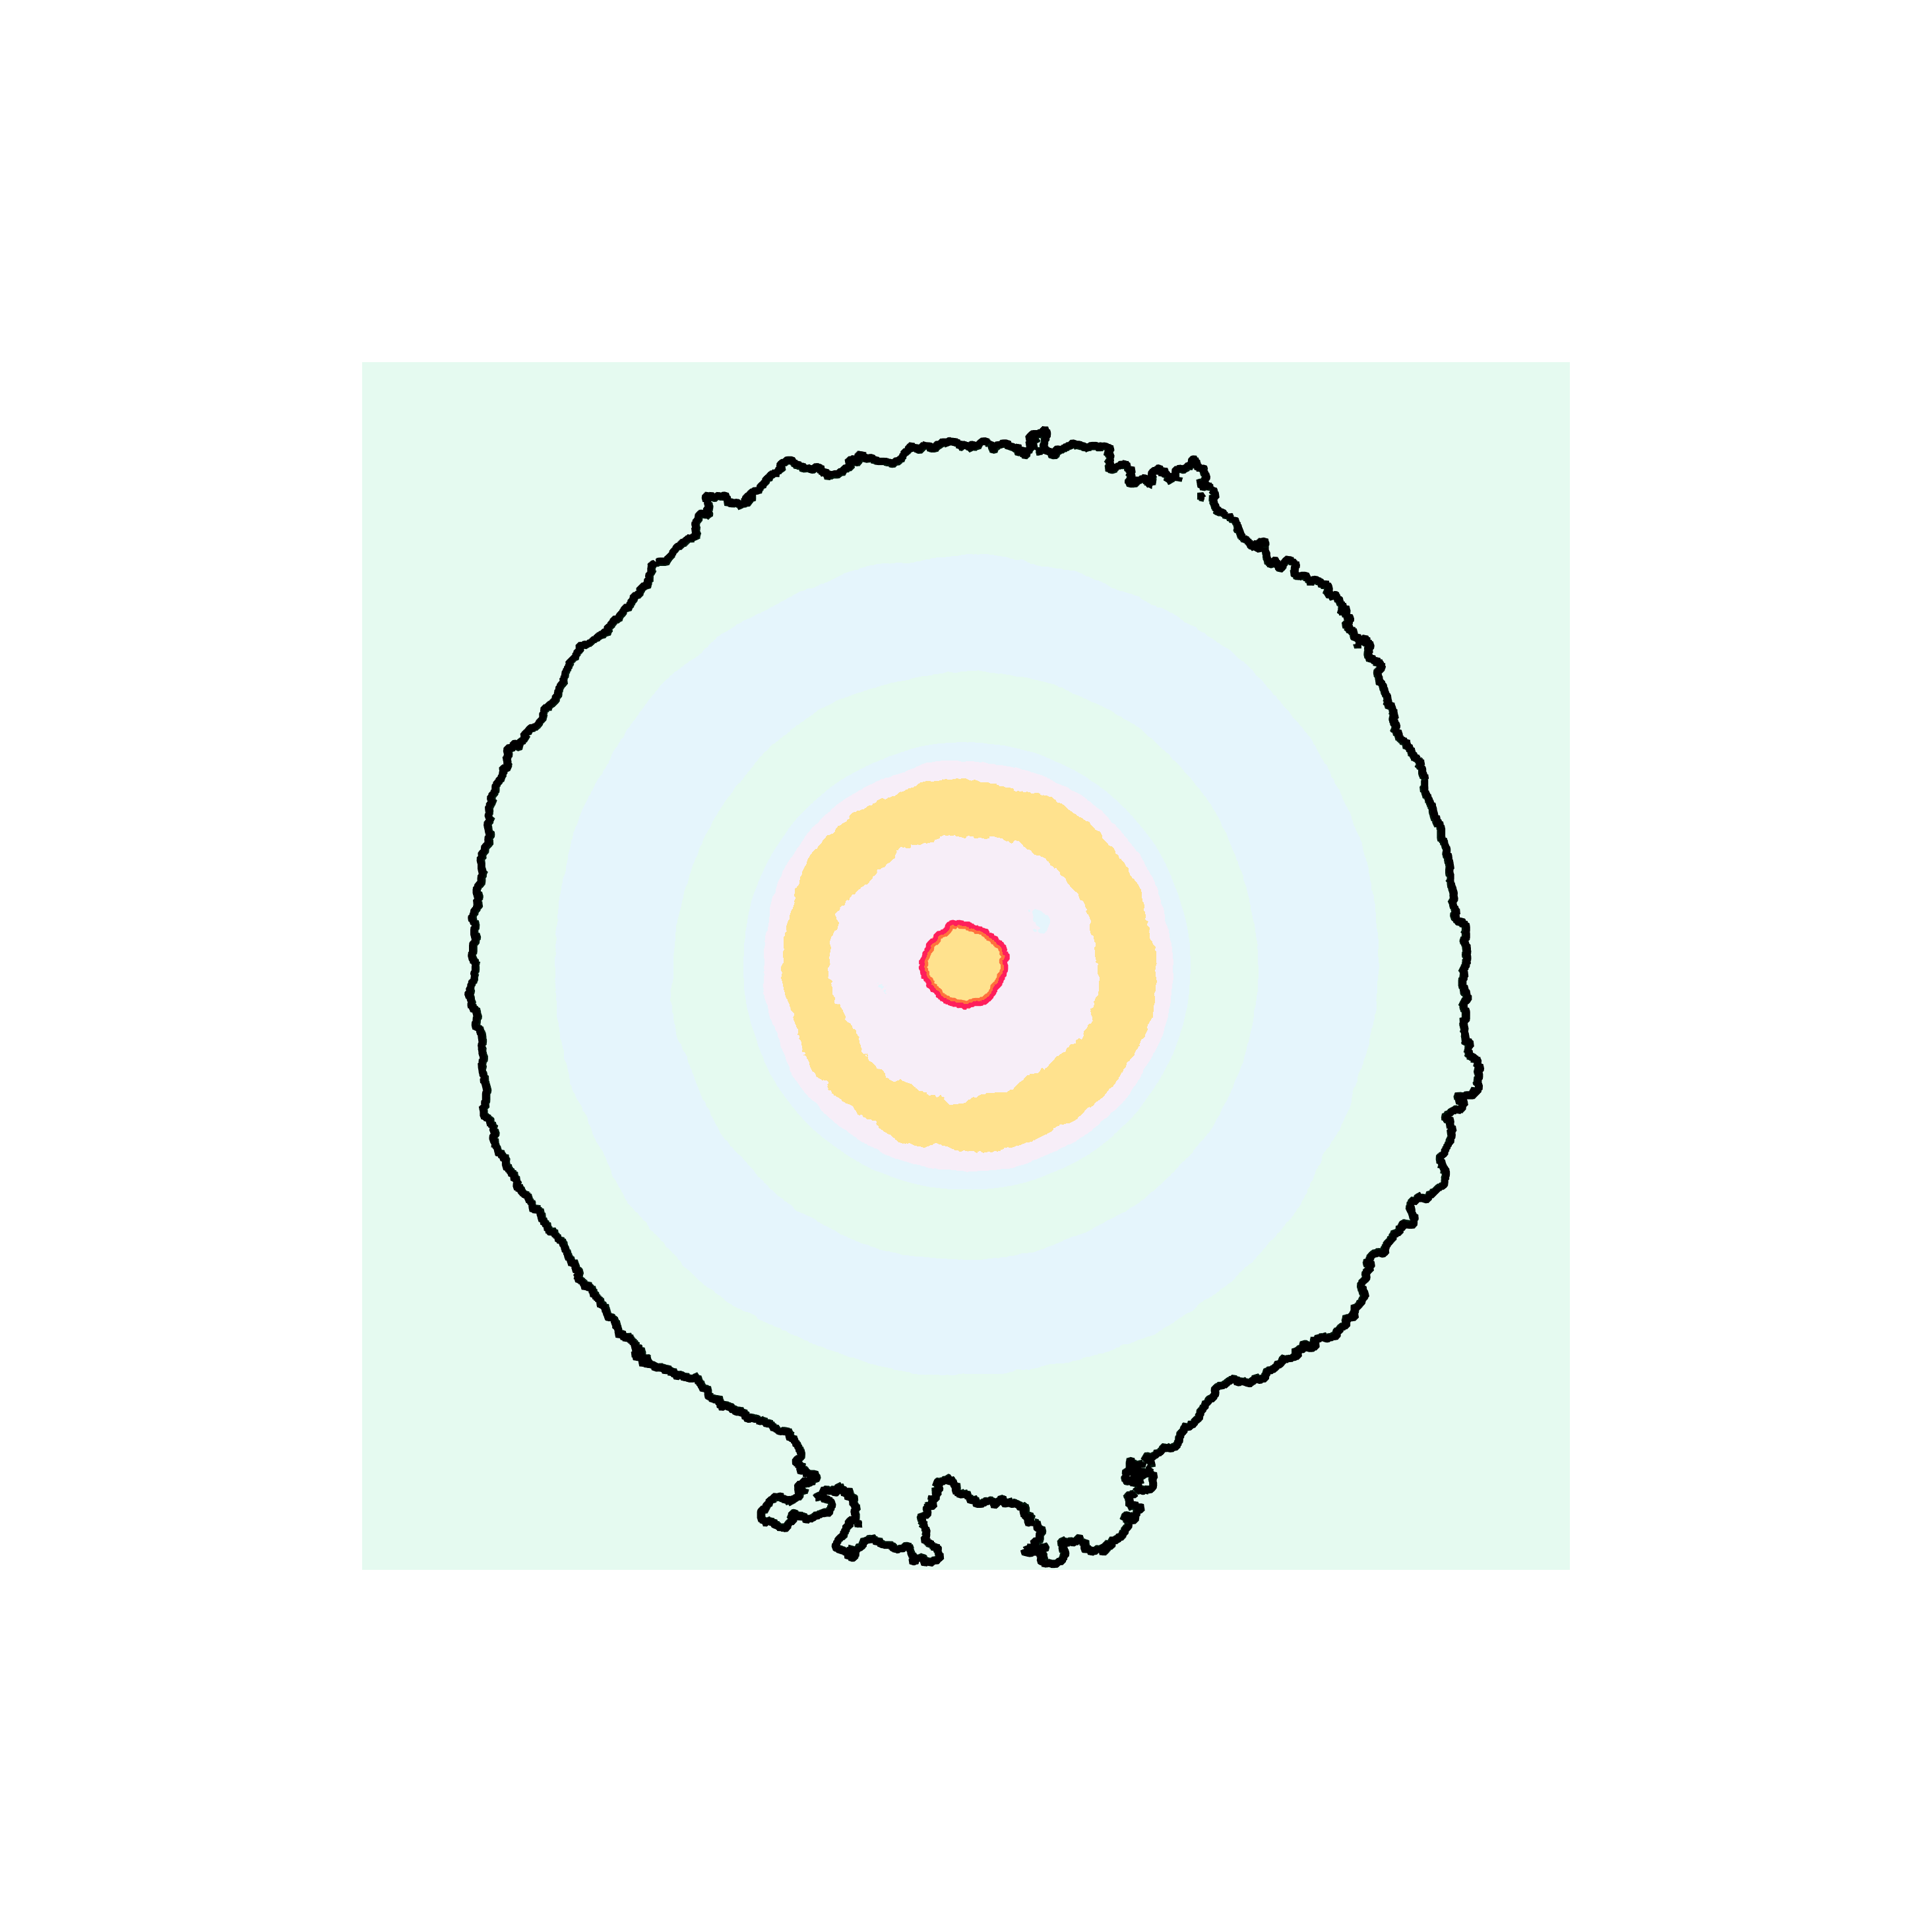
\includegraphics[trim=500 500 500 500, clip, width=0.24\textwidth]{figures/matching-surf_top-1_2.png}
  \caption{(Top) $\hom_1$ persistence diagrams of the function depicted in Figure~\ref{fig:ripple1} restricted to \emph{superlevel} sets at $\omega = 0.3, 0.5,$ and $0.7$ (on a $1024\times 1024$ grid).
  The matching is shown between a feature in the full diagram (marked with a diamond) with its representative cycle in black.
  The corresponding representative cycle in the restricted diagram is pictured in red.}\label{fig:restricted}
\end{figure}

Figure~\ref{fig:restricted} shows this distance for a feature that persists throughout the diagram.
As the restricted diagram in full resolution the restricted filtration is a subset of the full filtration, so these features can be matched by their death simplices.
For illustrative purposes we also show the representative cycles associated with these features.

We imagine a setting where we would like to classify a function using a sample that cannot be verified below some known $\omega$.
That is, we can only check for coverage of the superlevel set $D\setminus B_\omega$ using the variation of the TCC we have introduced in the previous sections.
We would then like to classify the function with the bottleneck distance to a set of known functions based on the region we cover.
However, as we have shown, the restricted diagram may contain artifacts of features born before $\omega$ which will skew our measurement.
Instead, as $\omega$ is known, we can compare the \emph{relative} diagram the collection of \emph{truncated} diagrams of known functions to get a better classification.

\paragraph*{Relative diagrams and reconstruction.}

\begin{figure}[htbp]
  \centering
  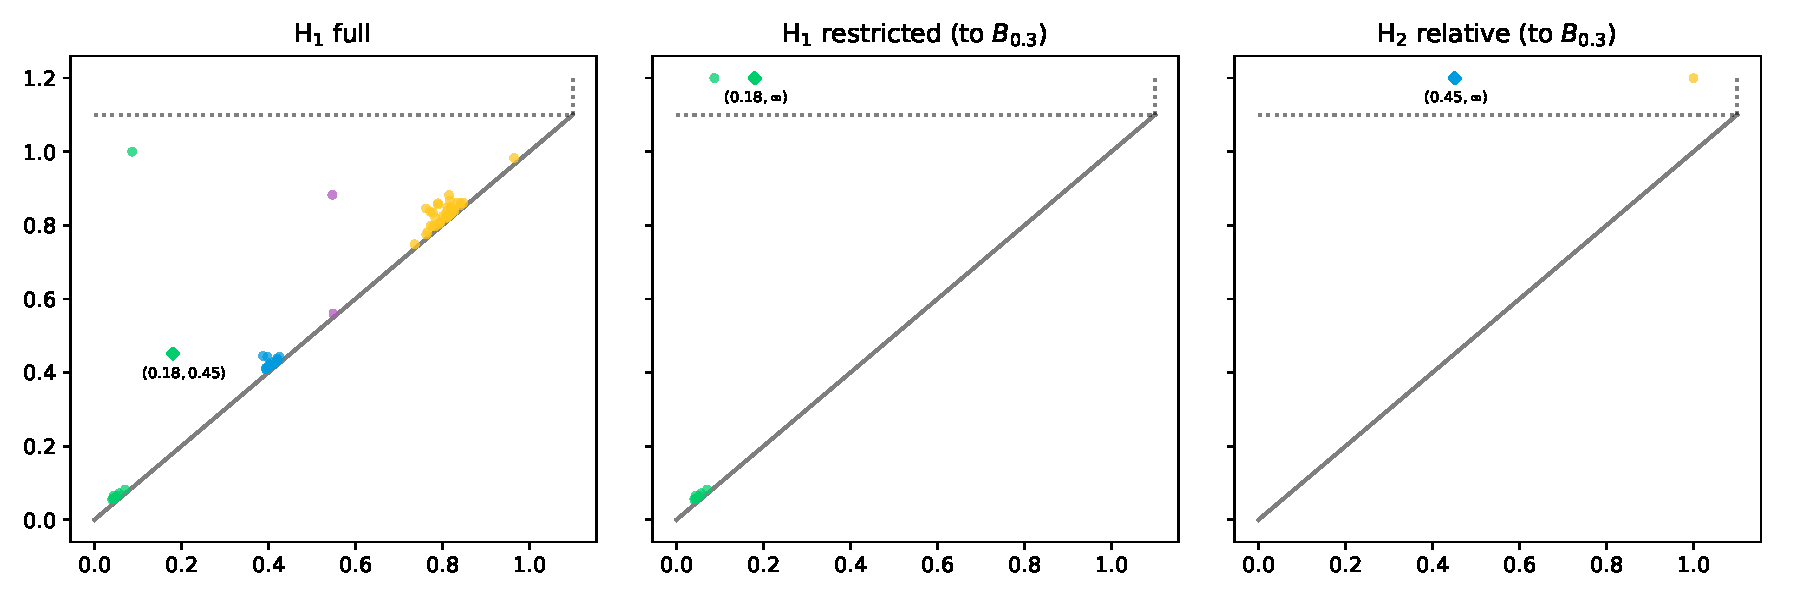
\includegraphics[width=0.9\textwidth]{figures/relative-dgm-0_0.pdf}
  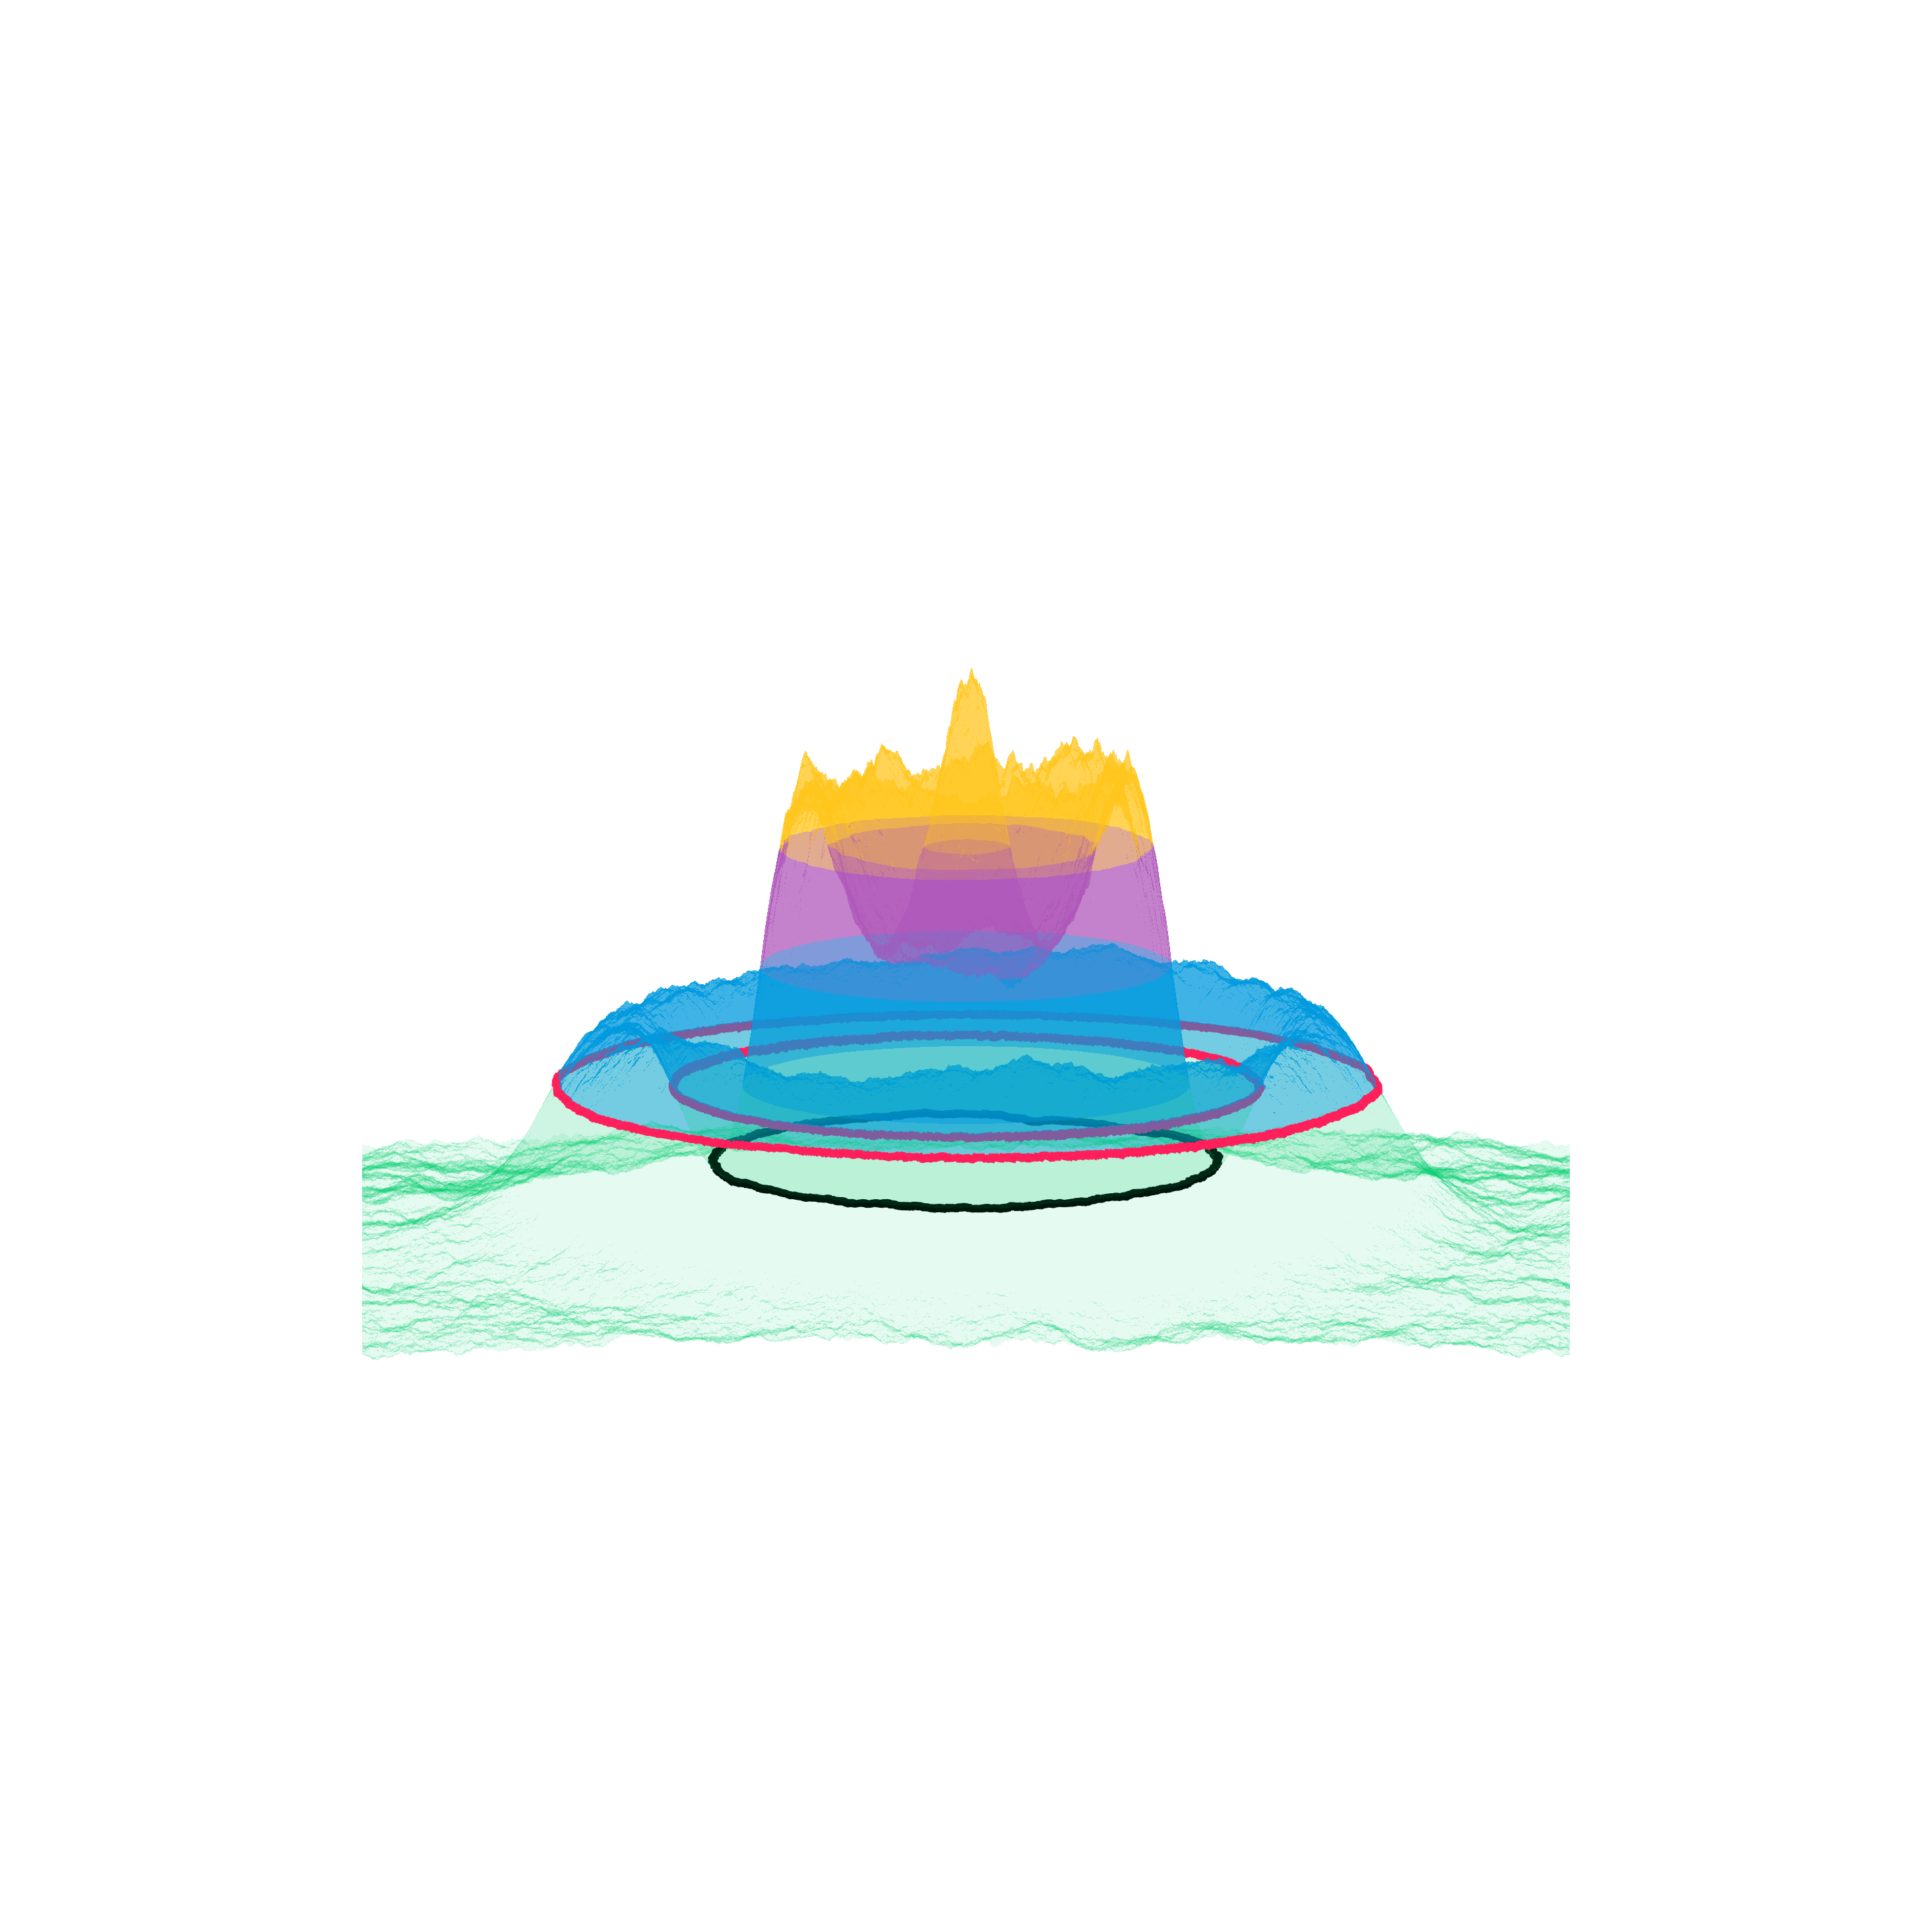
\includegraphics[trim=500 800 500 800, clip, width=0.35\textwidth]{figures/relative-surf_side-0_0.png}
  
\includegraphics[trim=500 500 500 500, clip, width=0.25\textwidth]{figures/relative-surf_top-0_0.png}
  % \caption{(Left) Full $\hom_1$ persistence diagram, (middle) $\hom_1$ persistence diagram of the function restricted to the \emph{sub}-levelset $B_{0.3}$, (right) $\hom_2$ persistence diagram of the the function realtive to the sub-levelset $B_{0.3}$.
  \caption{(Top) The indicated infinite features in the restricted and relative diagrams correspond to the birth and death of the 1-feature $(0.18, 0.45)$ in the full diagram.
  (Bottom) In black, the representative cycle of the infinite 1-feature born at 0.18 in the restricted diagram is shown in black.
  In red, the \emph{boundary} of the representative \emph{relative} 2-cycle born at 0.45 in the relative diagram is shown in red.}\label{fig:relative1}
\end{figure}

Now, imagine we obtain the persistence diagram of our sublevel set $B_\omega$.
That is, we now know that we cover $B_\omega$, or some subset, and do not want to re-compute the diagram above $\omega$.
If we compute the persistence diagram of the function restricted to the \emph{sublevel} set $B_\omega$ any 1-dimensional features born before $\omega$ that die after $\omega$ will remain infinite features in this restricted (below) diagram.
Indeed, we could match these infinite 1-features with the corresponding shifted finite 1-features in the restricted (above) diagram, as shown in Figure~\ref{fig:restricted}.
However, that would require sorting through all finite features that are born near $\omega$ and deciding if they are in fact features of the full diagram that have been shifted.

Recalling that these same features become infinite 2-features in the relative diagram, we can use the relative diagram instead and match infinite 1-features of the diagram restricted below to infinite 2-features in the relative diagram, as shown in Figures~\ref{fig:relative1} and~\ref{fig:relative2}.
For this example the sequence of birth times of relative 2-features in \emph{decreasing} order correspond to the deaths of restricted 1-features in \emph{increasing} order.
How to construct this matching in general, especially in the presence of infinite features in the full diagram, is the subject of future research.

\begin{figure}[htbp]
  \centering
  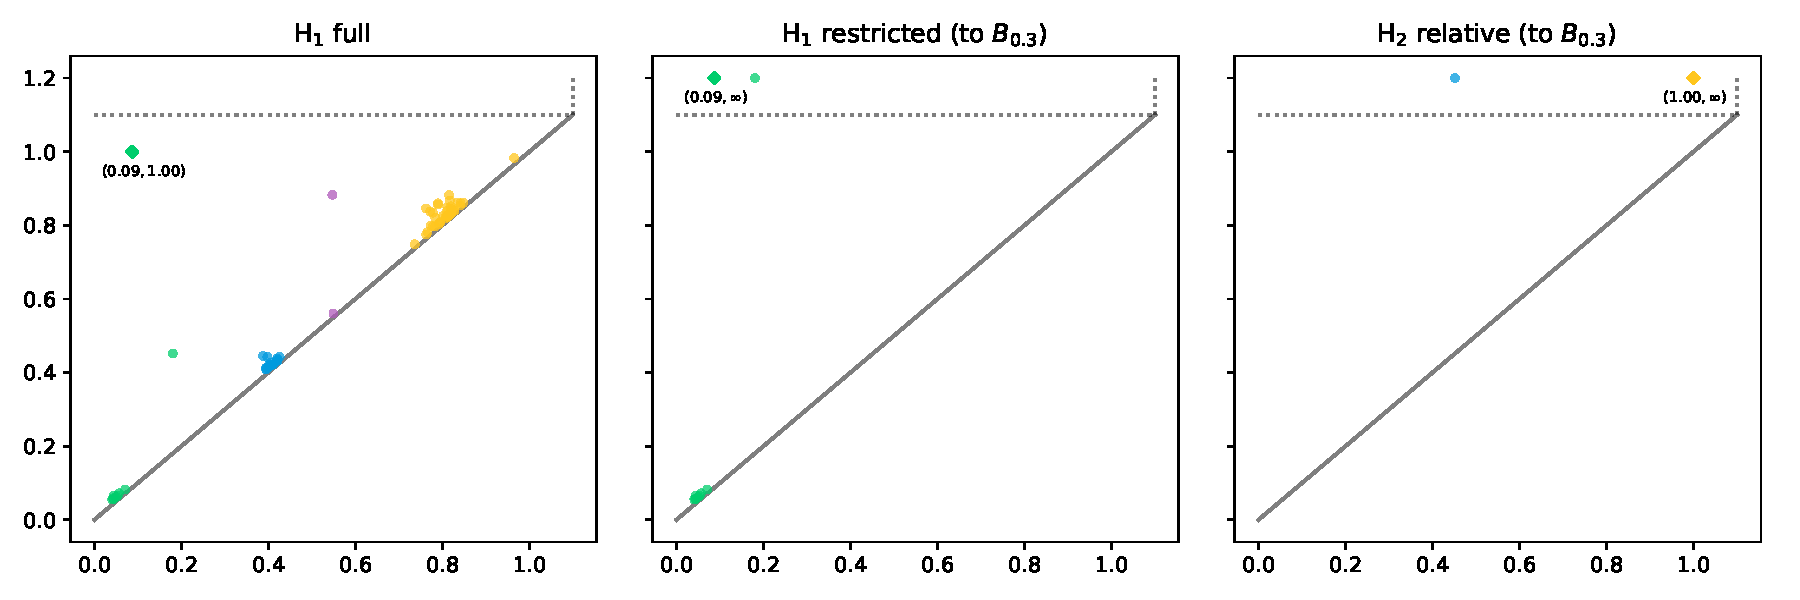
\includegraphics[width=0.9\textwidth]{figures/relative-dgm-0_1.pdf}
  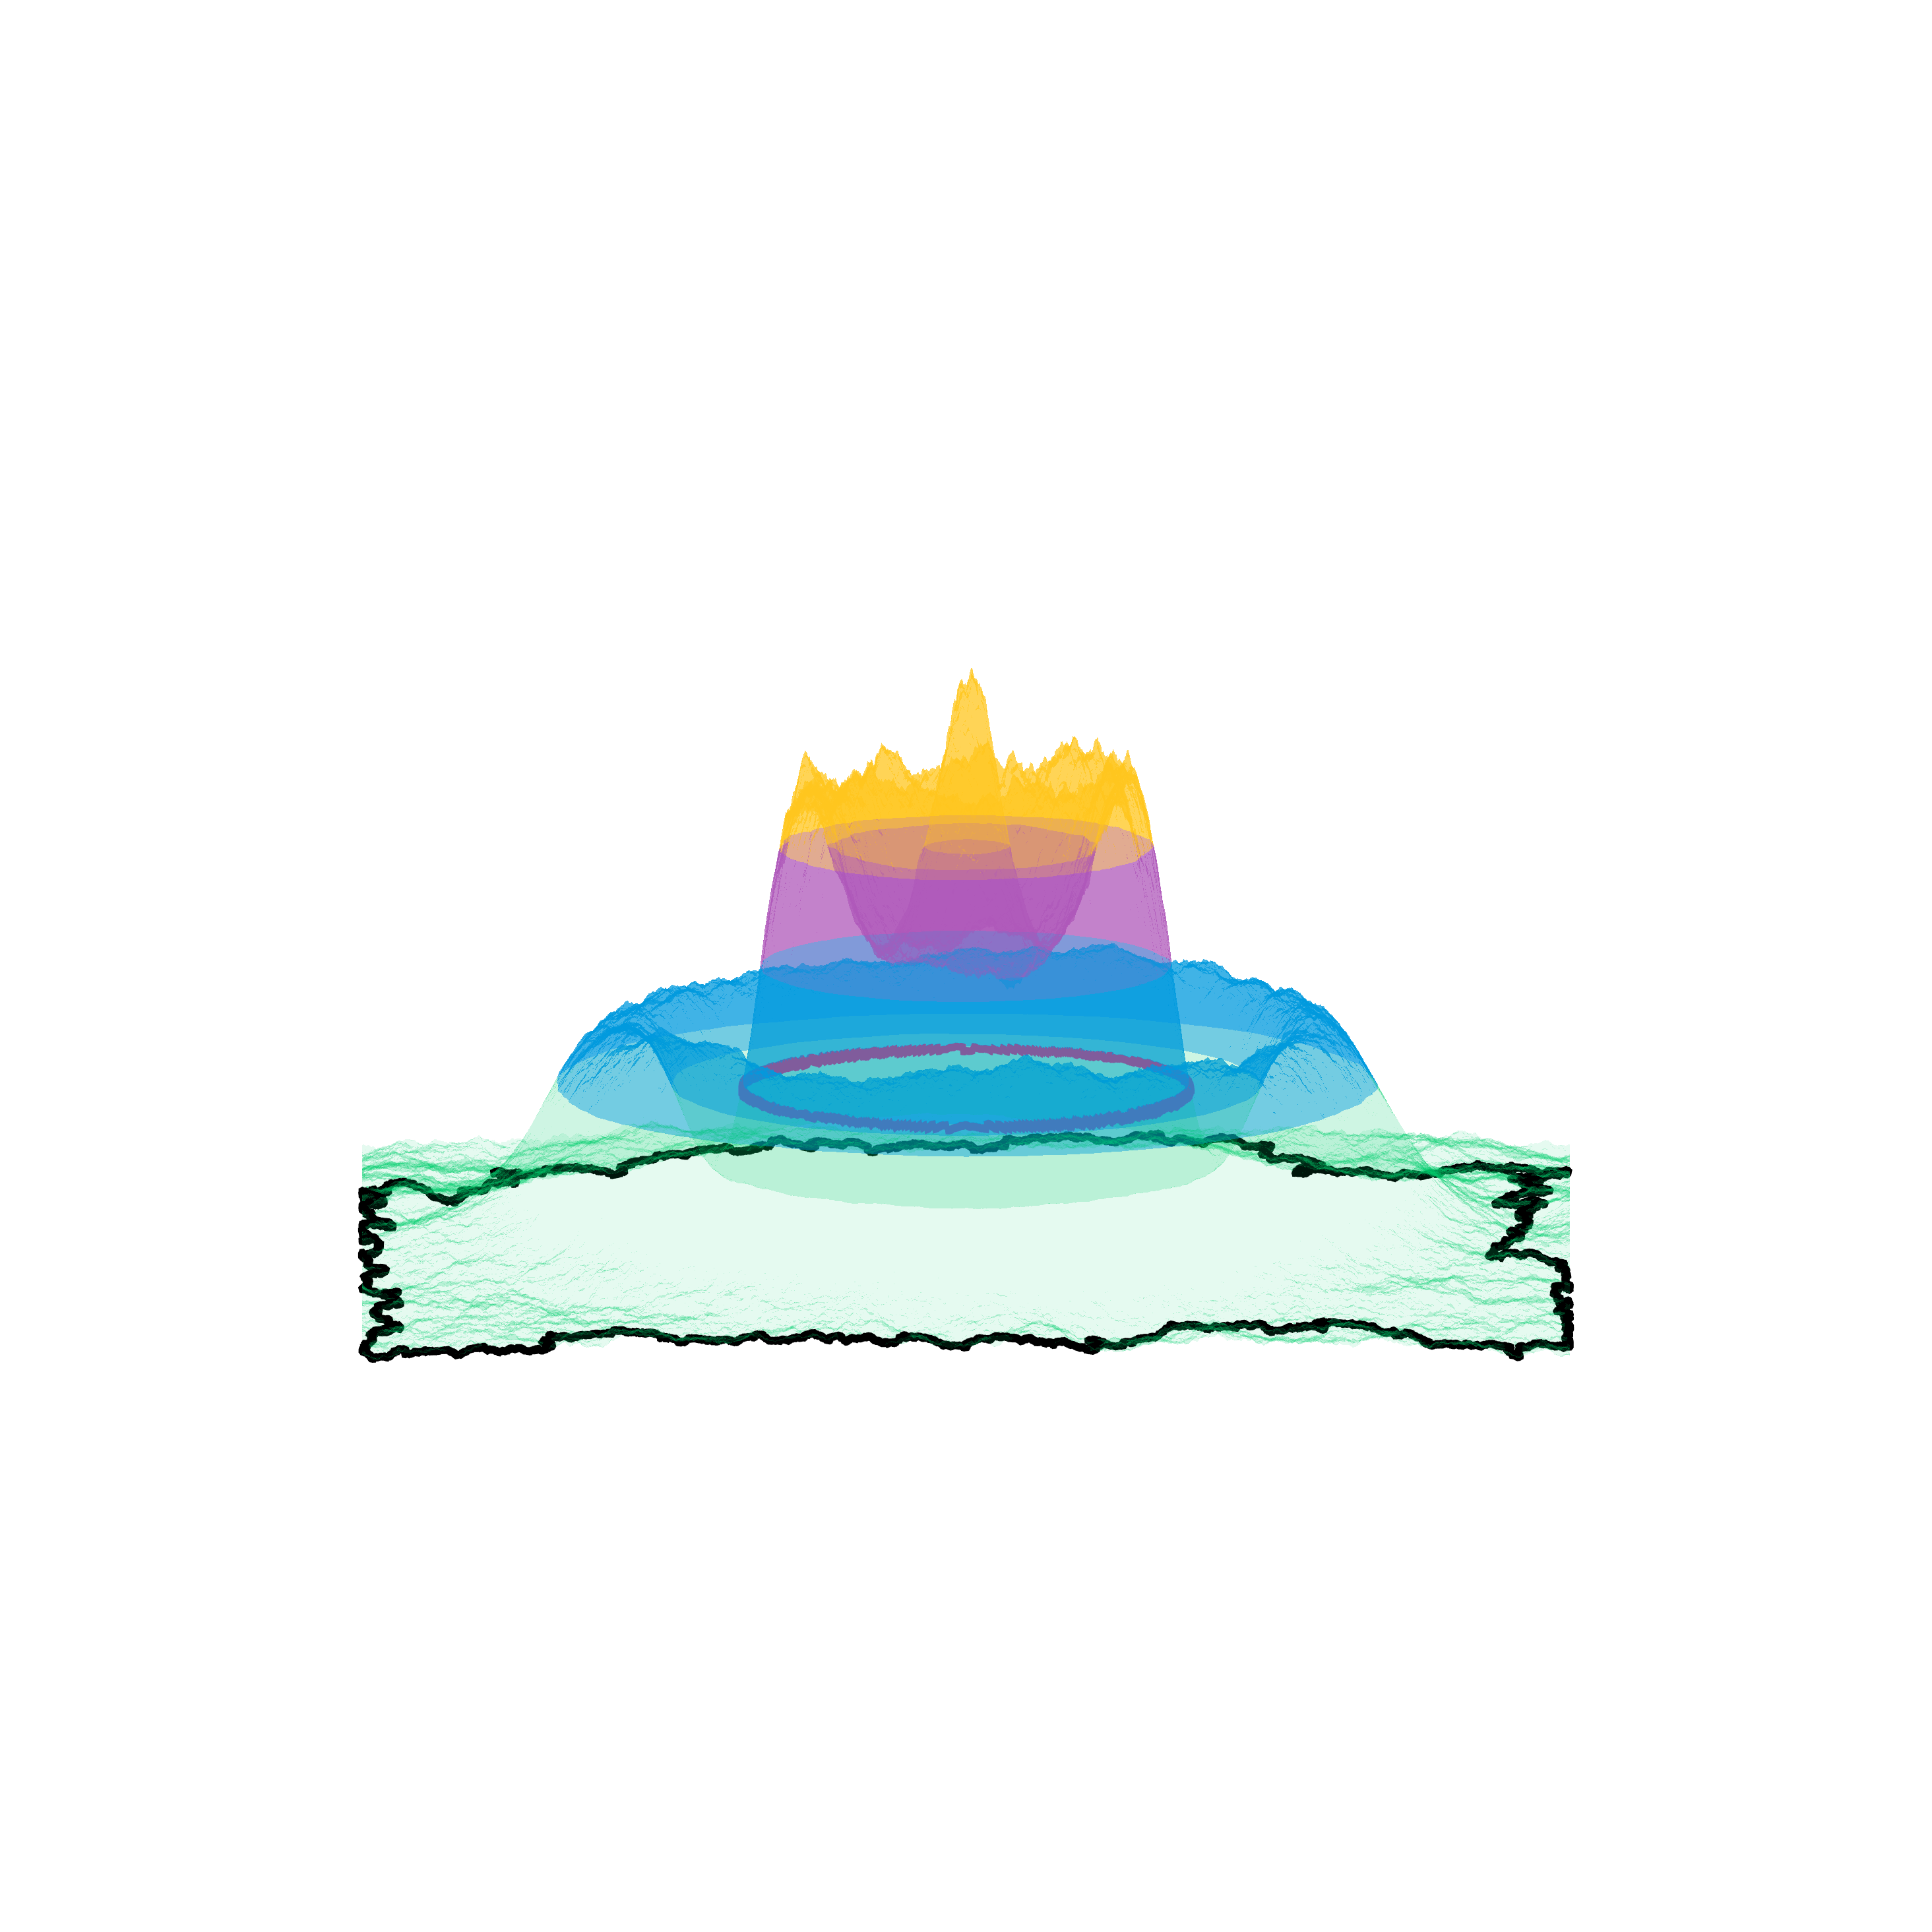
\includegraphics[trim=500 800 500 800, clip, width=0.35\textwidth]{figures/relative-surf_side-0_1.png}
  
\includegraphics[trim=500 500 500 500, clip, width=0.25\textwidth]{figures/relative-surf_top-0_1.png}
  \caption{The infinite 1-features of the restricted diagram can be matched with the infinite 2-features of the relative diagrams.
  The sequence of birth times of relative 2-features in \emph{decreasing} order correspond to the deaths of restricted 1-features in \emph{increasing} order.}\label{fig:relative2}
\end{figure}

  % \clearpage
  %
  % \section{Conclusions}
  % \input{trajectories}
  % \input{future}

  \bibliographystyle{unsrt}
  \bibliography{bibliography}
\end{document}
